\documentclass[11pt,reqno]{amsart}
\usepackage[T1]{fontenc}
\usepackage[utf8]{inputenc}
\usepackage{lmodern}
\usepackage{amsmath,amssymb,amsthm,mathrsfs}
\usepackage{geometry}
\geometry{a4paper,margin=30mm}
\usepackage{microtype}
\usepackage{graphicx,booktabs,array}
\usepackage{enumitem}
\setlist{itemsep=3pt,topsep=5pt}
\usepackage{xcolor}
\definecolor{linkblue}{RGB}{31,70,105}
\usepackage{tikz}
\usetikzlibrary{arrows.meta,positioning,calc,decorations.pathmorphing,fit}
\usepackage[colorlinks=true,linkcolor=linkblue,citecolor=linkblue,urlcolor=linkblue,
  pdfauthor={OpenAI},pdftitle={A boundary-only obstruction to four-dimensional disk embedding}]{hyperref}
\numberwithin{equation}{section}
\newtheorem{theorem}{Theorem}[section]
\newtheorem{proposition}[theorem]{Proposition}
\newtheorem{lemma}[theorem]{Lemma}
\newtheorem{corollary}[theorem]{Corollary}
\theoremstyle{definition}
\newtheorem{definition}[theorem]{Definition}
\theoremstyle{remark}
\newtheorem{remark}[theorem]{Remark}
\newtheorem{convention}[theorem]{Convention}
\newcommand{\C}{\mathbb C}
\newcommand{\Z}{\mathbb Z}
\newcommand{\R}{\mathbb R}
\newcommand{\Q}{\mathbb Q}
\newcommand{\F}{\mathbb F}
\DeclareMathOperator{\tr}{tr}
\DeclareMathOperator{\Ad}{Ad}
\DeclareMathOperator{\End}{End}
\DeclareMathOperator{\Hom}{Hom}
\DeclareMathOperator{\im}{im}
\DeclareMathOperator{\rank}{rank}
\DeclareMathOperator{\SL}{SL}
\DeclareMathOperator{\Spec}{Spec}
\DeclareMathOperator{\Res}{Res}
\DeclareMathOperator{\id}{id}
\title[A boundary-only obstruction to disk embedding]{A boundary-only obstruction to four-dimensional disk embedding}
\author{\NoCaseChange{OpenAI}}
\date{September 24, 2026}
\begin{document}
\begin{abstract}
We disprove the four-dimensional disc embedding conjecture without a
fundamental-group hypothesis, even when no homotopy classes or output framings
are prescribed. We construct a compact oriented smooth four-manifold containing
finitely many disc maps with framed algebraic dual spheres whose boundary
circles bound no disjoint locally flat discs. Consequently, the free group on
two generators is not good in the sense of Freedman--Quinn, and neither is any
group containing it as a subgroup.
\end{abstract}
\maketitle
\clearpage
\tableofcontents
\clearpage
\section{Introduction}\label{sec:introduction}

The Whitney trick is the geometric step that turns algebraic cancellation
of intersections into disjoint embedded surfaces. In dimension four,
the Whitney discs needed for this step may themselves meet the surfaces
one is trying to separate. The disc embedding problem asks whether
algebraic intersection data, supplemented by suitable dual spheres,
suffice to produce the embedded discs. Its solution for good fundamental
groups underlies topological surgery and the five-dimensional
$s$-cobordism theorem for four-manifolds
\cite[Theorem~5.1A and Chapters~7 and~11]{FQ1990}.

Here is the formulation we use. Let $M$ be an oriented four-manifold,
let $\pi=\pi_1(M)$, and fix basing paths, or \emph{whiskers}, for all
surfaces. The equivariant intersection pairing $\lambda$ records an
intersection point with its sign and the element of $\pi$ obtained from
these paths; its values lie in $\Z[\pi]$. A family of sphere maps
$g_j$ is algebraically dual to disc maps $f_i$ if
$\lambda(f_i,g_j)=\delta_{ij}1$. A geometric dual meets its corresponding
disc in one transverse point and misses the other discs. We use the
reduced Wall invariant
\begin{equation}\label{eq:wall-convention}
 \widetilde\mu\colon\pi_2(M)\longrightarrow
 \Z[\pi]/\langle h-h^{-1},\,\Z\cdot1\rangle_{\mathrm{add}}.
\end{equation}
The quotient is additive, rather than a quotient by a group-ring ideal;
these are the oriented conventions of \cite[Section~1.3]{PRT2025}.

The disc embedding theorem applies to disc maps with disjoint locally
flatly embedded boundaries and algebraic dual spheres satisfying
$\lambda(g_i,g_j)=0=\widetilde\mu(g_i)$. When $\pi$ is good, it produces
disjoint locally flat discs with those boundaries, with geometric duals,
and with the induced boundary framings preserved for generically
immersed input discs \cite[Theorem~A]{PRT2025}.
The unrestricted disc embedding conjecture asks for this implication
without the good-group assumption. Theorem~\ref{thm:main} disproves it
by excluding every disjoint locally flat filling of the specified
boundary circles, even when no output framing or dual sphere is required.

\begin{theorem}\label{thm:main}
There exist a compact connected oriented smooth four-manifold $M$ with nonempty boundary, an integer $k\geq1$, proper generically immersed discs
\[
 f_i\colon(D^2,S^1)\longrightarrow(M,\partial M),\qquad 1\leq i\leq k,
\]
whose boundary restrictions form an embedding of $\coprod_iS^1$, and framed sphere maps $g_i\colon S^2\to M$ such that
\begin{equation}\label{eq:input-invariants}
 \lambda(f_i,g_j)=\delta_{ij}\,1,\qquad
 \lambda(g_i,g_j)=0,\qquad
 \widetilde\mu(g_i)=0
 \quad(1\leq i,j\leq k),
\end{equation}
but the given boundary circles do not bound pairwise disjoint proper locally flat embedded discs in $M$. Each $g_i$ can be chosen to be a smooth embedded sphere; different $g_i$ are allowed to intersect.
\end{theorem}

The boundary condition in this formulation is classical. The additional
force of the conclusion is its nonexistence assertion: changing the
relative homotopy classes of the prospective discs cannot evade the
obstruction. The vanishing assumptions are placed on the dual spheres;
no vanishing of the intersections among the input discs is needed.

\subsection{Good groups and the free-group problem}

Casson supplied the handle-embedding construction that makes the
simply connected theory possible. Freedman proved that every Casson
handle is homeomorphic, relative to its attaching region, to an open
two-handle \cite[Theorems~3.1 and~1.1]{Freedman1982}. Together these
results replace the unavailable smooth Whitney discs by topological
ones. Freedman--Quinn developed a version using capped gropes, obtained
by attaching surfaces along symplectic basis curves and closing the
upper curves with immersed caps \cite[Chapters~2--5]{FQ1990}.
The caps may intersect; the loops through these intersections carry
the fundamental-group information that must be controlled.

Goodness is a local condition on such models. In the formulation of
\cite[Definition~3.2]{PRT2025}, every height-$1.5$ disc-like capped
grope, equipped with a homomorphism from its fundamental group to the
group in question, must have an immersed disc in its four-dimensional
thickening with the same framed boundary whose double-point loops map
to the identity. A height-$1.5$ grope has a first surface stage with
further surface stages attached along one curve from each symplectic
pair; its remaining tips are capped.
The thickenings used in this test have free fundamental groups, which
explains the central role of the free-group case
\cite[pp.~510--511]{FT1995}.

Freedman--Teichner extended the positive theory to all groups of
subexponential growth \cite[Theorem~0.1]{FT1995}. Krushkal--Quinn gave
a different proof based on splitting gropes into dyadic branches and
organizing the resulting double-point words \cite[p.~408]{KQ2000}.
Their paper also contains the correction to the earlier height-raising
argument. The known class is closed under subgroups, quotients,
extensions and directed colimits; it includes finite and solvable groups as
well as groups of subexponential growth
\cite[Section~1.1]{PRT2025}. Thus exponential growth alone does not
mark the boundary of the theorem. The nonabelian free-group case
remained open in the 2025 account \cite{PRT2025}; see also
\cite[Chapter~23]{KOPR2021} for its place among four-manifold problems.

The construction of geometric dual spheres requires attention even
in the positive theory. Powell--Ray--Teichner supplied the missing
construction in the proof of Freedman--Quinn's theorem and also
controlled the homotopy classes of those duals
\cite[Theorem~A and Remark~1.3]{PRT2025}. Their correction concerns
output geometric duals and is distinct from the height-raising
correction in \cite{KQ2000}.

\begin{corollary}[Nongoodness of the free group]\label{cor:nongood}
The free group $F_2$ on two generators is not good in the sense of
Freedman--Quinn. Every group containing a subgroup isomorphic to $F_2$
is likewise not good.
\end{corollary}
\begin{proof}
The group $\pi_1(M)$ of the manifold in Theorem~\ref{thm:main} is
finitely presented because compact smooth manifolds have finite CW
homotopy type. It is not good: otherwise \cite[Theorem~A]{PRT2025},
applied to the discs and spheres in \eqref{eq:input-invariants}, would
supply the forbidden embedded discs.

Choose a finite generating list for $\pi_1(M)$ of length $r\geq2$,
padding if necessary. There is then a surjection
$F_r\twoheadrightarrow\pi_1(M)$. The elements $a^jba^{-j}$ for
$0\leq j<r$ freely generate a rank-$r$ subgroup of
$F_2=\langle a,b\rangle$, as follows from reduced-word normal form.
Subgroups and quotients of good groups are good
\cite[Section~1.1, p.~4]{PRT2025}. If $F_2$ were good, its subgroup
$F_r$ and then the quotient $\pi_1(M)$ would be good, a contradiction.
Finally, a good group containing a subgroup isomorphic to $F_2$ would
make $F_2$ good by subgroup closure, which proves the last assertion.
\end{proof}

The conclusion about $F_2$ is group-theoretic: it does not identify
$\pi_1(M)$ with $F_2$, and the geometric counterexample remains the
one in Theorem~\ref{thm:main}.

\subsection{Surgery and previous obstruction approaches}

The free-group problem also has concrete link formulations. Freedman
asked whether the Borromean rings are $A$--$B$ slice
\cite{Freedman1986AB}. Here each component is assigned a decomposition
$D^4=A_i\cup B_i$ extending the standard genus-one decomposition of
$S^3$. One seeks disjoint copies of all the pieces with attaching
curves given by the link and a parallel copy; each copy must extend
to an ambient self-homeomorphism of $D^4$. Freedman--Lin relate this
condition for the full generalized Borromean family to topological
surgery, equivalently to slicing the corresponding Whitehead doubles
with meridians freely generating the slice-complement group
\cite[pp.~91--92]{FL1989}.

Two results show why this obstruction program is delicate. Krushkal
proved that every link with vanishing pairwise linking numbers is
weakly $A$--$B$ slice, where the ambient-extension requirement is
removed \cite[Theorem~1 and Definition~2.4]{Krushkal2008}.
Freedman--Krushkal subsequently constructed homotopy $A$--$B$ slices
for the universal generalized Borromean family using the $2$-Engel
relation \cite[Theorem~1 and Definition~3.10]{FK2016}.
These are positive results for weakened embedding problems. The
present obstruction instead starts from the actual images of
hypothetical embedded discs and extracts restrictions on them through
representation deformations. The independent conjugates of all triple
commutators used here are specified in Section~\ref{sec:geometry};
they are not an invocation of the Engel relation.

Positive surgery results for free fundamental groups also persist in
important special cases. Krushkal--Lee solve the unobstructed surgery
problem for a degree-one normal map from a closed four-manifold to a
Poincare complex with free fundamental group, when the target
intersection pairing is extended from the integers
\cite[Theorem~1]{KL2002}. Their proof cuts along inverse images of
points under a map to a graph and reduces the stabilized problem to
the simply connected case. In our construction the corresponding
cuts have torus boundaries. Their boundary restriction data are
retained throughout the obstruction; the closed-manifold result does
not supply fillings for them \cite[Introduction, Remark]{KL2002}.

For precision, we use the following two unrestricted assertions in
the sense of \cite[Conjectures~1.5--1.6]{KPT2021}. The
\emph{topological surgery assertion} says that a degree-one normal
map from a compact four-manifold to a four-dimensional Poincare pair
$(Z,\partial Z)$, which is a $\Z[\pi_1(Z)]$-homology equivalence on the boundary and has
zero Wall surgery obstruction, is normally bordant relative to the
boundary to a homotopy equivalence. The \emph{$s$-cobordism assertion}
says that every compact five-dimensional topological $s$-cobordism
with a specified product on its boundary is homeomorphic to a product
extending that boundary structure. Neither assertion restricts the
fundamental group.

\begin{corollary}\label{cor:surgery-conjunction}
The unrestricted topological surgery and $s$-cobordism assertions
cannot both hold.
\end{corollary}
\begin{proof}
Together these assertions imply the unrestricted disc embedding
conjecture \cite[Section~3]{KPT2021}. Its algebraic hypotheses apply
to the finite family of discs and framed spheres in the compact
manifold of Theorem~\ref{thm:main}, so it
would give the excluded boundary filling.
\end{proof}

The corollary concerns their conjunction; it does not determine which
assertion fails. In particular, the free-group conclusion above is
not being used as a substitute for the quoted equivalence.

\subsection{The obstruction}
The construction starts with a smooth four-manifold having the homotopy type of a finite graph. A finite family of capped gropes inside it encodes every triple commutator of suitably conjugated end generators. Removing neighborhoods of the grope bases gives the actual manifold $M$. The shallow caps are the input discs. Product tori, compressed using the upper stages, give the spheres in \eqref{eq:input-invariants}. The proof checks their framings and all equivariant cancellation labels in $\pi_1(M)$.

Suppose disjoint locally flat discs with the prescribed boundaries existed. They would permit a graph map to be altered near their images and then cut along regular levels. The resulting three-dimensional walls have one torus boundary apiece, and the complementary four-dimensional region carries the triple commutator relations. An adjoint $\SL_2(\C)$ local system turns these relations into a cube-zero ideal in a representation deformation ring. A two-sheeted Mayer--Vietoris calculation supplies two complementary tangent spaces.

The comparison of representation deformations and flat connections has
a classical differential graded Lie algebra formulation in
Goldman--Millson \cite[Proposition~2.6 and Section~6]{GM1988}.
Here finite transition-cochain charts retain the equations themselves,
which will be needed with their full ideal structure.

To describe the resulting obstruction, label the walls $1,\ldots,d$.
Write $a_i\in\C^3$ for holonomy coordinates centered at the identity
along a chosen boundary circle on the $i$th wall's torus, and $y_i$ for its remaining deformation
coordinates. Its function $P_i(a_i,y_i)$ is a boundary-polarized version
of the Chern--Simons transgression integral
\cite[Section~3]{ChernSimons1974}.
Write $a=(a_i)_i$, and let $t$ be the remaining deformation parameters
of the cut four-manifold. Label its two copies of each wall so that
the chosen holonomy may vary on the positive copy and is trivial on
the negative copy. Their restrictions then have the form
$(a_i,Y_i^+(a,t))$ and $(0,Y_i^-(a,t))$.
Let $Y=(Y_i^+,Y_i^-)_i$, and let $C=(C_i^+,C_i^-)_i$ be independent
tuples with each $C_i^\pm$ of the same size as $y_i$. Put
\[
 \Psi(a,C)=\sum_i\bigl(P_i(a_i,C_i^+)-P_i(0,C_i^-)\bigr),
 \qquad
 v(a,t)=(\partial_C\Psi)(a,Y(a,t)).
\]
Here differentiation precedes restriction to the graph $C=Y(a,t)$.
If $\mathfrak r$ is the ideal of equations for the four-dimensional
representation chart, the two identities are
\[
                  (v)=\mathfrak r,
           \qquad \Psi(a,Y(a,t))\in\mathfrak r^2.
\]
The first identifies the whole ideal, including its nilpotent
information. If the derivatives missed an equation, the resulting first
obstruction to flatness would pair trivially with every wall variation.
Duality and the paired Mayer--Vietoris isomorphism would then kill its
curvature class, permitting a flat lift that contradicts the minimality
of the defect equations. The second identity comes from comparing the wall
connections on the closed boundary of the cut manifold: Stokes turns
their total value into an integral of curvature squared.

Choose one scalar coordinate $a_{i,1}$ on each wall and set
$p_i(y_i)=\partial_{a_{i,1}}P_i(0,y_i)$. The end-holonomy cube law
gives two distinct families of memberships, for every triple of labels:
\[
 a_{i,1}a_{j,1}a_{k,1}\in(v),\qquad
 p_i(Y_i^-)p_j(Y_j^-)p_k(Y_k^-)\in(v).
\]
The boundary term in polarized variation places each $p_i(Y_i^-)$
in the end-deviation ideal modulo $\mathfrak r$, giving the second family.
These are ideal memberships with coefficients, stronger than statements
about the common zero set.

The next step makes these identities available in positive
characteristic. All gradient jets of each original $P_i$ have
representatives in one fixed smooth complex algebraic chart. This
allows replacement of $P_i$, to sufficiently high order along its wall
ideal, by an algebraic germ. The replacement uses exactness and faithful
flatness of completion \cite[Tags 00MA--00MC]{Stacks} and differential
tests for symbolic powers \cite[Theorem~3.6 and Lemma~2.3]{DSGJ2020}.
The square-value identity then permits a
formal correction of $Y$ making $\Psi$ vanish exactly on the corrected
graph. An invertible change of gradient generators transports both
displayed cubic memberships to that graph. Only finitely many constants
and inverse Jacobians are needed for the new potentials, the correction
and its membership witnesses, so all these data specialize to a field
$\Bbbk$ of positive characteristic. The corrected graph need not describe
representations; the original end-holonomy cube law has already supplied
the two memberships that the remaining argument uses.

In characteristic $\ell$, quotienting by the separate $\ell$th powers
of the coordinates gives a finite-dimensional complex of differential
forms. The corrected graph at $a=0$ and its copy with the positive and
negative blocks exchanged have complementary tangent spaces, and the
potential vanishes on both. They determine cohomology classes with
nonzero pairing. Using this pairing and the cubic law for the $p_i$,
we construct, when there are at least five walls, two classes in a
deformation of the complex whose pairing is a unit in the deformation
ring. The cubic law for the $a_{i,1}$ then forces a nonzero parameter
product times that pairing to vanish. Section~\ref{sec:frobenius}
constructs this contradiction in the finite complex.

Lemma~\ref{alg:replacement} and Theorem~\ref{frob:no-data} are stated independently of the geometric construction. They are available for other problems meeting their respective stated hypotheses; in Theorem~\ref{frob:no-data} these include both cubic ideal-membership laws. No additional application is asserted here.

\subsection{Conventions and organization}
All manifolds used in the construction are compact and smooth until the hypothetical locally flat discs are introduced. Corners are rounded when needed. Boundary orientations use the outward-normal-first convention. The commutator is $[x,y]=xyx^{-1}y^{-1}$, and changes of basing are retained as explicit conjugating words. A framed surface has a trivialized real normal two-plane bundle. The symbol $\mathfrak m$ denotes the maximal ideal of the local parameter ring currently in use. Formal series are always completed at the specified reference representation or origin.

Section~\ref{sec:geometry} constructs the input discs and algebraic duals,
and converts a hypothetical boundary filling into smooth cut data.
Section~\ref{sec:deformation} obtains complementary restriction tangents
and the cubic holonomy law. Section~\ref{sec:connections} constructs the
wall potentials and proves the derivative-ideal and square-ideal
identities. Section~\ref{sec:algebra} replaces the potentials by algebraic
germs, corrects the restriction graph, and specializes the identities to
positive characteristic. Section~\ref{sec:frobenius} proves the finite
algebraic obstruction. Section~\ref{sec:conclusion} assembles these
implications to prove Theorem~\ref{thm:main}.

\section{A finite geometric test for disc embedding}\label{sec:geometry}\label{geo:section}

We construct the input discs and their algebraic duals in an actual smooth
four-manifold.  The geometric conclusion needed later is conditional: any
system of disjoint proper topological discs with the prescribed boundaries
produces the smooth cut data specified in Proposition~\ref{geo:construction}.
In particular, the reduction places no relative homotopy requirement on
those hypothetical discs.  Intersection and reduced self-intersection
invariants have the conventions of \cite[Section~1.3]{PRT2025}; no disc-embedding
theorem is used in this section.

\subsection{The ambient manifold and its boundary}

Fix an integer $d\geq5$.  For each $e\in\{1,\ldots,d\}$ take two
end labels $(e,0),(e,1)$, and put
\[
 \mathcal E=\{(e,\varepsilon):1\leq e\leq d,
                          \ \varepsilon\in\{0,1\}\}.
\]
The two ends have no preferred positive or negative designation yet.

Let $V$ be the oriented four-dimensional $1$-handlebody with $3+2d$
handles.  Label $2d$ of its handle generators by the ends, and name the
remaining three $h_0,h_+,h_-$.  Its boundary is a connected sum of
$3+2d$ copies of $S^1\times S^2$.  In a separate punctured summand for each end $a$,
choose a standard generator knot $K_a=S^1\times\{\mathrm{point}\}$
and a closed tubular solid torus $N_a$.  Choose all connected-sum balls
away from these tori.  On $\partial N_a$ write $\ell_a$ for the
product longitude and $m_a$ for the meridian.  Define
\[
 Q=\overline{\partial V\setminus\bigcup_{a\in\mathcal E}
                                      \operatorname{int}N_a}.
\]
The choices of basepoint and paths in $Q$ will be fixed throughout.

For each $e$, attach an oriented $4$-ball $P_e$ to $V$ along $N_{e,0}$
and $N_{e,1}$.  In $\partial P_e=S^3$ these are tubular neighborhoods
of the two components of the standard Hopf link.  Choose the gluing
maps to identify the generator and product framing with those on
$N_{e,0}$ and $N_{e,1}$, using the signs that give an oriented gluing.
Equivalently, take the rounded product ball $D^2\times D^2$ and its two
coordinate core discs.  Denote the resulting compact smooth manifold,
after rounding corners, by $G$.  The remaining boundary portion of
$P_e$ is a Hopf-link exterior
\begin{equation}\label{geo:hopf-collar}
 C_e\cong T^2\times[0,1].
\end{equation}
Under its two end identifications, $\ell_{e,0}$ is $m_{e,1}$ and
$m_{e,0}$ is $\ell_{e,1}$, up to orientation signs.  Thus the two
longitude slopes become distinct coordinate circles on one common
torus.  The two core discs are framed and cross once; their small
parallels have the explicit form
\begin{equation}\label{geo:product-sheets}
 D^2\times\{a_\nu\},\qquad \{b_\mu\}\times D^2,
\end{equation}
with distinct parameters in each family.  Each opposite-family pair
crosses once and each same-family pair is disjoint.

\begin{lemma}[Graph model and peripheral group]\label{geo:graph}
The manifold $Q$ is connected and
\[
 \pi_1(Q)=F(h_0,h_+,h_-,z_a\ (a\in\mathcal E)),
 \qquad [\ell_a]=z_a,\quad [m_a]=1.
\]
The manifold $G$ has the homotopy type of the rose
$\Gamma$ on $h_0,h_+,h_-,q_1,\ldots,q_d$.  There is a homotopy
equivalence $p_0:G\longrightarrow\Gamma$ that sends $V$ into the
$h$-subrose $\Gamma_h$, induces the named generators on $h$, kills
the end generators, and on each $C_e$ is its interval coordinate
traversing $q_e$ once.
\end{lemma}

\begin{proof}
In an end summand, deleting $S^1\times\operatorname{int}D^2$
leaves $S^1\times D^2$ with a ball removed.  The old meridian bounds
the complementary $D^2$, whereas the old longitude generates its
fundamental group.  Van Kampen across the connected-sum spheres gives
the displayed free product and proves connectedness.

All attachments are collared cofibrations, so the ordinary gluing
computes the homotopy pushout.  Replace $V$ by its bouquet of handle
circles, each $N_a$ by its generator circle, and each $P_e$ by a point.
For an edge $e$ the resulting pushout cones off the two independent
circles $z_{e,0},z_{e,1}$ to the same new point.  Each of the two cone
discs retracts onto an arc from the old bouquet point to this cone
point, keeping both endpoints fixed.  The two arcs together give one
circle $q_e$.  The other circles are the three $h$ circles.  The only point of each
boundary circle shared with the other summands is the old bouquet point, so these retractions are compatible.
This proves the asserted graph homotopy type.

On $V$ take the handle map retaining the $h$ circles and constant on
each $N_a$.  On $P_e$ prescribe a function to $[0,1]$ equal to $0$ and
$1$ on its two attaching tori and to the product coordinate on $C_e$.
The compatible boundary function extends over the ball: extend it as
a real function and compose with the retraction of $\mathbb R$ onto
$[0,1]$.  Compose with the edge $q_e$, whose endpoints are the common
vertex.  The resulting map induces the graph identification just
described, and is therefore a homotopy equivalence.  All boundary
values may be taken productwise in collars.
\end{proof}

Figure~\ref{geo:fig-graph} records both parts of this construction: the
new graph loop and the interchange of the two peripheral slopes.

\begin{figure}[!hb]
\centering
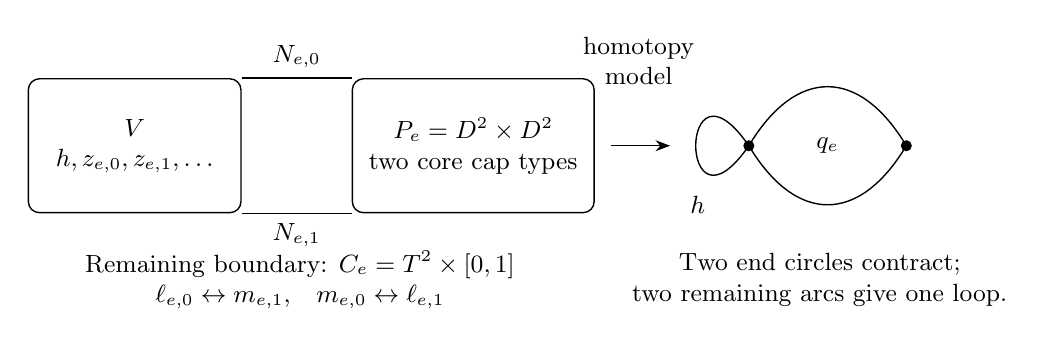
\begin{tikzpicture}[font=\small,>=Stealth,
  block/.style={draw,rounded corners,align=center,inner sep=6pt},
  every path/.style={line width=.5pt}]
  \node[block,minimum width=2.7cm,minimum height=1.7cm] (V) at (0,0)
    {$V$\\$h,z_{e,0},z_{e,1},\ldots$};
  \node[block,minimum width=2.4cm,minimum height=1.7cm] (P) at (4.3,0)
    {$P_e=D^2\times D^2$\\two core cap types};
  \draw (V.north east) -- node[above,sloped] {$N_{e,0}$} (P.north west);
  \draw (V.south east) -- node[below,sloped] {$N_{e,1}$} (P.south west);
  \node[align=center] at (2.1,-1.7)
    {Remaining boundary: $C_e=T^2\times[0,1]$\\
     $\ell_{e,0}\leftrightarrow m_{e,1}$,\quad
     $m_{e,0}\leftrightarrow\ell_{e,1}$};
  \draw[->] (6.05,0) -- (6.8,0);
  \node[above,align=center] at (6.4,.65) {homotopy\\model};
  \fill (7.8,0) circle (2pt);
  \fill (9.8,0) circle (2pt);
  \draw (7.8,0) .. controls (8.4,1) and (9.2,1) .. (9.8,0);
  \draw (7.8,0) .. controls (8.4,-1) and (9.2,-1) .. (9.8,0);
  \draw (7.8,0) .. controls (6.9,1.3) and (6.9,-1.3) .. (7.8,0);
  \node at (7.15,-.75) {$h$};
  \node at (8.8,0) {$q_e$};
  \node[align=center] at (8.7,-1.7)
    {Two end circles contract;\\two remaining arcs give one loop.};
\end{tikzpicture}

\caption{Incidence and peripheral data for one special edge.  This is
a gluing schematic, not a drawing of an embedding of the four-manifold
in three-dimensional space.  The Hopf exterior interchanges longitude
and meridian; the ball kills two end generators and contributes the
single graph loop $q_e$.}\label{geo:fig-graph}
\end{figure}

\subsection{The word list and capped stages}

Write $[u,v]=uvu^{-1}v^{-1}$ and $z^c=czc^{-1}$.  Let $F_h$ be
free on the three named generators $h_0,h_+,h_-$.  Take $\mathcal H$
to be all reduced words of length at most five in
$h_0^{\pm1},h_+^{\pm1},h_-^{\pm1}$, including the empty word.
This is a finite set closed under inversion and reversal.  Put
\[
                  \mathcal R=(\mathcal E\times\mathcal H)^3.
\]
Thus $k=|\mathcal R|=(2d\,|\mathcal H|)^3$ is finite.  The entry
$r=((a,c_1),(b,c_2),(c,c_3))$ specifies the word
\begin{equation}\label{geo:relations}
 R_r=[z_a^{c_1},[z_b^{c_2},z_c^{c_3}]].
\end{equation}
All triples occur, including repetitions, and the three conjugators vary
independently.

We realize each $R_r$ by two punctured tori.  The base $B_r$ has
basis curves $\alpha_r,\beta_r$: the first receives a cap of end type
$a$, while the second receives a punctured torus $S_r$ for the inner
commutator.  Its basis curves $x_r,y_r$ receive caps of end types $b,c$.
Compressing $S_r$ with two copies of its $x_r$ cap will provide the
contracting disc used to construct a dual sphere.  We retain the unused
$y_r$ cap as well; it will identify the group-ring labels of paired
intersections in the exterior of the bases.

A \emph{body} means one of these embedded punctured tori, excluding its
caps.  Bodies and their attaching collars will be disjoint except at
the prescribed attachments.  Opposite end cap types are allowed to
cross in $P_e$.  We first explain how the ribbon construction controls
the attachment framings, then assemble the finite word list.

\begin{lemma}[The framed ribbon operation]\label{geo:framing}
Given two disjoint oriented framed knots in the interior of $Q$ and a
relative path class joining them, one can construct a punctured torus
in a level of a collar $Q\times[0,\epsilon)$ whose two basis curves
resolve normally to these knots.  Its oriented boundary represents
their commutator, with the change of basing given by the chosen path.
The two band framings can be varied by arbitrary integers independently.
The resolved knots admit disjoint rising annuli to the given framed
knots, and a unit band twist changes the relative oriented normal
framing of its annulus by a unit integer.
\end{lemma}

\begin{proof}
Represent the path by an embedded arc disjoint from the knots except
at its endpoints.  Along a narrow finger following this arc move a
short strand of the second knot to the first, stopping when the two
strands meet transversely in a small two-dimensional patch.  Before
the final contact the move is an isotopy.  Thicken the resulting
crossed graph to an oriented ribbon with alternating cyclic order
of the four half-edges at the crossing.  Its regular neighborhood is
a punctured torus.  Choose the normal resolution determined by the
pre-contact strands.  Reversing that specific finger isotopy recovers
the original two-component link.  The boundary traverses the circuits
in the order
$uvu^{-1}v^{-1}$, after a choice of orientation and basing.  The two
sides of the finger insert precisely the chosen change-of-basing
path and its inverse.

The ribbon away from the crossing consists of separate bands.
Insert full twists in either band, supported in a short segment away
from the crossing and the other band.  Take its supporting tube disjoint
from the other resolved knot as well.  Shrinking the displacement in this tube gives
an ambient isotopy of the resolved link that fixes its other component.
Thus a twist preserves the chosen two-component resolution, including
its linking.  The lateral ribbon vector rotates once per full twist,
giving independent integer changes to the two knot framings.

Here is the normal-bundle calculation needed to transfer that integer
to a cap attachment.  Let $t$ be tangent to a basis curve, $b$ its
lateral ribbon vector, $n$ the normal to the ribbon in the level
three-manifold, and $v$ the positive collar direction.  A rising
annulus initially has tangent plane spanned by $t$ and
$r=a n+c v$, with $a^2+c^2=1$ and $c>0$.  Set $w=c n-a v$.
Its oriented normal quotient has frame $([b],[w])$.  Subtracting
the $v$ component divided by $c$ times $r$ identifies this quotient
with the normal plane of the movie knot in the level slice, and gives
\begin{equation}\label{geo:normal-quotient}
 [b]\longmapsto[b],\qquad [w]\longmapsto[n/c].
\end{equation}
Thus it carries exactly the ribbon framing, with a positive rescaling
of the second vector.  During one band twist the pair changes to
\[
 b_\theta=\cos\theta\,b+\sin\theta\,n,
 \qquad n_\theta=-\sin\theta\,b+\cos\theta\,n,
\]
where $\theta$ makes a full turn.  Equation~\eqref{geo:normal-quotient}
has degree one in the oriented rank-two frame group, up to the chosen
sign convention.  This is an integer calculation in
$\pi_1(\operatorname{GL}^+(2,\mathbb R))$, rather than a calculation
of the parity of an ambient three-frame.

The separation of the attaching annuli can be checked in local collar
coordinates $(x,y,n,v)$, with the body in $n=v=0$ and its basis curves
the $x$- and $y$-axes.  Choose the signs of these coordinates to match
the selected normal resolution, and take the initial annuli to be
\[
 (x,0,s,s),\qquad (0,y,-s,s),\qquad s\geq0.
\]
They meet on the body at $s=0$ and are disjoint for $s>0$.  At a small
positive level they give the chosen normal resolution; continue them
by the inverse finger isotopy of the whole link.  The band-twist
isotopies just described are supported away from the other component,
so their traces also preserve this disjointness.
Figure~\ref{geo:fig-ribbon} separates the body coordinates from the
normal coordinates in this local model.  Along a rising movie the same
quotient identification transports the framing to the given knot.
Consequently a full band twist changes by one the obstruction to
extending a prescribed ordered normal frame over an upper cap disc.
Killing that integer extends both vectors: an extended nonzero first
vector and its oriented quarter-turn give a frame, whose second
vector can be adjusted at the boundary through positive independent
vectors.  This also explains why the statement controls a prescribed
boundary framing, not just abstract triviality of a disc bundle.
\end{proof}

\begin{figure}[tb]
\centering
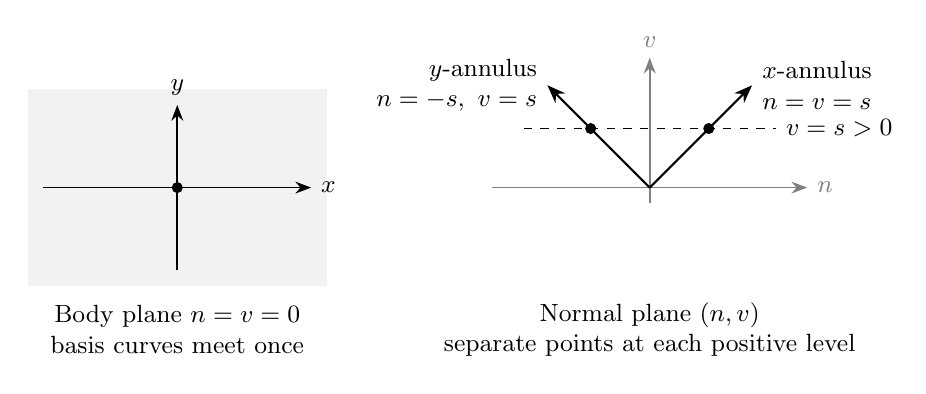
\begin{tikzpicture}[font=\small,>=Stealth,
  every path/.style={line width=.6pt}]
  \begin{scope}[shift={(0,0)}]
    \fill[gray!10] (-1.9,-1.25) rectangle (1.9,1.25);
    \draw[->] (-1.7,0) -- (1.7,0) node[right] {$x$};
    \draw[->] (0,-1.05) -- (0,1.05) node[above] {$y$};
    \fill (0,0) circle (2pt);
    \node[align=center] at (0,-1.8)
      {Body plane $n=v=0$\\basis curves meet once};
  \end{scope}
  \begin{scope}[shift={(6,0)}]
    \draw[->,gray] (-2,0) -- (2,0) node[right] {$n$};
    \draw[->,gray] (0,-.2) -- (0,1.65) node[above] {$v$};
    \draw[->,thick] (0,0) -- (1.3,1.3)
      node[right,align=left] {$x$-annulus\\$n=v=s$};
    \draw[->,thick] (0,0) -- (-1.3,1.3)
      node[left,align=right] {$y$-annulus\\$n=-s,\ v=s$};
    \draw[dashed] (-1.6,.75) -- (1.6,.75);
    \fill (-.75,.75) circle (2pt);
    \fill (.75,.75) circle (2pt);
    \node[anchor=west,inner sep=2pt] at (1.65,.75) {$v=s>0$};
    \node[align=center] at (0,-1.8)
      {Normal plane $(n,v)$\\separate points at each positive level};
  \end{scope}
\end{tikzpicture}

\caption{Local coordinates for the ribbon attachment.  The left panel
shows the intersecting basis curves in the body plane; the right panel
shows their distinct rising rays in the normal $(n,v)$-plane.  At each
positive collar level the two annuli are separated in $n$.  The chosen
resolution is the one recovered by reversing the pre-contact finger
isotopy.  This local picture makes no assertion that cap images are
mutually disjoint.}\label{geo:fig-ribbon}
\end{figure}

\begin{lemma}[Simultaneous capped stages]\label{geo:stages}
For every $r\in\mathcal R$ there is a punctured torus $B_r$ properly
embedded in $V$, with boundary a knot in $\operatorname{int}Q$.
The $B_r$ are mutually disjoint.  They have intersecting basis curves
$\alpha_r,\beta_r$ and the following attachments in $G$:
\begin{enumerate}
\item A shallow cap at $\alpha_r$ ends in a separate parallel copy of
the core disc of end $a$.
\item A further punctured torus $S_r$ is attached at $\beta_r$.
Its basis curves $x_r,y_r$ have caps of end types $b,c$, respectively.
Its boundary, with the prescribed basing, represents
$[z_b^{c_2},z_c^{c_3}]$, and $\partial B_r$ represents $R_r$.
\item Compressing $S_r$ along $x_r$ with two framed parallels of its
cap produces an embedded disc $D_r$.  Intersections of $D_r$ with
other objects are allowed.  The extension of $D_r$ towards $\beta_r$
has a framing that extends the angular normal-circle vector required
to compress $\beta_r\times S^1$.
\end{enumerate}
Except at the intended attachments, every body and attaching collar
is disjoint from every other such piece.  All other intersections
are transverse crossings of opposite end cap sheets in the product
charts \eqref{geo:product-sheets}.
\end{lemma}

\begin{proof}
Give each leaf occurrence its own parallel longitude knot on the
$Q$ side of its end torus, even when several occurrences have the
same label.  Reserve a separate return lane inside the corresponding
solid torus.  Each lane leads to its own framed core-disc parallel
in $P_e$.  There are finitely many occurrences, so all lanes may be
chosen disjoint within each end family.

Choose narrow, separated ranges of collar levels centered at
\[
                    0<t_B<t_S<t_T<\epsilon.
\]
The base-body operations occupy the range about $t_B$, the inner-body
operations the range about $t_S$, and the transfers into the end solid
tori the range about $t_T$.  Each body-operation range includes room
above its body level for the rising resolution and inverse finger isotopy of
Lemma~\ref{geo:framing}.  Between ranges, continuing knots run in narrow
disjoint pipes; at an active range all inactive continuations remain in
their pipes.

To trace one relation through these heights, its base boundary rises
from level zero to $B_r$ near $t_B$.  The shallow attachment at
$\alpha_r$ continues to the transfer range.  The other attachment rises
from $\beta_r$ to the boundary of $S_r$ near $t_S$; the two attachments
at $x_r,y_r$ then rise through their own pipes to the transfer range.
There every leaf moves from the $Q$ side into its end solid torus and
returns down its reserved lane in the torus interior to its cap in $P_e$.
These downward lanes lie outside the $Q$-side body neighborhoods.
The construction order is upper stage first: after making $S_r$, we
carry its boundary down to a handoff knot at the upper side of the
base-operation range.  With this knot and the slot-$1$ leaf fixed above
the lower body level, we choose their connecting arc.  The lower
ribbon's rising movie then joins the body to those two inputs.  Thus the
later base operation is below the earlier upper body and avoids the
inactive leaf pipes.

For either body-operation range, once its input knots have been fixed,
choose the connecting arcs with separate endpoints and the prescribed relative
path classes in $Q$.  General position in this three-manifold makes
the finitely many arcs embedded, mutually disjoint and disjoint from
the other knots.  No prescribed path class in a fixed link complement
is needed.  Small neighborhoods of these graphs accommodate the
ribbons, isotopies and local twists.

Choose the connecting arcs for the slot-$2,3$ pairs as disjoint arcs
in $Q$, and first apply Lemma~\ref{geo:framing} to every pair of leaf
occurrences in slots $2,3$, to make $S_r$, avoiding all slot-$1$ leaf knots.
Attach the rising annuli to the leaf knots, and match the $x_r$ band
framing to the framed $x_r$ cap.  Cutting out an annulus along $x_r$
leaves a pair of pants.  Capping its two new boundary circles by
nearby copies of the $x_r$ cap gives a disc $D_r$.  The extended
lateral normal field supplied by Lemma~\ref{geo:framing} places
the two copies at the cut band sides.  This disc is embedded:
the retained body and its collars are disjoint, and the only cap
pieces retained have the same end type.  In particular, crossings
with the unused $y_r$ cap or with another leaf are not self-crossings
of $D_r$.

Return the boundary knot of $S_r$ along an attaching collar to a
lower level.  Its contracting disc supplies a normal-framing class
at this handoff.  With the returned boundary knots now fixed, choose
the lower connecting arcs and pair each knot with its slot-$1$ leaf, again by
Lemma~\ref{geo:framing}, to make $B_r$.  Choose the
$\beta_r$ band twist so that the transported ordered frame extends
over this already constructed contracting disc.  At the chosen
normal phase of $\beta_r\times S^1$, the vector $w$ in
\eqref{geo:normal-quotient} is its angular tangent.  Extension of
the ordered frame therefore extends this particular angular
vector, as required for compression of the product torus.

These choices are sequential.  If $n_x,n_\beta$ are the two twists,
the two relative framing obstructions have the form
\[
 o_x(n_x,n_\beta)=o_x(0,0)+\varepsilon_x n_x,
 \qquad
 o_\beta(n_x,n_\beta)=o_\beta(n_x,0)
                           +\varepsilon_\beta n_\beta,
 \qquad \varepsilon_x,\varepsilon_\beta\in\{1,-1\}.
\]
The lower $\beta_r$ twist does not change the fixed upper disc or
its $x_r$ framing.  One first sets $o_x=0$, records the resulting
handoff framing, and then sets $o_\beta=0$.  There is no simultaneous
parity assumption hidden in these choices.

Chosen changes of basing make the leaf circuits the conjugates in
\eqref{geo:relations}.  Applying the commutator rule first to $S_r$
and then to $B_r$ gives the asserted words.  Paths recording basings
need not themselves be physical attachments from a single basepoint.

Finally extend the base boundaries down to level zero in $Q$.
This makes the $B_r$ proper in $V$.  Choose the remaining small
parallel displacements and radii after all finitely many bodies
and collars have been fixed.  Outside the attachment charts and
the cap-crossing charts their compact disjoint pieces have positive
separation; inside the charts use the product choices
\eqref{geo:product-sheets}.  This gives simultaneous smooth choices
with exactly the asserted intersections.
\end{proof}

\subsection{The exterior, the dual spheres, and their labels}

Delete small open relative tubular neighborhoods of the bases only:
\begin{equation}\label{geo:exterior}
 M=\overline{G\setminus\bigcup_{r\in\mathcal R}
                                      \nu(B_r)}.
\end{equation}
The relative neighborhoods meet $\partial G$ in the corresponding
boundary-knot neighborhoods.  Choose their radii small enough to
miss every upper-stage piece except its prescribed initial
attachment.  Round corners with compatible collars.  This is a
compact oriented smooth four-manifold with nonempty boundary.
It is connected: paths may be moved off finitely many embedded
surfaces in dimension four, and the complement of the surfaces
retracts radially onto the exterior of sufficiently small tubes.

Truncate each shallow cap at the boundary of the corresponding
base tube and call the resulting proper disc $f_r$.  Its boundary
circles are mutually disjoint smooth embeddings in $\partial M$.
The cap construction gives smooth disc maps, made generic while
keeping the product collars fixed.  In fact each individual disc
is embedded; discs of opposite end types may meet one another.
Their normal bundles supply their induced boundary framings.

At a slightly larger radius than the deleted tube, put
\[
 T_r=\beta_r\times S^1\ \subset M.
\]
This product torus meets the shallow attaching annulus at exactly
one transverse point, since $\alpha_r$ and $\beta_r$ cross once.
At the distinct phase used by the further stage, compress $T_r$
along its $\beta_r$ direction using two parallels of the extended
contracting disc $D_r$.  Denote the resulting sphere by $g_r$.
Figure~\ref{geo:fig-stages} distinguishes the two successive pairs of
cap copies in this sphere.

\suppressfloats[t]
\begin{figure}[!ht]
\centering
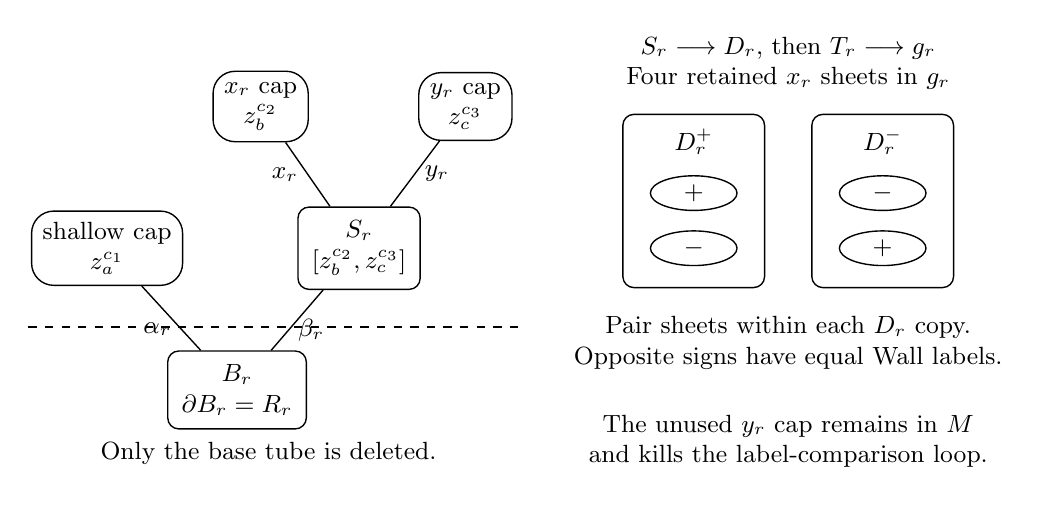
\begin{tikzpicture}[font=\small,>=Stealth,
  body/.style={draw,rounded corners,align=center,inner sep=5pt},
  capnode/.style={draw,rounded corners=8pt,align=center,inner sep=4pt},
  every path/.style={line width=.5pt}]
  \node[body] (base) at (0,0) {$B_r$\\$\partial B_r=R_r$};
  \node[capnode] (shallow) at (-1.65,1.8) {shallow cap\\$z_a^{c_1}$};
  \node[body] (upper) at (1.55,1.8) {$S_r$\\$[z_b^{c_2},z_c^{c_3}]$};
  \node[capnode] (x) at (.3,3.6) {$x_r$ cap\\$z_b^{c_2}$};
  \node[capnode] (y) at (2.9,3.6) {$y_r$ cap\\$z_c^{c_3}$};
  \draw (base) -- node[pos=.33,left] {$\alpha_r$} (shallow);
  \draw (base) -- node[pos=.33,right] {$\beta_r$} (upper);
  \draw (upper) -- node[left] {$x_r$} (x);
  \draw (upper) -- node[right] {$y_r$} (y);
  \draw[dashed] (-2.65,.8) -- (3.6,.8);
  \node[align=center] at (.4,-.8) {Only the base tube is deleted.};

  \node[align=center] at (7,4.15)
    {$S_r\longrightarrow D_r$, then $T_r\longrightarrow g_r$\\
     Four retained $x_r$ sheets in $g_r$};
  \draw[rounded corners] (4.9,1.3) rectangle (6.7,3.5);
  \draw[rounded corners] (7.3,1.3) rectangle (9.1,3.5);
  \node at (5.8,3.15) {$D_r^{+}$};
  \node at (8.2,3.15) {$D_r^{-}$};
  \draw (5.8,2.5) ellipse (.55 and .22);
  \draw (5.8,1.8) ellipse (.55 and .22);
  \draw (8.2,2.5) ellipse (.55 and .22);
  \draw (8.2,1.8) ellipse (.55 and .22);
  \node at (5.8,2.5) {$+$};
  \node at (5.8,1.8) {$-$};
  \node at (8.2,2.5) {$-$};
  \node at (8.2,1.8) {$+$};
  \node[align=center] at (7,.6)
    {Pair sheets within each $D_r$ copy.\\
     Opposite signs have equal Wall labels.};
  \node[align=center] at (7,-.65)
    {The unused $y_r$ cap remains in $M$\\
     and kills the label-comparison loop.};
\end{tikzpicture}

\caption{Attachment tree for one relation and the two ordered
compressions.  The left panel records attachments; the right panel
separates the two outer contracting-disc copies and their inner cap pairs.
Signs indicate the opposite induced orientations in each pair.
Opposite end cap types may cross in the balls $P_e$.  The unused $y_r$ cap
remains in the manifold and will kill the comparison loop in
Lemma~\ref{geo:labels}.}\label{geo:fig-stages}
\end{figure}

\begin{lemma}[Embedded framed dual candidates]\label{geo:dual-candidates}
Each $g_r$ is individually embedded and has trivial normal bundle.
It follows that
\[
 \lambda(g_r,g_r)=0,\qquad \widetilde\mu(g_r)=0.
\]
The compression leaves the single product-torus intersection
with $f_r$ unchanged.  Every other intersection involving an
$f_r$ and a $g_s$, or two distinct spheres, occurs on the cap
sheets in \eqref{geo:product-sheets}.
\end{lemma}

\begin{proof}
The chosen angular normal field extends over the embedded disc
$D_r$, so a narrow interval thickening of that disc replaces the
annulus on $T_r$ by its two disjoint parallel boundary discs.
Away from the attaching curve the thickening misses $T_r$ if
it is sufficiently small.  All cap sheets in this one sphere
come from its own $x_r$ cap and hence have the same end type.
The disjoint-body construction and the local surgery model give
embeddedness.  The phase containing the shallow-cap intersection
is disjoint from the annulus being replaced, so that point remains.
The separation choices in Lemma~\ref{geo:stages} account for all
other possible intersections.

The interval thickening is an oriented three-chain in $M$ whose
boundary is the difference between the original annulus and the
two replacement discs.  Consequently $[g_r]=[T_r]$ in
$H_2(M;\mathbb Z)$, up to a harmless orientation sign.  The torus
has an explicit trivial normal bundle, with one vector lateral
to $\beta_r$ in the base and one vector radial in the normal
disc to the base.  Thus its ordinary self-intersection is zero.
Homology invariance of that pairing gives $g_r\cdot g_r=0$.
For an embedded oriented sphere this is the Euler number of its
oriented normal plane bundle.  Such a bundle on $S^2$ is classified
by its Euler number, so $g_r$ has a disjoint normal pushoff.
The pushoff computes zero in the full group-ring diagonal pairing.
Embeddedness gives no double points at all in the Wall invariant,
and in particular gives the stated reduced invariant.
\end{proof}

Opposite intersection signs do not suffice for the off-diagonal
calculations: their labels must agree in $\pi_1(M)$, not merely
in $\pi_1(G)$.  The unused cap in each upper stage supplies this
extra assertion.

\begin{lemma}[Cancellation in the exterior]\label{geo:labels}
Within one contracting-disc copy on a sphere, pair the two
oppositely oriented $x$-cap sheets at their crossings with any
fixed opposite-type sheet.  The paired intersections have equal
Wall labels in $\pi_1(M)$ and opposite signs.  All cap-sheet
contributions to $\lambda(f_r,g_s)$ and to
$\lambda(g_r,g_s)$ for $r\ne s$ therefore cancel.
\end{lemma}

\begin{proof}
Use the product attachment collars to make the carrier and its
comparison homotopy explicit in the exterior.  Choose a common small
radius $\varepsilon$ for the deleted base tubes, smaller than all the
finitely many collar lengths.  Take $T_s$ at radius $2\varepsilon$.
Shorten the initial collar of $S_s$ at radius $3\varepsilon$ and join
it back to $T_s$ by the radial annulus between these two radii; call
this retained upper stage $S_s$ as well.  This collar shortening
changes neither its two basis curves nor its fundamental group.
All caps are retained.  Choose subsequent parallel displacements
smaller than $\varepsilon/10$ and than the positive clearances from
the other deleted tubes.  The cap-parallel collapse and the band
comparison below can be fixed on this radial collar, so their images
stay outside every deleted tube.

For this retained upper stage of entry $s$ form the abstract complexes
\[
 K_x=S_s\cup_{x_s}D_x,\qquad
 K=S_s\cup_{x_s}D_x\cup_{y_s}D_y.
\]
Attaching annuli are included in the cap notation.  The actual
configuration gives a map $j:K\longrightarrow M$ with the
collar just specified.  The caps may cross other cap images;
none of those images has been deleted from $M$.  The presentations
\begin{equation}\label{geo:carrier-groups}
 \pi_1(K_x)=\langle x_s,y_s\mid x_s\rangle
               =\langle y_s\rangle,
 \qquad
 \pi_1(K)=\langle x_s,y_s\mid x_s,y_s\rangle=1
\end{equation}
are presentations of these abstract complexes.

Collapse the small parallel displacement in the compressed disc
$D_s$ and reglue its cut $x_s$ band.  This gives a map
$c:D_s\longrightarrow K_x$ identifying corresponding points
of its two cap copies with the same point of $D_x$.  The actual
map of $D_s$ into $M$ is homotopic to $j\circ c$ by the normal
intervals of its cap parallels and the matching band collars.
The homotopy stays in a neighborhood of the upper stage, away
from every deleted base tube.  It is a homotopy of maps and is
allowed to cross the other cap images.

Fix one of the two outer copies of $D_s$ in $g_s$.  From a point
on its retained upper body choose paths $\gamma_+,\gamma_-$
to corresponding crossings on its two inner cap sheets.  In a
crossing chart these sheets and the fixed other sheet are
\[
 D^2\times\{a_+\},\quad D^2\times\{a_-\},
                 \quad \{b\}\times D^2.
\]
The short comparison path
$\tau(u)=(b,(1-u)a_++u a_-)$ is simultaneously a path on the
fixed other sheet and the normal interval between the paired
cap points.  Choose the paths on the fixed sheet using this
segment.  Up to conjugation by the common path from the sphere's
whisker, the quotient of the two Wall labels is represented by
\[
                  \gamma_+\,\tau\,\gamma_-^{-1}.
\]
Under the collapse comparison this becomes
$c(\gamma_+)c(\gamma_-)^{-1}$ in $K_x$: the segment $\tau$
collapses to the single point of $D_x$.  The loop might represent
a nonzero power of $y_s$ in $K_x$; Equation~\eqref{geo:carrier-groups}
kills it in $K$, using the actual unused $y_s$ cap.  Composing
its nullhomotopy with $j$ proves equality of the labels in $M$.
Arbitrary conjugators are already part of the attaching paths;
they do not alter the simple connectivity of $K$.

The two inner cap copies cap the two boundary components of the
annulus cut from $S_s$, so have opposite induced orientations.
Their signs against any fixed sheet are therefore opposite.
Reversing the orientation of an outer contracting-disc copy
reverses both signs and preserves this conclusion.  Apply the
pairing separately within each outer copy, and separately for
each fixed cap sheet on the other surface.  This accounts for
every cap crossing, including repeated end labels and opposite
end labels within one entry.  In particular no comparison of
paths between the two outer phases, and no contraction of a
base meridian in $M$, has been used.
\end{proof}

\begin{corollary}[The exact algebraic input]\label{geo:input-invariants}
There are orientations and whiskers for the discs and spheres such
that, for all $r,s\in\mathcal R$ and
$R=\mathbb Z[\pi_1(M)]$,
\begin{equation}\label{geo:invariants}
 \lambda(f_r,g_s)=\delta_{rs}\,1\in R,
 \qquad \lambda(g_r,g_s)=0\in R,
 \qquad \widetilde\mu(g_r)=0.
\end{equation}
In particular the normal second Stiefel--Whitney number of every
$g_r$ is zero.  These data satisfy all algebraic and boundary
hypotheses of the unrestricted disc-embedding assertion.
\end{corollary}

\begin{proof}
Lemmas~\ref{geo:dual-candidates} and~\ref{geo:labels} leave exactly
one signed group element in $\lambda(f_r,g_r)$ and no other
contributions.  Orient $g_r$ and change its whisker so that this
coefficient is $+1$.  Whisker changes multiply or conjugate zero
entries by units and hence preserve the other vanishings.
Triviality of the normal bundles proves the Stiefel--Whitney
assertion.  The manifold is oriented, so its orientation character
is trivial and the involution on $R$ is $h\mapsto h^{-1}$.
The reduced Wall invariant vanishes even before imposing its
additive relations $h-h^{-1}$ and the identity coefficient.
The discs have disjoint embedded boundary circles and the proper
collar model.  There is no requirement to make their mutual
intersections or self-intersection invariants vanish.
\end{proof}

\subsection{Topological disc images give smooth cuts}

\begin{lemma}[Moving the graph map off the protected discs]
\label{geo:topological-cuts}
Suppose there are pairwise disjoint proper locally flat embeddings
$\overline f_r:D^2\longrightarrow M$ with
$\overline f_r|_{S^1}=f_r|_{S^1}$.  Then $p_0$ is homotopic,
relative to $\partial G$, to a map $p:G\longrightarrow\Gamma$
with the following properties.  The bases, the short return
annuli in their deleted tubes, and the disc images lie in
$p^{-1}(\Gamma_h)$.  For one interior point of each $q_e$ edge,
the inverse image $J_e$ is a compact smooth oriented
three-manifold with exactly one boundary torus.  Additional
closed components of $J_e$ are allowed.
\end{lemma}

\begin{proof}
Join the boundary of each actual embedded disc back to
$\alpha_r$ by the radial annulus in the deleted base tube.
The bases and these return annuli lie in $V$ and hence already
map into $\Gamma_h$.  The boundary map of each disc lies in
$\Gamma_h$ and is nullhomotopic in $\Gamma$ because the actual
disc gives a filling.  The inclusion
$\pi_1(\Gamma_h)\longrightarrow\pi_1(\Gamma)$ is injective,
so it has a filling in $\Gamma_h$.  The original filling and
this new filling are homotopic relative boundary since
$\pi_2(\Gamma)=0$.  Transfer this homotopy to the disc image
using the embedding parametrization.  This step uses no
homotopy between an output disc and its input cap.

Let $B$ be the union of the bases, return annuli, and disc
images, and put $A=B\cup\partial G$.  Prescribe the just
constructed homotopies on the discs and keep the other parts
fixed.  These prescriptions agree on intersections: disc
boundaries are fixed, disc interiors are mutually disjoint and
proper in $M$, and the only intersections with the returned
pieces are the stated attaching circles.  Pasting finitely
many compact closed sets gives a continuous homotopy on $A$.
Only $B$ is to map into $\Gamma_h$; the $q$-collar portions
of $\partial G$ keep their prescribed product values.

Here the extension to $G$ need not assume that the topological
disc images are smooth or that their inclusion is a cofibration.
A finite graph is an absolute neighborhood retract for metric
spaces.  Apply its neighborhood-extension property to the
prescribed map on the closed subset
\[
       (G\times\{0\})\cup(A\times[0,1])\ \subset G\times[0,1].
\]
It extends to an open neighborhood $O$ of that subset.  Compactness
of $A\times[0,1]$ gives a neighborhood $U$ of $A$ with
$U\times[0,1]\subset O$.  Choose a continuous function
$\chi:G\longrightarrow[0,1]$ equal to one on $A$ and supported
in $U$.  If $\widetilde H$ is the neighborhood extension, then
\[
             H(x,t)=\widetilde H(x,\chi(x)t)
\]
is defined on all of $G\times[0,1]$: when $\chi(x)>0$ it uses
$U\times[0,1]$, and otherwise it uses the time-zero slice.
It is the required extension, fixed on $\partial G$.  Its final
map sends $B$ into $\Gamma_h$.

Choose mutually disjoint small open intervals about the midpoints
of the $q_e$ edges.  Their closed smaller intervals miss
$\Gamma_h$, so their inverse images miss the protected compact
set $B$.  On $\partial G$ the map is already the fixed coordinate
on the single collar $C_e=T^2\times[0,1]$.  In a small boundary
collar straighten its real interval coordinate to be constant
in the inward normal direction, using an interpolation fixed
on the boundary.  Use a slightly larger target interval to
localize this operation away from $B$.  Relative smooth
approximation of real functions, followed by relative
transversality in the remaining interior, makes the map smooth
and transverse near a smaller middle level, preserving the
boundary product and staying off $B$.  The intervals for
different edges have disjoint supports.  These changes are
homotopies within intervals, so the resulting $p$ is still
homotopic to $p_0$ relative boundary. The regular-value and boundary
regular-fiber statements are those of \cite[Section~2, pp.~10--13]{Milnor1965};
the fixed product collar supplies regularity on the boundary.

Each level $J_e$ is therefore a compact smooth hypersurface,
cooriented by the interval and oriented by $G$.  Its boundary
is exactly the boundary level $T^2\times\{\mathrm{point}\}$
in $C_e$; $Q$ contributes no boundary point at that level.
There is one component with this boundary torus, and every
other component is closed.  All the topological disc images
and returned pieces remain disjoint from the cuts.
\end{proof}

For the deformation argument, fix the following reference representation
of the $h$-subgroup, with $\mathfrak l=\mathfrak{sl}_2(\mathbb C)$:
\begin{equation}\label{geo:matrices}
 \rho(h_0)=\begin{pmatrix}2&0\\0&1/2\end{pmatrix},\qquad
 \rho(h_+)=\begin{pmatrix}1&1\\0&1\end{pmatrix},\qquad
 \rho(h_-)=\begin{pmatrix}1&0\\1&1\end{pmatrix}.
\end{equation}
The length-five word set $\mathcal H$ was chosen so that the operators
$\operatorname{Ad}\rho(c)$ for $c\in\mathcal H$ span
$\operatorname{End}(\mathfrak l)$; the calculation is given
at its point of use in Lemma~\ref{geo:spanning}.

\begin{proposition}[The geometric input and the forced cut data]
\label{geo:construction}
For every $d\geq5$, with the finite word set $\mathcal H$ defined above,
the preceding construction produces
a compact connected oriented smooth four-manifold $M$ with
nonempty boundary, a finite family $F=(f_r)_{r\in\mathcal R}$
of smooth proper disc maps with disjoint embedded boundary,
and individually embedded framed sphere maps
$(g_r)_{r\in\mathcal R}$ satisfying \eqref{geo:invariants}.

If the circles $\partial F$ bound pairwise disjoint proper
locally flat embedded discs in $M$, the following data exist:
\begin{enumerate}
\item The compact oriented smooth four-manifold $G$ has a
homotopy equivalence $p:G\longrightarrow\Gamma$, where
$\Gamma$ is the rose on $h_0,h_+,h_-,q_1,\ldots,q_d$.
The boundary is $Q\cup\bigcup_e C_e$, with the free group
and peripheral coordinates of Lemma~\ref{geo:graph} and the
longitude--meridian interchange \eqref{geo:hopf-collar}.
\item There are disjoint cooriented smooth cuts $J_1,\ldots,J_d$,
each a compact oriented three-manifold with one boundary torus
and possibly additional closed components.  Their boundary
tori are the fixed product cuts in the $C_e$.
\item Cutting $G$ along all $J_e$ gives a compact oriented smooth
four-manifold $X$, possibly disconnected.  With half collars
absorbed into $Q$, its boundary is obtained by gluing $Q$ to
the two oppositely oriented copies of each $J_e$ along their
boundary tori.  Every torus-bearing wall component has just
that one torus; closed wall components remain separate.
Regluing the paired cuts recovers $G$.
\item The map on $X$ lands in the graph cut open at the chosen
$q_e$ points, namely $\Gamma_h$ with the resulting half-edges;
it is constant on every copy of a cut at its endpoint value.
All words \eqref{geo:relations} are trivial in the fundamental
group of the component $X_Q$ containing $Q$, with the original
basings in $Q$.
\item Extend \eqref{geo:matrices} to $\pi_1(\Gamma)$ by
$\rho(q_e)=1$.  The associated adjoint local system on $G$
restricts to $\rho$ on the $h$ generators, to the identity on
all $z_a$, and to a trivial system on each $J_e$, with matching
reference frames on its two copies induced by the graph point.
\end{enumerate}
The implication uses only the asserted embedded discs.  It imposes
neither output-dual conditions nor an additional framing or relative
homotopy condition on those discs.
\end{proposition}

\begin{proof}
The input assertions are Corollary~\ref{geo:input-invariants}.
Use Lemma~\ref{geo:topological-cuts} to obtain $p$ and $J_e$.
Since $p$ is homotopic to $p_0$, Lemma~\ref{geo:graph} makes
it a homotopy equivalence.  Cutting along the disjoint level
hypersurfaces gives the stated collared manifold $X$, whose
corners can be rounded.  Connectedness of $X$ was not used
and is not asserted.  The connected region $Q$ singles out
one component $X_Q$.

For each $r$, the union of $B_r$, its return annulus and its
new disc misses every cut and meets $Q$.  It therefore lies
in $X_Q$.  In that union the curve $\alpha_r$ bounds the
returned disc, so the base boundary, which represents
$[\alpha_r,\beta_r]$, is nullhomotopic.  Its word in $Q$ is
exactly $R_r$, up to the already fixed orientation and basing
conventions.  Any overall conjugate or inverse has the same
nullity, so all based relations in \eqref{geo:relations}
hold in $\pi_1(X_Q)$.  This group argument does not assert
that an entire base has been compressed to an embedded disc.
The map to the cut graph and all the peripheral assertions
follow directly from the fixed product boundary values.
Pullback from the graph gives the last local-system assertion.
\end{proof}

The remaining sections rule out the cut data in
Proposition~\ref{geo:construction}.  Their smoothness comes from
regular levels of the ambient graph map away from the protected disc
images; the hypothetical discs themselves have not been smoothed.

\newpage

\section{Deformations of the cut data}
\label{sec:deformation}

The cut data in Proposition~\ref{geo:construction} have two consequences
for representations near $\rho$: complementary tangent spaces for the
paired wall restrictions, and a cube-zero ideal generated by the end
holonomies minus the identity.  The first comes from the graph homotopy
type of $G$ and the longitude--meridian interchange; the second uses the
triple commutator relations retained in the component $X_Q$.

We use $\Gamma$ and $\Gamma_h$ for the graph and its $h$-subrose.
The coefficient system $\mathfrak l_\rho$ is the pullback of the adjoint
system of \eqref{geo:matrices}, extended by $\rho(q_i)=1$.  It is trivial
on every wall, with matching reference frames on the two copies induced
by the cut point.  The trace form
$(u,v)\mapsto\operatorname{tr}(uv)$ identifies this system with its dual.
Throughout, cohomology of $X$ or $J_i$ includes all components: $X$ need
not be connected, and a wall may have closed components in addition to
its one component with torus boundary.

\subsection{The paired restriction maps}

\begin{lemma}[Paired Mayer--Vietoris maps]
\label{def:paired-mv}
Let
\[
 W_h=\operatorname{im}\bigl(H^1(\Gamma_h;\mathfrak l_\rho)
                 \longrightarrow H^1(X;\mathfrak l_\rho)\bigr).
\]
Here the map uses the retraction of the cut-open graph onto its
\(h\)-rose.  For either degree, write \(r_i^\pm\) for restriction to
the two copies of \(J_i\).  The map
\begin{equation}
 \Delta(u,v)=
  \bigl(r_i^+u-r_i^-v,\ r_i^-u-r_i^+v\bigr)_{i=1}^d
 \label{def:delta}
\end{equation}
is onto in degree one, with kernel \(W_h\oplus W_h\), and is an
isomorphism in degree two.  Consequently, if
\(H^1(X;\mathfrak l_\rho)=W_h\oplus U\), then
\[
 \Delta:U\oplus U\xrightarrow{\ \cong\ }
             \bigoplus_i\bigl(H^1(J_i;\mathfrak l)
                          \oplus H^1(J_i;\mathfrak l)\bigr).
\]
\end{lemma}

\begin{proof}
Take the two-sheeted cover of \(G\) classified by the homomorphism
sending every \(q_i\) to the nontrivial element of \(\mathbb Z/2\)
and every \(h\)-loop to zero.  The lift of \(p\) is a homotopy
equivalence with the corresponding graph cover.  Thus the cover has
zero cohomology in degrees at least two, with the lifted local
system as well as with constant coefficients.  After adjoining
small product collars, its decomposition has two vertex spaces,
both copies of \(X\), and two edge spaces per label, both copies of
\(J_i\).  The pairings go from one vertex copy to the opposite side
of the other, giving exactly \eqref{def:delta}.  The relevant part of
Mayer--Vietoris is
\[
 H^1(\widetilde G)\longrightarrow H^1(X)^{\oplus2}
 \xrightarrow{\Delta}\bigoplus_i H^1(J_i)^{\oplus2}
 \longrightarrow H^2(\widetilde G)=0
\]
and
\[
 0=H^2(\widetilde G)\longrightarrow H^2(X)^{\oplus2}
 \xrightarrow{\Delta}\bigoplus_i H^2(J_i)^{\oplus2}
 \longrightarrow H^3(\widetilde G)=0 .
\]
The omitted coefficients in these two displays are the specified
local systems.

The image in the middle degree-one group is precisely
\(W_h\oplus W_h\).  In one direction, a class restricted from the
graph cover factors on each vertex through its cut-open graph,
and hence through the associated \(h\)-rose.  Conversely, choose
cellular one-cochains representing any two classes on the two
\(h\)-roses.  Extend them to the graph cover by arbitrary values,
for example zero, on the remaining edges.  There are no two-cells,
so the extensions are cocycles.  Their restrictions give the
chosen pair of classes on \(X\).  This argument uses direct sums
over all components of \(X\), and imposes no connectedness
assumption on it.
\end{proof}

\begin{lemma}[Slopes and internal directions]
\label{def:slopes}
The ends of each cut can be designated \(+\) and \(-\), and torus
coordinates \((\theta_i,\eta_i)\) of period one can be chosen, so that
the image of
\[
 H^1(J_i;\mathbb C)\longrightarrow H^1(\partial J_i;\mathbb C)
\]
is the \(\theta_i\)-axis.  In \(Q\), the \(\eta_i\)-circle bounds on
the positive side and the \(\theta_i\)-circle bounds on the negative
side.  Put
\[
 n_i=\dim_{\mathbb C}H^1(J_i,\partial J_i;\mathfrak l),
 \qquad D=\sum_i n_i,
 \qquad
 \mathcal Y=\bigoplus_i(\mathbb C^{n_i}\oplus\mathbb C^{n_i}).
\]
Then \(\dim U=3d+D\).  The joint first-slope restriction
\(U\to\mathfrak l^d\) is onto.  Its kernel \(U_0\) has dimension \(D\).
The two maps from \(U_0\) to \(\mathcal Y\) given by the paired
restrictions and by their interchange are injective and have
complementary images.
\end{lemma}

\begin{proof}
Poincare--Lefschetz duality \cite[Theorem~3.43]{Hatcher2002} and the exact sequence of the pair imply
that the restriction image in the cohomology of the boundary of
an oriented compact three-manifold is its own annihilator for
the intersection form.  For completeness, the connecting map
\(H^1(\partial J_i)\to H^2(J_i,\partial J_i)\) is dual, up to sign,
to the restriction map.  Exactness therefore identifies the
kernel of that connecting map, which is the restriction image,
with the annihilator of that image.  On a single torus a subspace
equal to its annihilator is a line.  Closed components of \(J_i\)
make no contribution to the boundary map.  Denote this line by
\(L_i\).

Tensoring with \(\mathfrak l\) gives the corresponding assertion
for the trivial wall system.  A restriction from the positive or
negative copy of \(X\) has zero evaluation on the slope which
bounds in \(Q\), because the local system is trivial on that
torus.  These two constraints are the distinct coordinate axes
interchanged by the Hopf gluing.  If \(L_i\) were neither axis,
both restrictions would have zero torus value.  This contradicts
surjectivity in Lemma~\ref{def:paired-mv}, since
\(H^1(J_i;\mathfrak l)\) has a nonzero boundary restriction.
Thus \(L_i\) is one axis; designate the contributing end positive
and call this the first slope.

The map \(H^0(J_i;\mathfrak l)\to
H^0(\partial J_i;\mathfrak l)\) is onto: constants on the unique
component with boundary suffice.  The exact sequence consequently
identifies
\begin{equation}
 H^1(J_i,\partial J_i;\mathfrak l)
 \ \cong\
 \ker\bigl(H^1(J_i;\mathfrak l)
                  \longrightarrow H^1(\partial J_i;\mathfrak l)\bigr).
 \label{def:relative-identification}
\end{equation}
These are the \(n_i\) internal directions, including all degree-one
cohomology of every closed component.  They pair perfectly with
\(H^2(J_i;\mathfrak l)\) by integration and the trace form.
In particular \(\dim H^1(J_i;\mathfrak l)=3+n_i\).

The isomorphism in Lemma~\ref{def:paired-mv} now gives
\(\dim U=3d+D\).  Its first-slope coordinates are the first-slope
values of \(u\), and the negatives of those of \(v\), because all
opposite-side values are zero.  Surjectivity implies independent
surjectivity onto the \(3d\) first-slope coordinates.  On their
kernel the same isomorphism becomes
\[
 U_0\oplus U_0\longrightarrow\mathcal Y,\qquad
 (u,v)\longmapsto R(u)-\sigma R(v),
\]
where \(R\) is paired restriction and \(\sigma\) interchanges the
two slots for each \(i\).  This proves the last assertions.
\end{proof}

\subsection{Finite algebraic equation charts}

From now on orient \(J_i\), including each of its closed components,
as its positive copy in the oriented boundary of \(X\).  Its
negative copy then has the opposite orientation.

\begin{definition}[Scalar rings and formal coefficients]
\label{def:coefficient-convention}
An algebraic parameter chart will mean a local \(\mathbb C\)-algebra
essentially of finite type and etale over an affine coordinate
space at the designated origin.  Its completion is
\(B=\mathbb C[[v_1,\ldots,v_N]]\), with maximal ideal \(\mathfrak m\).
Finite collections of algebraic germs obtained by an implicit
equation with invertible Jacobian can always be placed in one such
chart, after replacing it by a common etale neighborhood.

For a smooth manifold \(Z\), smooth forms with formal coefficients
mean
\[
 \Omega^j(Z)\widehat\otimes B
   =\varprojlim_k\bigl(\Omega^j(Z)\otimes_{\mathbb C}
                                     B/\mathfrak m^k\bigr).
\]
For quotients of \(B\), use the analogous inverse limit.  The
extension of a scalar ideal \(I\) to this space always means its
closed extension.  Differential operations in the \(Z\)-variables
preserve that extension; multiplication respects its powers.
Integration over a compact manifold is defined at each finite
parameter quotient and then by inverse limit.
\end{definition}

The tangent calculation alone does not retain the equations that obstruct
a deformation.  We now choose finite algebraic transition charts and
keep their entire defect ideals, including their nonreduced structure.
The construction removes equations with independent linear terms but
retains every higher-order defect.  A nonzero functional on its first ideal
layer $\mathfrak r_Z/\mathfrak m\mathfrak r_Z$ detects an obstruction to
a flat lift, even when that lift may leave the chosen tangent slice.  This is
the property used later to identify the full derivative ideal in
Proposition~\ref{conn:derivative-ideal}.  Small extensions and their
second-cohomology obstructions are part of the deformation framework of
\cite[Proposition~2.6(1)]{GM1988}; the explicit construction below keeps
the triangle-defect ideal needed here.

\begin{lemma}[Equation charts and their minimal defect layer]
\label{def:equation-chart}
Let \(Z\) be a compact smooth manifold, possibly disconnected and
with boundary, and let \(\rho_Z\) be a fixed
\(\operatorname{SL}_2(\mathbb C)\)-local system.  Choose a subspace
\(T\subset H^1(Z;\mathfrak l_{\rho_Z})\).
There is an algebraic family of edge matrices on a finite good
cover, with parameters \(T\), having these properties:
\begin{enumerate}
\item Its reference value is the chosen local system, its tangent
      is the specified inclusion of \(T\), and its triangle-defect
      ideal \(\mathfrak r_Z\) is contained in \(\mathfrak m^2\).
\item Modulo \(\mathfrak r_Z\), its matrices are the transitions of
      an exact flat family.
\item For a nonzero functional
      \(\lambda:\mathfrak r_Z/\mathfrak m\mathfrak r_Z\to\mathbb C\),
      let \(\mathfrak s_\lambda\subset\mathfrak r_Z\) be the inverse image
      of \(\ker\lambda\).  The specified flat family over
      \(B/\mathfrak r_Z\), where \(B=\mathbb C[[T]]\), has no flat lift
      over \(B/\mathfrak s_\lambda\).  This excludes compatible
      general-linear lifts as well, and does not require a putative
      lift to remain in the parameter slice \(T\).
\end{enumerate}
\end{lemma}

\begin{proof}
Use a finite good cover, with contractible connected nonempty
intersections, obtained from a finite smooth triangulation and
boundary collars.  Components are covered independently.
Fix reference parallel frames.  For each oriented edge of the
nerve, vary a matrix \(g_{\alpha\beta}\) in an algebraic group
coordinate patch, impose
\(g_{\beta\alpha}=g_{\alpha\beta}^{-1}\), and set
\(g_{\alpha\alpha}=1\).  For an oriented triangle use the
traceless part of
\[
 g_{\alpha\beta}g_{\beta\gamma}g_{\gamma\alpha}-1
\]
as its three equation coordinates.  These coordinates generate
the full matrix defect ideal locally.  Indeed, write the triangle
product as \((1+x)1+T\), where \(T\) is traceless and \(x(0)=0\).
Its determinant equation reads
\(x(2+x)=-\det T\).  The factor \(2+x\) is a unit, so \(x\)
belongs to the ideal generated by the entries of \(T\)
(in fact to its square).

In reference frames, the linearized defect map is the cochain
differential
\[
 d_\rho:C^1(Z;\mathfrak l_{\rho_Z})
                    \longrightarrow C^2(Z;\mathfrak l_{\rho_Z})
\]
on the good-cover nerve.  Choose decompositions
\[
 C^1=\operatorname{im}d_\rho^0\oplus H\oplus L,\qquad
 \ker d_\rho^1=\operatorname{im}d_\rho^0\oplus H,
\]
and choose a projection
\(\pi:C^2\to\operatorname{im}d_\rho^1\) which is the identity on
that image.  Set the first summand of the coordinate variables
equal to zero.  Solve \(\pi(\text{defect})=0\) for the
\(L\)-variables.  Its derivative in those variables is the
isomorphism
\(d_\rho^1:L\to\operatorname{im}d_\rho^1\).
The algebraic implicit function theorem gives the solution in
an etale neighborhood.  Its remaining coordinates are \(H\),
and its defect has no linear term.  Finally restrict the
\(H\)-parameters to the chosen linear subspace \(T\).
The identity \(\pi(\text{defect})=0\) survives this restriction.
Good-cover cohomology agrees with local-system cohomology:
the cover and every intersection are acyclic for these locally
constant coefficients.  Thus these are the asserted tangent
coordinates.

Write \(B=\mathbb C[[T]]\), \(\mathfrak r=\mathfrak r_Z\), and
suppose \(\lambda\ne0\).  Its inverse-image kernel is the ideal
\[
 \mathfrak s
 =\{b\in\mathfrak r:\lambda(b\bmod\mathfrak m\mathfrak r)=0\}.
\]
It is an ideal because multiplication acts on
\(\mathfrak r/\mathfrak m\mathfrak r\) by its constant term.
There is an exact sequence
\begin{equation}
 0\longrightarrow I=\mathfrak r/\mathfrak s
 \longrightarrow B/\mathfrak s
 \longrightarrow B/\mathfrak r\longrightarrow0,
 \qquad
 \dim_{\mathbb C}I=1,\quad \mathfrak m I=I^2=0.
 \label{def:small-extension}
\end{equation}
Here \(\mathfrak r^2\subset\mathfrak m\mathfrak r\) proves the last
equality.  Evaluating the triangle defects in \(I\) gives a
reference two-cochain \(c\) with \(\pi c=0\).
It is nonzero, since the entries of the defects generate
\(\mathfrak r\) and hence span its quotient by
\(\mathfrak m\mathfrak r\).

A flat lift changes edge matrices by \(I\)-valued corrections.
Since \(\mathfrak mI=0\), their effect on triangle products is
the reference differential, so flatness would give
\(c+d_\rho u=0\).  Applying \(\pi\) gives \(d_\rho u=0\), and
then \(c=0\), a contradiction.  If the corrections are
general-linear, project them to their traceless parts.
Conjugation preserves the splitting into scalar and traceless
matrices, so this projection commutes with \(d_\rho\);
the same contradiction follows.  If the putative flat lift is
specified only up to an isomorphism of its reduction, choose
parallel frames on the contractible patches with initial
values lifting the given reduced frames.  Their transition
matrices then lift exactly the original matrices, which is the
case just proved.
\end{proof}

\begin{remark}[Based wall charts]
\label{def:based-wall}
At the trivial wall representation the preceding construction can
be made in based tree frames: choose a maximal tree in each
component of the one-skeleton of the nerve and set its edge
matrices equal to \(1\).  This removes exactly the degree-one
coboundary directions, without dividing by constant conjugation.
Any based flat representation sufficiently near the reference
one, including one over a complete local quotient, is represented
by its edge matrices in these tree frames.  It lies in the implicit
chart: take its free \(H^1\)-coordinates and use uniqueness in the
solved \(L\)-coordinates.  The same assertion follows order by
order over an arbitrary complete quotient because the initial
Jacobian determinant remains a unit.
\end{remark}

\begin{proposition}[Wall and vertex coordinates]
\label{def:restriction-charts}
There are wall charts with parameters
\[
 (a_i,y_i)\in\mathbb C^3\oplus\mathbb C^{n_i},
\]
vertex parameters
\((a,t)\in\mathbb C^{3d}\oplus\mathbb C^D\), a vertex defect ideal
\(\mathfrak r\subset\mathbb C[[a,t]]\), and algebraic maps
\begin{equation}
 \iota_i^+(a,t)=(a_i,Y_i^+(a,t)),\qquad
 \iota_i^-(a,t)=(0,Y_i^-(a,t)),
 \label{def:restriction-maps}
\end{equation}
with the following properties.  The maps give the actual based
restrictions of the flat vertex family modulo \(\mathfrak r\).
The \(a_i\) are algebraic group coordinates for the first-slope
holonomy, centered at the identity.  The two maps
\[
 t\longmapsto Y(0,t),\qquad
 t\longmapsto \sigma Y(0,t),
 \quad Y=(Y_i^+,Y_i^-)_{i=1}^d,
\]
have injective and complementary tangent images in \(\mathcal Y\).
\end{proposition}

\begin{proof}
Apply Lemma~\ref{def:equation-chart} to each \(J_i\) at its trivial
reference representation, taking the full \(H^1\), in the tree
frames of Remark~\ref{def:based-wall}.  A fixed edge word for the
first torus generator gives an algebraic matrix function even
when the transition cochain has nonzero defects.  By
Lemma~\ref{def:slopes} its three group coordinates have independent
linear terms.  Replace three of the \(H^1\)-coordinates by these
coordinates, preserving complementary \(y_i\)-coordinates.
The algebraic inverse function theorem permits this change.

Apply Lemma~\ref{def:equation-chart} to \(X\), retaining \(U\).
Restriction of a flat cochain to a wall, followed by tree
normalization, is computed by finitely many based path words.
One can arrange compatible refinements of the covers, or
subdivide each of these finitely many paths into patches; in
either description all resulting matrix expressions are finite
products of transitions and their inverses.  Taking the free
coordinates of the wall chart therefore gives algebraic lifts of
the restriction parameters.  Over the quotient by \(\mathfrak r\)
the solved coordinates reproduce the same cochain by the
uniqueness just proved.

The joint positive first-slope values on \(U\) have surjective
derivative.  Use their actual group coordinates as \(a\), retaining
complementary coordinates \(t\).  On the negative side the first
slope bounds in \(Q\), so its holonomy is exactly \(1\) modulo
\(\mathfrak r\); its coordinate lift may thus be set equal to
zero.  This gives \eqref{def:restriction-maps}.  Basing comparisons
can also be lifted algebraically: they are products along finitely
many paths and changes between chosen local frames.  At reference
all wall holonomies are \(1\), so a varying basing frame makes
no first-order change to their conjugated holonomies.  The
tangent maps are consequently the ordinary restriction maps.
Lemma~\ref{def:slopes} gives their asserted complementarity.
\end{proof}

Let \(H_{i,1}(a_i)\) and \(H_{i,2}(a_i,y_i)\) be the two slope
matrices computed by the chosen words.  Write \(\mathfrak d_i\)
for the wall triangle-defect ideal and put
\begin{equation}
 U_i=-\log H_{i,1},\qquad V_i=-\log H_{i,2},\qquad
 \mathfrak k_i=
  \bigl(\mathfrak d_i,\ H_{i,1}-1,\ H_{i,2}-1\bigr).
 \label{def:wall-ideal}
\end{equation}
Matrix entries generate the ideals in this notation.
The logarithms are formal matrix logarithms; no algebraicity
of their full series is asserted.  They are traceless, because
the matrices have determinant one and reference value \(1\).
The second-slope restriction has zero derivative, so
\[
 V_i\in\mathfrak m_i^2,\qquad \mathfrak d_i\subset\mathfrak m_i^2.
\]
The first slope depends exactly on \(a_i\), not on \(y_i\).
The convention \(U_i=-\log H_{i,1}\) is suited to the connection
convention \(d+A\), whose constant-circle holonomy is
\(\exp(-A(\partial_\theta))\).

\subsection{The nilpotent ideal of end holonomies}

We now use the full finite word list.  In $\pi_1(X_Q)$ the geometric
construction gives
\begin{equation}
 [z_1^{c_1},[z_2^{c_2},z_3^{c_3}]]=1,
 \qquad c_1,c_2,c_3\in\mathcal H,
 \label{def:relations}
\end{equation}
where the three end labels are arbitrary and may repeat.  Their
independent conjugators turn the leading commutator terms into every
scalar cubic product.  The following calculation explains why words of
length at most five suffice.

\begin{lemma}[A finite adjoint spanning set]\label{geo:spanning}
For the word set $\mathcal H$ fixed in Section~\ref{sec:geometry} and
the representation in \eqref{geo:matrices}, one has
\[
 \operatorname{span}_{\mathbb C}
 \{\operatorname{Ad}\rho(c):c\in\mathcal H\}
       =\operatorname{End}_{\mathbb C}(\mathfrak l).
\]
\end{lemma}

\begin{proof}
Use the ordered basis
$E=\left(\begin{smallmatrix}0&1\\0&0\end{smallmatrix}\right)$,
$H=\left(\begin{smallmatrix}1&0\\0&-1\end{smallmatrix}\right)$,
$F=\left(\begin{smallmatrix}0&0\\1&0\end{smallmatrix}\right)$.
The operator $A=\operatorname{Ad}\rho(h_0)$ has distinct eigenvalues
$4,1,1/4$.  Its three eigenprojections $P_E,P_H,P_F$ are polynomials of
degree at most two in $A$.  If $B_\pm=\operatorname{Ad}\rho(h_\pm)$, then
\[
 \begin{array}{lll}
 B_+E=E,&B_+H=H-2E,&B_+F=F+H-E,\\
 B_-E=E-H-F,&B_-H=H+2F,&B_-F=F.
 \end{array}
\]
For every two distinct basis lines, one of
$P_iB_+P_j,P_iB_-P_j$ is a nonzero multiple of the corresponding
matrix unit.  These operators are linear combinations of
$A^aB_\pm A^b$ with $0\leq a,b\leq2$, hence of adjoints of words of
length at most five.  The diagonal matrix units are the $P_i$ themselves.
Thus the adjoints indexed by $\mathcal H$ span all nine matrix units.
\end{proof}

\begin{proposition}[Cubic nilpotence]
\label{def:cubic-nilpotence}
In \(B/\mathfrak r\), where \(B=\mathbb C[[a,t]]\), let
\(\mathfrak n\) be generated by all matrix entries of the end
holonomies minus \(1\).  Then
\begin{equation}
 \mathfrak n^3=0.
 \label{def:n-cube}
\end{equation}
In particular, for either restriction map in
\eqref{def:restriction-maps},
\begin{equation}
 (\iota_i^\pm)^*(\mathfrak k_i)^3\subset\mathfrak r .
 \label{def:k-cube}
\end{equation}
The same conclusion holds for the cube of the sum of all these
pulled-back ideals.
\end{proposition}

\begin{proof}
All computations initially take place in the Noetherian local
ring \(B/\mathfrak r\).  Let \(Z=z-1\) for an end matrix.  The
determinant equation gives
\(\operatorname{tr}Z=-\det Z\in\mathfrak n^2\).
Thus one may replace \(Z\) by its traceless part when computing
triple products modulo \(\mathfrak m\mathfrak n^3\).
Indeed the discarded products lie in
\(\mathfrak n^4\subset\mathfrak m\mathfrak n^3\).

The formal group-commutator expansion is
\[
 [1+A,[1+B,1+C]]
     =1+[A,[B,C]]+\text{terms of total degree at least four}.
\]
It follows by expanding each inverse as
\((1+A)^{-1}=1-A+A^2-\cdots\); the inner commutator starts with
\(1+[B,C]\), and its commutator with \(1+A\) first contributes
\([A,[B,C]]\).  In \eqref{def:relations}, replacing a conjugating
matrix by its reference value changes the displayed cubic term
only by \(\mathfrak m\mathfrak n^3\).  Every relation therefore
implies, in \(\mathfrak n^3/\mathfrak m\mathfrak n^3\),
\[
 [\operatorname{Ad}\rho(c_1)Z_1,
   [\operatorname{Ad}\rho(c_2)Z_2,
    \operatorname{Ad}\rho(c_3)Z_3]]=0,
\]
with traceless \(Z_j\).
The independent choice of all three conjugators, followed by
linear combination and Lemma~\ref{geo:spanning}, replaces the three
adjoint maps by arbitrary endomorphisms of \(\mathfrak l\).

For any three scalar linear functionals \(\ell_1,\ell_2,\ell_3\)
on \(\mathfrak l\), choose these endomorphisms as
\[
 x\longmapsto\ell_1(x)E,\qquad
 x\longmapsto\ell_2(x)H,\qquad
 x\longmapsto\ell_3(x)F,
\]
where
\[
 E=\begin{pmatrix}0&1\\0&0\end{pmatrix},\quad
 H=\begin{pmatrix}1&0\\0&-1\end{pmatrix},\quad
 F=\begin{pmatrix}0&0\\1&0\end{pmatrix}.
\]
Since \([E,[H,F]]=-2H\ne0\), every product
\(\ell_1(Z_1)\ell_2(Z_2)\ell_3(Z_3)\) vanishes in this quotient.
The relation list permits repeated ends, so this includes all
generators of \(\mathfrak n^3/\mathfrak m\mathfrak n^3\).
Hence \(\mathfrak n^3=\mathfrak m\mathfrak n^3\); Nakayama's lemma,
applied to the finitely generated ideal \(\mathfrak n^3\), proves
\eqref{def:n-cube}.

Under either restriction, the wall defects vanish modulo
\(\mathfrak r\).  Each slope holonomy is either \(1\) or the
holonomy of its end longitude, with a possible inverse and a
change of basing.  Entries of its deviation therefore belong to
\(\mathfrak n\).  This remains true for inverses, since
\(z^{-1}-1=-z^{-1}(z-1)\), and for conjugation.  The images of all
the \(\mathfrak k_i\) are consequently contained in
\(\mathfrak n\), proving the final statements.
\end{proof}

\section{Formal connections and the two ideal identities}
\label{sec:connections}

We retain the notation of Section~\ref{sec:deformation}.  All
connections and integrals in this section have characteristic-zero
formal coefficients.  We construct polarized Chern--Simons functions
on the walls and prove two ideal identities.  Their internal derivatives generate
the vertex defect ideal, and the total wall value on the restriction
graph belongs to the square of that ideal. The first conclusion
transfers the cubic holonomy laws to gradient-ideal memberships; the
second permits the graph correction in Section~\ref{sec:algebra}.
After proving these identities, we control all finite gradient jets
in one complex algebraic ring.  This is the input for algebraic
replacement; the full Chern--Simons series need not be algebraic.

\subsection{Realizing transition cochains by connections}

Off the triangle equations, the edge matrices need not be transition
functions of a bundle.  We first replace them by a genuine smooth
formal bundle and connection while preserving the exact flat family
modulo the triangle-defect ideal.  The explicit inverses in the
construction will also control its finite algebraic jets.

\begin{lemma}[The image bundle]
\label{conn:image-bundle}
For a finite algebraic transition-cochain chart on a compact smooth
manifold \(Z\), let \(\mathfrak d\) be its triangle-defect ideal.
There is a smooth formal rank-two bundle and connection whose
reduction modulo \(\mathfrak d\) is the specified flat family.
Its fiber curvature lies in the closed extension of \(\mathfrak d\).
The construction permits a total connection including parameter
directions.  If the reference bundle is trivial, it has a global
formal frame extending any chosen reference frame.
\end{lemma}

\begin{proof}
Choose smooth functions \(\phi_\alpha\) subordinate to the good
cover, with support contained in their patches and
\(\sum_\alpha\phi_\alpha^2=1\).  In a sufficiently large trivial
bundle form the block matrix
\[
 e_{\alpha\beta}=\phi_\alpha\phi_\beta g_{\alpha\beta}.
\]
Terms with disjoint supports are zero; support containment makes
the extensions by zero smooth.  The triangle identities imply
\(e^2-e\in\mathfrak d\).  Put \(\Delta=e^2-e\) and define
\begin{equation}
 E=\frac{1+(2e-1)(1+4\Delta)^{-1/2}}2 .
 \label{conn:idempotent}
\end{equation}
The binomial series is defined formally because
\(\Delta\in\mathfrak m\); indeed our charts have
\(\mathfrak d\subset\mathfrak m^2\).
All factors commute with \(e\), and
\((2e-1)^2=1+4\Delta\), so \(E^2=E\).
Moreover \(E=e\) modulo \(\mathfrak d\).
Its image has rank two, as its reference image does.

On a patch indexed by \(\alpha\), set
\[
 C_\alpha=(\phi_\beta g_{\beta\alpha})_\beta,\qquad
 R_\alpha=(\phi_\beta g_{\alpha\beta})_\beta,\qquad
 S_\alpha=EC_\alpha .
\]
The first is a block column, the second a block row.  One has the
exact identity
\begin{equation}
 R_\alpha C_\alpha
       =\sum_\beta\phi_\beta^2g_{\alpha\beta}g_{\beta\alpha}
       =1.
 \label{conn:row-column}
\end{equation}
Also \(eC_\alpha=C_\alpha\) modulo \(\mathfrak d\), so
\[
 T_\alpha:=R_\alpha S_\alpha-1\in\mathfrak d,\qquad
 L_\alpha=(1+T_\alpha)^{-1}R_\alpha\big|_{\operatorname{im}E}.
\]
These give a frame and its inverse on the rank-two image bundle.
For example \(L_\alpha S_\alpha=1\), and a rank-two frame with
this left inverse is an isomorphism onto the rank-two image.
In the reduction, the frames satisfy
\(S_\beta=S_\alpha g_{\alpha\beta}\) on intersections.

Choose a subordinate partition \((\chi_\alpha)\) and blend the
connections which are trivial in these frames:
\begin{equation}
 \nabla s=\sum_\alpha\chi_\alpha
                    S_\alpha\,d_{\mathrm{tot}}(L_\alpha s).
 \label{conn:blended-connection}
\end{equation}
This is a connection since each summand satisfies the Leibniz
rule and \(\sum\chi_\alpha=1\).  In the reduction modulo
\(\mathfrak d\) its fiber part is exactly the flat connection
defined by the constant-in-fiber transitions.  Its fiber
curvature therefore has coefficients in \(\mathfrak d\).
Using the full differential in \eqref{conn:blended-connection}
also supplies a total connection, regardless of the parameter
dependence of the reduced transition matrices.

If a reference global frame is given, view it as a matrix of
sections of \(\operatorname{im}E(0)\), extend its coefficients
constantly in the parameters, and apply \(E\).  The resulting
sections reduce to that frame, and hence are a formal global
frame.  Inverses exist by the maximal-ideal Neumann expansion.
\end{proof}

We shall also use a basic lifting property implicit in this
construction.  A formal flat connection over a complete local
quotient has parallel frames on a contractible patch, uniquely
specified by their values at one point.  To verify this, pass
to every finite parameter quotient, solve the ordinary parallel
transport equations with values in its finite-dimensional
coefficient algebra, and use flatness and contractibility for
path independence.  These constructions commute with quotient
maps and give compatible formal frames.  Thus a flat bundle
isomorphism of reductions can be tested by based parallel
transport, including over nonreduced coefficient rings.

\begin{lemma}[Prescribed wall collars]
\label{conn:wall-collar}
For a wall chart \((a_i,y_i)\), the connection in
Lemma~\ref{conn:image-bundle} can be chosen, in a formal frame on
a torus collar, to have total connection form
\begin{equation}
 U_i(a_i)\,d\theta_i+V_i(a_i,y_i)\,d\eta_i ,
 \label{conn:collar}
\end{equation}
with zero parameter components.  It still reduces to the given
flat family modulo \(\mathfrak d_i\).  The collar frame extends
to a global formal frame on \(J_i\) with \(A_i(0)=0\).
\end{lemma}

\begin{proof}
Temporarily write \(U,V,\mathfrak d\) for the wall data.
Modulo \(\mathfrak d\) the two torus holonomies commute.
Their formal logarithms commute as well: they are power series
in the two commuting matrices.  On the simply connected cover
of the collar, take the flat parallel frame \(P\) issuing from
the prescribed based frame.  In the chosen convention the
frame
\[
 P\exp(\theta U+\eta V)
\]
is periodic, since the exponential cancels the deck
holonomies \(\exp(-U)\), \(\exp(-V)\).  Its fiber connection
form is \(U\,d\theta+V\,d\eta\).

To lift it, use finitely many small collar patches with lifted
torus coordinates.  On each patch a lift of \(P\) is expressed
using an image frame \(S_\alpha\) and a fixed finite transition
word.  Multiply by the displayed exponential.  These local
lifted frames have the same reduction modulo \(\mathfrak d\);
their partition-of-unity average is therefore a formal frame
with that reduction.  In this frame prescribe
\eqref{conn:collar} near the boundary, including its zero
parameter components, and use a collar cutoff to interpolate
with the previous total connection.  Their fiber reductions
are the same flat connection.  Thus the interpolation preserves
the reduction and keeps the fiber curvature in \(\mathfrak d\).
This reasoning does not require the off-equation matrices
\(U,V\) to commute.

At the origin the representation on each wall component is
trivial, and the based choices make the collar frame the
restriction of a global parallel frame.  Lift that frame
globally as in Lemma~\ref{conn:image-bundle}.  On a collar its
discrepancy from the prescribed frame is a matrix
\(G=1+O(\mathfrak m)\).  Multiplication of the global frame by
\(1+\chi(G-1)\), extending coefficients by zero using a collar
cutoff \(\chi\), makes it agree with the prescribed frame on a
shorter collar.  This matrix is formally invertible.  The
resulting global frame has the asserted properties.  Closed
wall components require only the initial global parallel
frame and its formal lift.
\end{proof}

\subsection{Polarized Chern--Simons functions}

The functional below uses the classical Chern--Simons form
\cite[Section~3, Propositions~3.2 and~3.8]{ChernSimons1974}
with the normalization displayed here.
The boundary polarization and the identities needed in this proof
are derived below.

\begin{definition}[The polarized wall function]
\label{conn:potential-definition}
Use the global frame in Lemma~\ref{conn:wall-collar}, and denote
the fiber connection form by \(A_i\).  With
\(\epsilon_i=\int_{\partial J_i}d\theta_i\wedge d\eta_i\), put
\begin{align}
 \operatorname{CS}_{J_i}(A_i)
   &=\int_{J_i}\operatorname{tr}
        \left(A_i\wedge dA_i+\frac23 A_i\wedge A_i\wedge A_i\right),
       \notag\\
 P_i(a_i,y_i)
   &=\operatorname{CS}_{J_i}(A_i)
                  +\epsilon_i\operatorname{tr}(U_iV_i).
 \label{conn:polarized-potential}
\end{align}
The differential in this integral is fiberwise.  Integrals over
all closed components are included with their chosen orientations.
\end{definition}

\begin{lemma}[Polarized variation]
\label{conn:variation}
Writing \(F_A=dA+A\wedge A\), every parameter variation satisfies
\begin{equation}
 \delta P_i
   =2\int_{J_i}\operatorname{tr}(\delta A_i\wedge F_{A_i})
          +2\epsilon_i\operatorname{tr}(V_i\,\delta U_i).
 \label{conn:variation-formula}
\end{equation}
Consequently \(P_i\in\mathfrak m_i^3\) and every coefficient of
its parameter differential lies in
\(\mathfrak k_i\mathbb C[[a_i,y_i]]\).
\end{lemma}

\begin{proof}
Differentiate the integrand in
\eqref{conn:polarized-potential}.  Cyclic trace, with the signs
from degrees of forms, gives
\[
 \delta\operatorname{tr}
      \left(A\wedge dA+\frac23 A^3\right)
  =2\operatorname{tr}(\delta A\wedge F_A)
                           -d\operatorname{tr}(A\wedge\delta A).
\]
On the torus the integrated boundary term is
\[
 -\epsilon_i\operatorname{tr}
                 (U_i\,\delta V_i-V_i\,\delta U_i).
\]
Adding the variation of
\(\epsilon_i\operatorname{tr}(U_iV_i)\) gives
\eqref{conn:variation-formula}.
The fiber curvature is in \(\mathfrak d_i\subset\mathfrak m_i^2\),
and \(V_i\in\mathfrak m_i^2\).  Thus each first derivative of
\(P_i\) has order at least two.  Since \(A_i(0)=0\), also
\(P_i(0)=0\), which proves \(P_i\in\mathfrak m_i^3\).
Finally \(\mathfrak d_i\) and \(V_i\) are contained in the
completed ideal \(\mathfrak k_i\); integration preserves that
ideal by Definition~\ref{def:coefficient-convention}.
\end{proof}

\subsection{The derivative ideal}

We now compare the wall functions on the two boundary copies of every
cut. Their internal derivatives will recover every generator of the
vertex defect ideal, including its nonreduced structure.  The reason is
cohomological: internal wall variations detect the restricted curvature
classes by duality, and the degree-two Mayer--Vietoris isomorphism
detects the vertex curvature class.  We apply this to each possible
first obstruction to lifting the flat vertex family.

Define the separated function and its restriction by
\begin{equation}
 \Psi(a,C)=\sum_{i=1}^d
       \bigl(P_i(a_i,C_i^+)-P_i(0,C_i^-)\bigr),
 \qquad C=(C_i^+,C_i^-)_{i=1}^d\in\mathcal Y ,
 \label{conn:psi}
\end{equation}
and use \(Y=(Y_i^+,Y_i^-)_{i=1}^d\) from
Proposition~\ref{def:restriction-charts}.  A notation such as
\(\partial_C\Psi(a,Y)\) always means: first differentiate with
respect to the independent \(C\)-coordinates, then substitute
\(C=Y(a,t)\).

\begin{lemma}[A traceless vertex curvature]
\label{conn:vertex-connection}
The vertex chart admits a global formal connection \(A_X\)
whose curvature is traceless and belongs to \(\mathfrak r\).
It reduces to the exact transition family modulo
\(\mathfrak r\).  Its reference bundle is trivial.
\end{lemma}

\begin{proof}
Apply Lemma~\ref{conn:image-bundle}.  The reference bundle
comes from a graph; a complex rank-two bundle with connected
structure group on a graph is trivial, by choosing a frame
on its vertices and extending over its edges.  Its pullback
to each component of \(X\) is therefore trivial.  A continuous
reference frame may be smoothly approximated in the smooth
bundle, preserving invertibility, and then lifted formally.

Modulo \(\mathfrak r\), the special-linear transitions give
a parallel determinant section.  Lift it to a nonvanishing
formal section of the determinant bundle; local coefficient
lifts and a partition suffice, and the reference section
is nonzero.  If its induced determinant connection has
one-form \(\alpha\), then \(\alpha\in\mathfrak r\), because
the reduced section is parallel.  Subtract
\(\frac12\alpha\,1\) from the rank-two connection.
This preserves its reduction and makes the determinant
section parallel, so the resulting curvature has trace zero.
\end{proof}

\begin{proposition}[Generation of the full defect ideal]
\label{conn:derivative-ideal}
In \(B=\mathbb C[[a,t]]\),
\begin{equation}
 \bigl(\partial_C\Psi(a,Y(a,t))\bigr)=\mathfrak r.
 \label{conn:derivative-identity}
\end{equation}
\end{proposition}

\begin{proof}
In a \(y_i\)-variation, \(U_i\) is fixed.  Thus the boundary
term of \eqref{conn:variation-formula} is zero.
After either substitution \(\iota_i^\pm\), the wall curvature
belongs to \(\mathfrak r\), since the restriction is exactly
flat modulo \(\mathfrak r\).  All the derivatives in
\eqref{conn:derivative-identity} consequently belong to
\(\mathfrak r\).

It remains to prove that their images span
\(\mathfrak r/\mathfrak m\mathfrak r\).
Suppose a nonzero functional \(\lambda\) on this space
annihilates all those images.  Form its small extension
\eqref{def:small-extension}, so that
\(I=\mathfrak r/\mathfrak s\) is one-dimensional and
\(\mathfrak mI=I^2=0\).
Reduce the connection from Lemma~\ref{conn:vertex-connection}
to \(B/\mathfrak s\).  Its curvature is an \(I\)-valued
traceless two-form.  Since multiplying \(I\) by a
positive-order parameter coefficient gives zero, Bianchi
becomes the reference equation
\(d_{A_X(0)}F_{A_X}=0\).  The curvature thus defines
\[
 \kappa\in H^2(X;\mathfrak l_\rho)\otimes_{\mathbb C} I.
\]

The wall connections and the restrictions of \(A_X\)
are isomorphic modulo \(\mathfrak r\), by the based
restriction construction.  Lift a smooth formal
identification of their bundles over \(B/\mathfrak s\).
In that identification their difference is an
\(I\)-valued one-form \(\eta\).  Curvature changes by
exactly \(d_{A(0)}\eta\): its quadratic term is zero since
\(I^2=0\), and the positive-order part of \(A\) acts
trivially since \(\mathfrak mI=0\).
Thus the wall curvature classes are the restrictions
of \(\kappa\), in the common reference frames.

At the wall origin a \(y_i\)-derivative
\(\partial_{y_{i,j}}A_i(0)\) is a closed one-form, because
wall curvature has order at least two.  Its tangential
boundary value is zero: \(U_i\) does not vary with \(y_i\),
and \(V_i\) has zero linear term.  Its absolute cohomology
class is the corresponding chart tangent, as is seen by
first-order holonomy.  Hence these forms represent all
of \(H^1(J_i,\partial J_i;\mathfrak l)\), by
\eqref{def:relative-identification}.
If a general-linear frame adds a scalar exact term,
traceless projection has the same \(\mathfrak l\)-class
and the same pairing with the traceless curvature.
The assertion includes every closed wall component.

Now apply \(\lambda\) to the internal derivatives.
The polarized variation formula reduces to the
nonzero scalar \(2\) times the trace integration pairing
of these relative one-forms with the wall restrictions
of \(\kappa\), with an irrelevant overall minus sign
on negative copies.  Poincare--Lefschetz duality
\cite[Theorem~3.43]{Hatcher2002} gives
a perfect pairing of these relative classes with
\(H^2(J_i;\mathfrak l)\): the manifolds are compact
oriented three-manifolds and the trace form identifies
the coefficient system with its dual.  Thus every wall
restriction of \(\kappa\) vanishes.
Apply the degree-two isomorphism of
Lemma~\ref{def:paired-mv} to the pair \((\kappa,0)\).
Its image is zero, so \(\kappa=0\) on every component
of \(X\).

De Rham cohomology with a flat smooth coefficient bundle
computes this local-system cohomology.  Consequently
there is a traceless reference one-form \(\eta_X\),
with values in \(I\), satisfying
\[
 d_{A_X(0)}\eta_X=-F_{A_X}.
\]
Then \(A_X+\eta_X\) is \emph{exactly} flat over
\(B/\mathfrak s\); all omitted nonlinear terms are zero
by \(\mathfrak mI=I^2=0\).  It has the prescribed
reduction over \(B/\mathfrak r\).

On every contractible patch choose the original parallel
frame of that reduction, namely the one realizing its
chart transitions.  Lift its initial value at a point
and parallel-transport with the corrected connection.
Uniqueness of parallel transport makes the reduced frame
equal to the original specified frame.  The lifted
constant transition matrices therefore give a flat lift
of the actual vertex cochain, not merely of an unbased
isomorphism class.  This contradicts
Lemma~\ref{def:equation-chart}.  The contradiction does
not require the corrected connection to remain in the
chosen \(U\)-slice; the equation-chart lemma excludes
arbitrary cochain corrections.  No nonzero annihilating
functional exists.

The quotient \(\mathfrak r/\mathfrak m\mathfrak r\)
is finite-dimensional.  Its derivative images therefore
span, and Nakayama's lemma applied to the quotient of
\(\mathfrak r\) by the derivative ideal proves
\eqref{conn:derivative-identity}.
\end{proof}

\subsection{The square of the ideal and gluing}

The derivative identity is now established. To control the value of
the potential on the restriction graph, we compare connections on the
closed boundary of $X$. Changes of connection and changes of frame
have different effects on Chern--Simons values; the next lemma records
both before they are used in the gluing argument.

\begin{lemma}[Two Chern--Simons comparisons on a closed manifold]
\label{conn:closed-comparisons}
Let \(N\) be a closed oriented three-manifold, and let \(A\)
be a global formal connection with \(F_A\in I\), for a
scalar ideal \(I\).
\begin{enumerate}
\item If \(\eta\in I\) is a one-form, then
\[
 \operatorname{CS}_N(A+\eta)-\operatorname{CS}_N(A)\in I^2.
\]
\item For an arbitrary smooth formal gauge \(g\),
\[
 \operatorname{CS}_N(A^g)-\operatorname{CS}_N(A)
\]
is independent of the parameters.  The reference gauge
need not be nullhomotopic.
\end{enumerate}
\end{lemma}

\begin{proof}
For the first assertion put \(A_u=A+u\eta\),
\(0\leq u\leq1\).  Its curvature
\(F_A+u\,d_A\eta+u^2\eta\wedge\eta\) lies in \(I\).
The variation formula on the closed manifold gives
\[
 \operatorname{CS}_N(A+\eta)-\operatorname{CS}_N(A)
     =2\int_0^1\int_N\operatorname{tr}(\eta\wedge F_{A_u})\,du
                                                        \in I^2.
\]
For the second use
\(A^g=g^{-1}Ag+g^{-1}d_Ng\).
For a parameter variation set \(\xi=g^{-1}\delta g\).
Then
\[
 \delta A^g=g^{-1}(\delta A)g+d_{A^g}\xi,\qquad
 F_{A^g}=g^{-1}F_Ag.
\]
Bianchi and the closedness of \(N\) give
\[
 \delta\bigl(\operatorname{CS}_N(A^g)
                         -\operatorname{CS}_N(A)\bigr)
     =2\int_N d_N\operatorname{tr}(\xi F_{A^g})=0.
\]
In characteristic zero a formal series with zero first
derivatives is constant.  This argument permits any
reference homotopy class of \(g\); its possible degree
affects only that constant.
\end{proof}

\begin{proposition}[The square-ideal value identity]
\label{conn:value-ideal}
For the same maps and potential,
\begin{equation}
 \Psi(a,Y(a,t))\in\mathfrak r^2 .
 \label{conn:value-identity}
\end{equation}
\end{proposition}

\begin{proof}
All wall connections in this proof are first pulled back
by their maps \(\iota_i^\pm\) to \(B=\mathbb C[[a,t]]\).
Their curvature lies in \(\mathfrak r\).
On a positive wall the second torus slope bounds in
\(Q\), so \(V_i(a_i,Y_i^+)\in\mathfrak r\).
Choose a fiber cutoff \(\chi\) supported on its collar,
equal to one near the boundary, and put
\[
 A_{i,u}=A_i-u\chi V_i\,d\eta_i,\qquad 0\leq u\leq1 .
\]
The connection change lies in \(\mathfrak r\), and
every interpolated curvature also lies in
\(\mathfrak r\).  This is immediate from the curvature
change formula and does not assume commutation away
from the defect quotient.
Use the polarized functional along this path:
\[
 P_{i,u}=\operatorname{CS}_{J_i}(A_{i,u})
                  +\epsilon_i\operatorname{tr}(U_i(1-u)V_i).
\]
Here \(U_i\) is held fixed.  Formula
\eqref{conn:variation-formula} has zero boundary term
for the \(u\)-variation; its bulk term is a product of
two \(\mathfrak r\)-valued factors.  Thus
\(P_{i,1}-P_{i,0}\in\mathfrak r^2\).
At \(u=1\) the polarization correction is zero and
the collar form is the pure form \(U_i\,d\theta_i\).
On a negative wall \(U_i(0)=0\) already, so its
functional is raw Chern--Simons and its collar form
is the pure form \(V_i(0,Y_i^-)\,d\eta_i\).
It follows that, modulo \(\mathfrak r^2\),
\(\Psi(a,Y)\) is the oriented sum of the raw wall
Chern--Simons integrals of these modified connections.

We next construct an \emph{exactly flat} formal
connection on \(Q\) with those pure collar forms.
Its reduction must be the actual restriction from
the flat vertex family, including based transports.
Fix the standard paths from the main basepoint of
\(Q\) to the seam basepoints.  Lift their comparison
transport matrices from \(B/\mathfrak r\) to \(B\).
Assign each free end generator the required pure
collar holonomy, conjugated by its lifted comparison
transport and adjusted for its orientation.
The other slope at that seam bounds in \(Q\).
Lift the matrices of the \(h\)-generators from the
vertex restriction arbitrarily in
\(\operatorname{SL}_2(B)\).  Such lifts exist because
the group is smooth at every reference matrix.
Since the end generators and \(h\)-generators freely
generate \(\pi_1(Q)\), these choices impose no
relations and define a representation over \(B\)
lifting the specified one over \(B/\mathfrak r\).
Its associated flat bundle has an exactly flat
connection.  Choose its frame at each seam basepoint
using the lifted comparison transport; parallel
transport followed by a one-slope exponential gives
the prescribed pure connection form on that collar.

These collar frames extend to a global frame on
\(Q\).  At the origin this is a relative section
problem for a special-linear bundle on a compact
three-manifold, with prescribed section on its
boundary collars and at its basepoint.
The group \(\operatorname{SL}_2(\mathbb C)\) retracts
onto \(\operatorname{SU}_2\cong S^3\), so its
\(\pi_0,\pi_1,\pi_2\) vanish.  The obstruction to
extending a section across a relative cell of
dimension \(j\leq3\) lies in \(\pi_{j-1}\) of
this group; all such obstructions vanish.
A smooth reference extension follows by relative
smooth approximation.  At successive formal orders
the discrepancy is identity modulo the maximal
ideal and extends coefficientwise with a cutoff,
just as in Lemma~\ref{conn:wall-collar}.
This yields a global formal frame agreeing with
every prescribed collar frame.

In this frame \(\operatorname{CS}_Q\) is constant in
the parameters.  Its variation has zero bulk term
by exact flatness.  On each torus both its connection
form and its variation lie along the same single
one-form \(d\theta_i\) or \(d\eta_i\), so
\(\operatorname{tr}(A_Q\wedge\delta A_Q)\) is zero.
The boundary term of the raw Chern--Simons variation
therefore also vanishes.

Glue these framed pieces to form a connection
\(A_{\partial}\) in a global frame on the closed
three-manifold \(\partial X\).  The forms agree on
the product collars, so their integrals add.
We must compare the assembled flat reduction with
the actual restriction from \(X\), including its
transports.  The component \(X_0=X_Q\) containing \(Q\)
contains all the torus-bearing wall copies in its
boundary.  Each such copy attaches to \(Q\) along
exactly one connected torus.  The incidence graph
has one \(Q\)-vertex and one leaf for each such
wall copy.  It has no cycles.
Fix the flat comparison on \(Q\), including its
seam-basepoint values.  On a wall its based
representation is the prescribed restriction,
so choose the flat comparison with that same
value at its single seam basepoint.
Parallel transport makes the two comparisons
agree on the entire connected torus.
There is no second attachment imposing an
additional transport condition.  Every closed
wall component is an isolated boundary piece
for this purpose and is compared separately,
whether it belongs to \(X_0\) or to another
component of \(X\).  Thus the assembled reduction
is isomorphic to the full boundary restriction
of the vertex family.

Lift this boundary bundle isomorphism formally.
In global frames this amounts to lifting smooth
matrix coefficients; the reference determinant
is nonzero, so the lifted matrix has a formal
inverse.  No extension of this identification
over \(X\) is required.  Denote by \(g\) the
resulting boundary gauge comparison with the
already chosen global frame of \(A_X\).
Then in a common boundary frame
\[
 A_{\partial}=A_X^g|_{\partial X}+\eta,
                         \qquad \eta\in\mathfrak r .
\]
Both compared curvatures are in \(\mathfrak r\).
The first part of Lemma~\ref{conn:closed-comparisons}
shows that this \emph{connection change} contributes
only an element of \(\mathfrak r^2\).
The second part shows that the separate
\emph{frame change} contributes a parameter-constant
term, which disappears after subtracting reference
values.  The gauge \(g(0)\) may have nonzero degree;
it is not asserted to extend over \(X\).

Finally apply Stokes in the global frame already
chosen on \(X\).  The identity
\[
 d\,\operatorname{tr}
      \left(A_X\wedge dA_X+\frac23 A_X^3\right)
                 =\operatorname{tr}(F_{A_X}\wedge F_{A_X})
\]
follows by the graded cyclic trace rule.  Hence
\[
 \operatorname{CS}_{\partial X}(A_X|_{\partial X})
       =\int_X\operatorname{tr}(F_{A_X}\wedge F_{A_X})
                                                  \in\mathfrak r^2.
\]
Stokes applies componentwise to the compact
oriented smooth four-manifold with its rounded
collared corners, including any components with
empty boundary.  The \(Q\)-contribution is
constant, all \(P_i(0)\) are zero, and the preceding
connection and gauge comparisons hold after
subtracting the origin values.  These facts prove
\eqref{conn:value-identity}.
\end{proof}

\subsection{Algebraic control of the wall gradients}

The two ideal identities are now proved in the completed parameter
ring.  To pass to algebraic replacement, we return to the original
wall functions \(P_i\) and the total connections that define them.
The modified connections in the square-ideal proof were comparison
devices after pullback to the vertex chart; they did not change these
wall functions.  We show that every finite gradient jet has a
representative in one fixed smooth complex algebraic ring.

\begin{proposition}[All gradient jets in one complex algebraic ring]
\label{conn:all-jets}
For each wall there is one fixed algebraic chart ring \(A_i^*\),
with completion \(\mathbb C[[a_i,y_i]]\), containing the original
transition germs and \(\mathfrak k_i\), such that for every
integer \(b\geq1\), every coefficient of \(d_{\mathrm{param}}P_i\)
modulo \(\mathfrak k_i^b\) is the image of an element of \(A_i^*\).
The ring is independent of \(b\).
\end{proposition}

\begin{proof}
Fix a wall \(Z=J_i\), put \(v=(a_i,y_i)\), and write
\(B=\mathbb C[[v]]\), \(\mathfrak d=\mathfrak d_i\), and
\(\mathfrak k=\mathfrak k_i\).  Choose the common etale chart
ring \(A^*\) once, containing the finite transition cochain, its
defects, and the two holonomy matrices \(H_{i,1},H_{i,2}\).

The global frame defining \(P_i\) has only formal control in the
maximal ideal; this does not give algebraic coefficients modulo
powers of \(\mathfrak k\).  We first express the gradient without
derivatives of that frame, then control the local expressions
that remain.

Suppress the wall index.  In the global frame defining \(P\), write
the total connection as
\[
 \nabla=d_Z+d_{\mathrm{param}}+A+\Gamma .
\]
Here \(A\) and \(\Gamma\) are its fiber and parameter components.
For a parameter vector \(\delta\), define the mixed curvature
with the parameter argument first:
\begin{equation}
 K_\delta=F_{\mathrm{tot}}(\delta,\,\cdot\,)
                    =\delta A-d_A\Gamma_\delta .
 \label{conn:mixed-curvature}
\end{equation}
Bianchi's identity \(d_AF_A=0\) and trace invariance give
\[
 \operatorname{tr}(d_A\Gamma_\delta\wedge F_A)
                      =d_Z\operatorname{tr}(\Gamma_\delta F_A).
\]
Consequently the exact polarized variation is
\begin{align}
 \delta P
  &=2\int_Z\operatorname{tr}(K_\delta\wedge F_A)
    +2\int_{\partial Z}\operatorname{tr}(\Gamma_\delta F_A)
    +2\epsilon\operatorname{tr}(V\,\delta U) \notag\\
  &=2\int_Z\operatorname{tr}(K_\delta\wedge F_A)
                          +2\epsilon\operatorname{tr}(V\,\delta U).
 \label{conn:controlled-gradient}
\end{align}
The second equality holds because the global frame agrees
with the prescribed collar frame for every parameter, and
the total connection has \(\Gamma_\delta=0\) there.  Both
curvature components in the bulk trace transform by
conjugation under every parameter-dependent frame change.
We can therefore compute that trace in the local image and
collar frames of Lemmas~\ref{conn:image-bundle} and
\ref{conn:wall-collar}, without differentiating the global gauge.

We now check that the coefficients needed in
\eqref{conn:controlled-gradient} can be computed in \(A^*\) to
any prescribed \(\mathfrak k\)-adic order.  On each smooth
coordinate patch we maintain the following property:
modulo \(\mathfrak k^b\), each required coefficient is a finite
sum
\begin{equation}
 \sum_{\nu=1}^{N_b} f_\nu(x)\,a_\nu(v),
       \qquad f_\nu\text{ smooth},\quad a_\nu\in A^* .
 \label{conn:finite-sums}
\end{equation}
The functions, constants, and number of summands may depend
on \(b\); the complex algebra \(A^*\) does not.
We verify this for every operation actually used.

Recall the image-frame construction:
\(S_\alpha=EC_\alpha\),
\(T_\alpha=R_\alpha S_\alpha-1\in\mathfrak d\), and
\(L_\alpha=(1+T_\alpha)^{-1}R_\alpha|_{\operatorname{im}E}\).
The block matrix \(e_{\alpha\beta}=\phi_\alpha\phi_\beta
g_{\alpha\beta}\) has the finite-sums property exactly.  Since
\(\Delta=e^2-e\in\mathfrak d\subset\mathfrak k\),
the binomial series in \eqref{conn:idempotent} truncates after
finitely many terms modulo \(\mathfrak k^b\).  The explicit
inverse \eqref{conn:row-column} is equally important.  In the
notation of Lemma~\ref{conn:image-bundle},
\[
 (1+T_\alpha)^{-1}
       \equiv\sum_{j=0}^{b-1}(-T_\alpha)^j
                              \pmod{\mathfrak k^b}.
\]
Thus image frames and their inverses satisfy
\eqref{conn:finite-sums}; no smooth partition function has
been inverted.  In frame \(S_\beta\), the total connection
\eqref{conn:blended-connection} has matrix
\[
 \sum_\alpha\chi_\alpha
        (L_\beta S_\alpha)\,
                   d_{\mathrm{tot}}(L_\alpha S_\beta).
\]
This expression introduces only the already specified inverse
matrices, multiplication, and differentiation.

Next consider the averaged collar frame.  Its local lifts have
the form
\[
 T_\gamma=S_{\alpha(\gamma)}W_\gamma
                       \exp(\theta_\gamma U+\eta_\gamma V),
\]
where \(W_\gamma\) is a fixed transition word.  Both \(U,V\)
belong to \(\mathfrak kB\), since the corresponding matrix
deviations generate part of \(\mathfrak k\).  The logarithms
and this exponential consequently truncate to finite
expressions modulo each \(\mathfrak k^b\).  Write
\(T=\sum_\gamma\chi_\gamma T_\gamma\) for the average.
On a fixed small patch choose one participating lift \(T_0\).
All the lifts agree modulo \(\mathfrak d\); hence
\[
 T-T_0=\sum_\gamma\chi_\gamma(T_\gamma-T_0)
                                           \in\mathfrak d.
\]
Modulo \(\mathfrak k\), the exponential is \(1\).
An explicit leading inverse on that patch is therefore
\[
 V_0=W_0^{-1}R_{\alpha(0)}
                       \big|_{\operatorname{im}E}.
\]
It satisfies \(V_0T=1+N\) with \(N\in\mathfrak k\), and the
inverse of the average is
\begin{equation}
 T^{-1}\equiv
       \left(\sum_{j=0}^{b-1}(-N)^j\right)V_0
                                      \pmod{\mathfrak k^b}.
 \label{conn:average-inverse}
\end{equation}
This proves the finite-sums property for the average and its
inverse.  Agreement of its reductions, not merely invertibility
of its summands, is what permits this calculation.
The collar interpolation uses only fixed smooth cutoffs and
these expressions, so it preserves the same property.

The coordinate derivations of the affine parameter space
extend uniquely to its etale algebra and preserve its local
ring \(A^*\).  In an implicit presentation $\mathcal F(v,w)=0$, differentiation
gives
\[
 \partial_{v_j}w
 =-\bigl(\partial_w\mathcal F(v,w)\bigr)^{-1}
                           \partial_{v_j}\mathcal F(v,w).
\]
The variable Jacobian determinant is a unit germ in \(A^*\), because
its value at the origin is nonzero.  Its inverse therefore already
belongs to this local etale ring.
The product rule gives
\begin{equation}
 \partial_{v_j}(\mathfrak k^{b+1}B)
                                     \subset\mathfrak k^bB.
 \label{conn:derivative-order}
\end{equation}
Fiber derivatives preserve scalar ideal order.  Accordingly,
compute primitive frame and logarithm expressions one ideal
order higher when taking a parameter derivative.

The fiber connection and fiber curvature use only fiber
derivatives of primitive frame expressions.
The parameter connection component uses one parameter
derivative, and \(K_\delta\) uses at most one: its two terms
are a parameter derivative of \(A\) and a fiber covariant
derivative of \(\Gamma_\delta\).
Thus calculations modulo \(\mathfrak k^{b+1}\), followed by
\eqref{conn:derivative-order}, suffice to compute every term
of \eqref{conn:controlled-gradient} modulo \(\mathfrak k^b\).
The torus term is likewise controlled by finite logarithm
expansions one order higher.

Finally take a finite partition to integrate the local
expressions.  The integral of \eqref{conn:finite-sums} is
\(\sum_\nu(\int f_\nu)a_\nu\), which belongs to \(A^*\)
because every integration constant is a complex scalar.
For the remainder, work modulo \(\mathfrak m^N\).
It has values in the finite-dimensional scalar subspace
which is the image of \(\mathfrak k^b\), and integration
preserves that subspace.  The integrated remainder therefore
lies in \(\mathfrak k^b+\mathfrak m^N\) for every \(N\).
Ideals of a complete Noetherian local ring are adically
closed, so it lies in \(\mathfrak k^b\).
This justifies the assertion with the completed smooth
coefficient modules actually in use.
\end{proof}

\begin{remark}[Scope of the fixed-ring assertion]
\label{conn:fixed-ring-scope}
Proposition~\ref{conn:all-jets} asserts finite-sum jets in one
local \emph{complex} algebraic ring.  It does not assert that an
arbitrary integral of algebraic functions of a parameter is
algebraic, or that all coefficients of the original
Chern--Simons series lie in one finitely generated
\(\mathbb Z\)-algebra.  The latter kind of coefficient ring
will be chosen only after algebraic replacement and a finite
selection of ideal-membership witnesses.
\end{remark}

\subsection{The data supplied to algebraic replacement}

We collect the identities just proved and transfer the cube-zero
holonomy law to the two types of functions used by the final algebraic
obstruction.  Both the first-slope coordinates and the negative-wall
first-slope derivatives lie in the end-deviation ideal modulo
\(\mathfrak r\).

\begin{corollary}[The deformation output]
\label{conn:output}
The algebraic maps in
Proposition~\ref{def:restriction-charts} and the formal functions
\(P_i\in\mathbb C[[a_i,y_i]]\) have the following properties:
\begin{enumerate}
\item \(P_i\in\mathfrak m_i^3\), its gradient is zero modulo
      \(\mathfrak k_i\), and all its gradient jets have
      representatives in one fixed complex algebraic
      chart ring as in Proposition~\ref{conn:all-jets}.
\item The two tangent images of \(Y(0,t)\) and
      \(\sigma Y(0,t)\) are complementary \(D\)-planes
      in the \(2D\)-dimensional \(C\)-space.
\item For \(\Psi\) in \eqref{conn:psi},
\[
  \bigl(\partial_C\Psi(a,Y)\bigr)=\mathfrak r,\qquad
                   \Psi(a,Y)\in\mathfrak r^2 .
\]
\item Choose one scalar first-slope coordinate \(a_{i,1}\)
      for each \(i\), and define
\begin{equation}
 p_i(y_i)=\partial_{a_{i,1}}P_i(0,y_i).
 \label{conn:p-functions}
\end{equation}
      For every triple of labels, including repetitions,
\begin{equation}
 a_{i,1}a_{j,1}a_{k,1},\qquad
 p_i(Y_i^-)\,p_j(Y_j^-)\,p_k(Y_k^-)
                 \ \in\ \bigl(\partial_C\Psi(a,Y)\bigr).
 \label{conn:cubic-laws}
\end{equation}
\end{enumerate}
Moreover the cube of the sum of the pulled-back wall
ideals is contained in \(\mathfrak r\), as in
Proposition~\ref{def:cubic-nilpotence}.
\end{corollary}

\begin{proof}
Only the last item remains to be checked.  Work modulo
\(\mathfrak r\), where the end-deviation ideal
\(\mathfrak n\) satisfies \(\mathfrak n^3=0\).
Each \(a_{i,1}\) is an algebraic coordinate of an end
holonomy at the identity, and hence belongs to
\(\mathfrak n\).  Evaluate
\eqref{conn:variation-formula} with the
\(a_{i,1}\)-variation on the negative copy,
at \((0,Y_i^-(a,t))\).  Its curvature term vanishes
modulo \(\mathfrak r\), while its torus term is
\[
 2\epsilon_i\operatorname{tr}
       \left(V_i(0,Y_i^-)\,
                    \partial_{a_{i,1}}U_i(0)\right).
\]
The remaining second-slope matrix on that copy
is the end holonomy, with the prescribed orientation
and basing.  Its negative logarithm consequently
has entries in \(\mathfrak n\), so
\(p_i(Y_i^-)\in\mathfrak n\).
Both kinds of triple products vanish modulo
\(\mathfrak r\).  Proposition~\ref{conn:derivative-ideal}
identifies that ideal with the derivative ideal,
which gives \eqref{conn:cubic-laws}.
\end{proof}

\section{Algebraic replacement and specialization}
\label{sec:algebra}

The connection construction supplies formal potentials over $\mathbb C$,
algebraic restriction maps, and identities in their completed local rings.
We first record exactly the data used in this section. We then replace the
potentials to sufficiently high order along the wall ideals, correct the
restriction graph formally, and put all resulting identities over one
finitely generated coefficient ring. Only these new data will be
specialized to positive characteristic.

\begin{definition}[The algebraic input]
\label{alg:input-data}
Fix finitely many labels $1\leq i\leq d$, integers $n_i\geq0$, and
$D=\sum_i n_i$. Write
\[
 a_i=(a_{i,1},a_{i,2},a_{i,3}),\qquad
 y_i\in\mathbb C^{n_i},\qquad
 C=(C_i^+,C_i^-)_{i=1}^d\in\mathbb C^{2D},\qquad
 z=(a,t),\quad t\in\mathbb C^D.
\]
An algebraic germ in specified coordinates means a regular germ at the
specified complex point of an \'etale neighborhood of their affine
coordinate space, expanded in those coordinates. Finitely many such
germs can be placed in a common neighborhood. The following are the input
data established by the preceding geometric and connection constructions.
\begin{enumerate}
\item For each $i$ there is a local \'etale complex ring $A_i$ in
coordinates $(a_i,y_i)$, with completion
$B_i=\mathbb C[[a_i,y_i]]$, maximal ideal $\mathfrak m_i$, and an ideal
$\mathfrak k_i\subset\mathfrak m_i$. The formal potential
$P_i^{\mathrm{o}}\in\mathfrak m_i^3B_i$ satisfies, for every wall
coordinate $x$,
\[
 \partial_xP_i^{\mathrm{o}}\in\mathfrak k_iB_i,\qquad
 \partial_xP_i^{\mathrm{o}}\in A_i+\mathfrak k_i^bB_i
 \quad(b\geq1).
\]
The second assertion means that a representative in the \emph{same}
ring $A_i$ exists at every indicated ideal order; it does not assert that
the full gradient is algebraic.
\item There are centered algebraic germs $Y_i^\pm(z)$ and an algebraic
ideal $\mathfrak r$ in a local \'etale chart in $z$. All ideals
in the following identities are extended to
$B_X=\mathbb C[[z]]$, whose maximal ideal is $\mathfrak m$. Put
\[
 \phi_i^+(z)=(a_i,Y_i^+(z)),\qquad
 \phi_i^-(z)=(0,Y_i^-(z)),\qquad
 L_i^\pm=\phi_i^{\pm *}(\mathfrak k_i)B_X.
\]
Then $L_i^\pm\subset\mathfrak m$ and
\begin{equation}
 (L_i^\pm)^3\subset\mathfrak r.
 \label{alg:cube-input}
\end{equation}
\item With $Y=(Y_i^+,Y_i^-)_{i=1}^d$, define
\[
 \Psi^{\mathrm{o}}(a,C)
 =\sum_{i=1}^d\bigl(P_i^{\mathrm{o}}(a_i,C_i^+)
                    -P_i^{\mathrm{o}}(0,C_i^-)\bigr),
 \qquad
 p_i^{\mathrm{o}}(y_i)=\partial_{a_{i,1}}P_i^{\mathrm{o}}(0,y_i).
\]
Differentiation with respect to $C$ is performed before substitution.
The following identities hold in $B_X$:
\begin{equation}
 \bigl((\partial_C\Psi^{\mathrm{o}})(a,Y)\bigr)=\mathfrak r,
 \qquad \Psi^{\mathrm{o}}(a,Y)\in\mathfrak r^2,
 \label{alg:value-gradient-input}
\end{equation}
and, for every ordered triple $(i,j,k)$, with repetitions allowed,
\begin{equation}
 a_{i,1}a_{j,1}a_{k,1}\in\mathfrak r,\qquad
 p_i^{\mathrm{o}}(Y_i^-)
 p_j^{\mathrm{o}}(Y_j^-)
 p_k^{\mathrm{o}}(Y_k^-)\in\mathfrak r.
 \label{alg:triple-input}
\end{equation}
Here the original triple memberships and
\eqref{alg:cube-input} are consequences of the end-deviation cube law on
the original restriction graph.
\item Let $\sigma$ exchange $C_i^+$ and $C_i^-$ for every $i$, and set
$J=\partial_tY(0,0)$, a $2D$-by-$D$ matrix. The two tangent images are
complementary:
\begin{equation}
 \Delta=\det[\,J\ \ \sigma J\,]\ne0.
 \label{alg:tangent-input}
\end{equation}
\end{enumerate}
\end{definition}

No assertion about connections over a field of positive characteristic
will be needed. In particular the algebraic input is a package of
consequences of the connection argument, not an assumption that its
Chern--Simons integrals have algebraic power-series coefficients.

\subsection{A primitive modulo an arbitrary ideal power}

We use the following form of detection by a formal arc.

\begin{lemma}[Detection on a formal arc]
\label{alg:arc}
Let $S$ be a reduced complete Noetherian local $\mathbb C$-algebra with
residue field $\mathbb C$. Every nonzero element $b$ of its maximal
ideal has nonzero image under some continuous local
$\mathbb C$-algebra homomorphism $S\longrightarrow\mathbb C[[u]]$.
Consequently, if $I\subset B=\mathbb C[[v_1,\ldots,v_n]]$ is radical
and $P\in B$ satisfies $\partial_{v_j}P\in I$ for every $j$, then
$P-P(0)\in I$.
\end{lemma}

\begin{proof}
Choose a minimal prime of $S$ not containing $b$ and pass to the
corresponding complete local domain $S_0$. Its dimension $r$ is positive.
Choose $r-1$ elements $x_2,\ldots,x_r$ such that
$(b,x_2,\ldots,x_r)$ is primary to the maximal ideal. Such a choice is
possible because $b\ne0$ in a domain and
$\dim S_0/(b)\leq r-1$. A minimal prime $\mathfrak q$ over
$(x_2,\ldots,x_r)$ has height at most $r-1$, so it is not maximal.
It cannot contain $b$, since otherwise it would contain the displayed
maximal-primary ideal. In $S_1=S_0/\mathfrak q$ the ideal $(b)$ is
maximal-primary. The principal ideal theorem and nonmaximality of
$\mathfrak q$ give $\dim S_1=1$.
These dimension and height steps use the Noetherian local dimension
theorems \cite[Tags 00KQ, 0BBZ, and 00KW]{Stacks}.

The continuous map $\mathbb C[[b]]\longrightarrow S_1$ is injective:
a nonzero one-variable series is a power of $b$ times a unit. It is
finite. Indeed $S_1/(b)$ is a finite-dimensional complex vector space;
lift a basis, and successively expand remainders in powers of $b$.
Completeness, together with equivalence of the $(b)$-adic and maximal
ideal topologies, expresses every element as a $\mathbb C[[b]]$-linear
combination of those finitely many lifts.
The normalization of the complete discrete valuation ring
$\mathbb C[[b]]$ in the finite fraction-field extension
$\operatorname{Frac}(S_1)$ is a finite complete discrete valuation ring.
Its residue field is finite over $\mathbb C$, hence equals $\mathbb C$.
These conclusions use the complete-DVR extension theorem, applicable
because the fraction-field extension is finite and separable, and
completeness of finite algebras
\cite[Tags 09E8 and 0325]{Stacks}.
Choosing a uniformizer identifies the normalization with
$\mathbb C[[u]]$ as a $\mathbb C$-algebra: subtract successive complex
residue coefficients and use completeness
\cite[Tag 0C0S(2)]{Stacks}. Since $S_1$ is integral over
$\mathbb C[[b]]$, it embeds in this normalization, locally and
continuously. The resulting arc detects $b$.

For the consequence, suppose the class of $P-P(0)$ in $B/I$ is nonzero.
An arc as above detects it. If $v_j$ maps to $v_j(u)\in(u)$, the formal
chain rule gives
\[
 \frac{d}{du}P(v(u))
 =\sum_j(\partial_{v_j}P)(v(u))\,v_j'(u)=0.
\]
In characteristic zero a one-variable series with zero derivative is
constant. Its constant is $P(0)$, contradicting detection.
\end{proof}

\begin{lemma}[Algebraic replacement of a formal primitive]
\label{alg:replacement}
Let $A$ be the local ring at a complex point of an \'etale
neighborhood of affine $n$-space, with coordinates $v$ centered at that
point, and let $B=\widehat A=\mathbb C[[v]]$. Let $K$ be any ideal of
$A$. Suppose $P\in B$ satisfies
\begin{equation}
 \partial_{v_j}P\in KB,\qquad
 \partial_{v_j}P\in A+K^bB
 \quad\text{for every $j$ and every $b\geq1$}.
 \label{alg:replacement-hyp}
\end{equation}
For every $m\geq1$ there is $P_m\in A$ such that
$P-P_m\in K^mB$. No reducedness, primaryness, or equidimensionality
condition is imposed on $K$.
\end{lemma}

\begin{proof}
We first descend a finite Taylor tuple of $P$ along the reduced support
of $K$ to the Taylor tuple of a single element of $A$. We then choose
the length of that tuple so that a function with zero tuple belongs to
$K^m$, including at embedded primary components.

If $K=A$ there is nothing to prove. Otherwise put $I=\sqrt K$.
The reduced ring $A/I$ is essentially of finite type over $\mathbb C$,
hence excellent. Its completion is reduced: excellence makes the
completion map regular, and reducedness ascends along a regular map.
Also completion of the quotient identifies this completion with $B/IB$.
These results apply to a Noetherian local ring here
\cite[Tags 07QW, 07QU, 07GH, 07QK, and 00MA]{Stacks}.
Thus $IB$ is radical, and Lemma~\ref{alg:arc} gives
\begin{equation}
 P\equiv P(0)\pmod{IB}.
 \label{alg:constant-support}
\end{equation}

The coordinate derivations extend uniquely to $A$, because the chart is
\'etale, and they commute. For a positive integer $q$, let
\[
 T_q=(A/I)[s_1,\ldots,s_n]/(s_1,\ldots,s_n)^q,\qquad
 \tau_q(f)=\sum_{|\alpha|<q}
       \frac{\partial^\alpha f}{\alpha!}s^\alpha\pmod I.
\]
The product rule says that $\tau_q$ is a ring homomorphism; on the
coordinate ring it is the shift $v\mapsto v+s$.
Give $T_q$ its $A$-module structure \emph{through $\tau_q$}. Its
filtration by $S=(s_1,\ldots,s_n)$ has successive quotients that are
finite sums of $A/I$ with their ordinary coefficient action. The shifted
module $T_q$ is therefore finite over $A$.

For clarity, its completion is the usual finite Taylor target with a
shifted scalar action. If $\mathfrak m_A$ is the maximal ideal of $A$,
put $J_q=\tau_q(\mathfrak m_A)T_q$ and
$H_q=\mathfrak m_AT_q$, where the latter uses the ordinary coefficient
map. Since $J_q+S=H_q+S$ and $S^q=0$, expansion of ideal powers gives
\begin{equation}
 J_q^{\,N+q-1}\subset H_q^N,\qquad
 H_q^{\,N+q-1}\subset J_q^N
 \quad(N\geq1).
 \label{alg:cofinal-topologies}
\end{equation}
The identity of the underlying ring thus identifies the two completions,
and yields
\begin{equation}
 T_q\otimes_{A,\tau_q}B
 \cong (B/IB)[s_1,\ldots,s_n]/(s_1,\ldots,s_n)^q.
 \label{alg:taylor-completion}
\end{equation}
The $B$-action on the right is still the Taylor-shifted action.
Under this identification the completed map $\widehat\tau_q$ is the
formal Taylor map on $B$. Indeed $A$ is dense in $B$ and each of the
finitely many derivatives in the formula is continuous, losing at most
$|\alpha|$ powers of the maximal ideal; \eqref{alg:cofinal-topologies}
identifies that coefficientwise limit with the shifted-module limit.

Every coefficient of $\widehat\tau_q(P)$ has a representative in $A/I$.
The constant coefficient is supplied by
\eqref{alg:constant-support}. For $1\leq|\alpha|<q$, choose $j$ with
$\alpha_j>0$, put $\beta=\alpha-e_j$, and use
\eqref{alg:replacement-hyp} to choose $g_j\in A$ with
$\partial_{v_j}P-g_j\in K^qB$. The product rule gives the explicit
loss estimate
\begin{equation}
 \partial^\beta(K^qB)\subset K^{q-|\beta|}B\subset IB.
 \label{alg:derivative-loss}
\end{equation}
Hence $\partial^\alpha P/\alpha!$ is represented modulo $IB$ by
$\partial^\beta g_j/\alpha!$. These finitely many coefficients define
one element $x\in T_q$ whose image in
\eqref{alg:taylor-completion} is $\widehat\tau_q(P)$.

It is essential to descend the image condition for this \emph{whole}
tuple. Set $L_q=\ker\tau_q$, $U_q=\operatorname{im}\tau_q$, and
$Q_q=T_q/U_q$, using the shifted module structure throughout.
There are exact sequences of finite $A$-modules
\begin{equation}
 \begin{split}
 0&\longrightarrow L_q\longrightarrow A\longrightarrow U_q
    \longrightarrow0,\\
 0&\longrightarrow U_q\longrightarrow T_q\longrightarrow Q_q
    \longrightarrow0.
 \end{split}
 \label{alg:descent-sequences}
\end{equation}
Completion of finite modules is exact and agrees with tensoring by $B$;
$A\to B$ is faithfully flat
\cite[Tags 00MA--00MC]{Stacks}. The class of $x$ in $Q_q$ becomes zero
after this tensor product, so it was zero already. Thus
$x=\tau_q(P_q)$ for a single element $P_q\in A$. Exactness of the first
sequence additionally gives
\begin{equation}
 \ker\widehat\tau_q=L_qB,\qquad P-P_q\in L_qB.
 \label{alg:kernel-descent}
\end{equation}

The whole Taylor tuple has now descended to one algebraic primitive.
It remains to ensure that equality of that tuple measures the required
order along every component of the original ideal, including embedded
components. We now choose $q$ so that $L_q\subset K^m$. Take a finite primary
decomposition
\[
 K^m=\bigcap_{\lambda=1}^h Q_\lambda,\qquad
 \mathfrak p_\lambda=\sqrt{Q_\lambda},
\]
including all embedded components. For each $\lambda$, choose
$N_\lambda$ with
$\mathfrak p_\lambda^{N_\lambda}\subset Q_\lambda$; this follows by
taking powers of finitely many generators of the radical. For
$f\in L_q$ we have
\[
 \partial^\alpha f\in I\subset\mathfrak p_\lambda
 \qquad(|\alpha|<q).
\]
The Zariski--Nagata differential-power theorem gives
\begin{equation}
 f\in\mathfrak p_\lambda^{(q)}
   =\mathfrak p_\lambda^qA_{\mathfrak p_\lambda}\cap A.
 \label{alg:differential-order}
\end{equation}
Its hypotheses are satisfied at \emph{every} $\mathfrak p_\lambda$:
$A$ is essentially smooth over the characteristic-zero field
$\mathbb C$, and $\kappa(\mathfrak p_\lambda)/\mathbb C$ is separable.
The coordinate operators $\partial^\alpha/\alpha!$ of order less than
$q$ form an $A$-basis of the differential operators of that order, by
the \'etale coordinate description. These are precisely the
operators tested above; see
\cite[Theorem 3.6 and Lemma 2.3]{DSGJ2020}.

Choose $q\geq\max_\lambda N_\lambda$. Equation
\eqref{alg:differential-order} then puts $f$ in
$Q_\lambda A_{\mathfrak p_\lambda}$ for every $\lambda$. A primary
ideal contracts from localization at its radical:
\[
 Q_\lambda A_{\mathfrak p_\lambda}\cap A=Q_\lambda,
\]
since $sf\in Q_\lambda$ with $s\notin\mathfrak p_\lambda$ forces
$f\in Q_\lambda$. Intersecting gives $L_q\subset K^m$.
Together with \eqref{alg:kernel-descent} this proves the lemma.
\end{proof}

\begin{remark}[Normal order and embedded components]
\label{alg:embedded-example}
The differential test in \eqref{alg:differential-order} measures order
in the normal directions at each prime $\mathfrak p$, including
nonclosed primes. In the regular local ring $A_{\mathfrak p}$ the normal
cotangent space
$\mathfrak pA_{\mathfrak p}/(\mathfrak pA_{\mathfrak p})^2$
injects into $\Omega_{A/\mathbb C}\otimes_A\kappa(\mathfrak p)$.
The conormal sequence is injective here because smoothness and
separability give its image dimension $\operatorname{ht}\mathfrak p$,
the dimension of that normal space
\cite[Tags 00TT, 00NO, and 00TU]{Stacks}. The coordinate derivations
therefore span the dual normal directions over $\kappa(\mathfrak p)$.
A nonzero initial form of degree $j$ in the symmetric graded ring of
$A_{\mathfrak p}$ is detected by $j$ such directions: in characteristic
zero a nonzero degree-$j$ polynomial has a nonzero $j$-fold polarized
derivative. Lift their coefficients to $A_{\mathfrak p}$ and expand
the resulting composition of derivations. It is an
$A_{\mathfrak p}$-linear combination of coordinate derivatives of
orders at most $j$. Thus the vanishing of all derivatives of orders
less than $q$ rules out an initial degree $j<q$. This is the local
normal-order content of \eqref{alg:differential-order}; the possibly
singular quotient $A/\mathfrak p$ at the original closed point causes
no difficulty.

The embedded components also affect the required Taylor order.
For $A=\mathbb C[x,y,z]_{(x,y,z)}$ and $K=(x^2,xy)$ one has
\[
 \sqrt K=(x),\qquad
 K^2=(x^4,x^3y,x^2y^2)=(x^2)\cap(x,y)^4.
\]
Here $L_q=(x^q)$. Taylor order $q=4$ suffices for $K^2$, whereas
$q=2$ or $3$ does not. The second component is primary for the embedded
prime $(x,y)$, whose residue field after localization is $\mathbb C(z)$.
The proof used neither a closed-point residue field at that prime nor
an identification of global symbolic and ordinary powers.
\end{remark}

\subsection{Preserving the equations and obtaining algebraic witnesses}

We apply the replacement lemma at ninth ideal order. Since each
pulled-back wall ideal has cube in $\mathfrak r$, the resulting value
error lies in $\mathfrak r^3$ and the derivative error lies in
$\mathfrak m\mathfrak r$. These two containments preserve the
square-value identity and, by Nakayama's lemma, the entire gradient
ideal. The following proposition also retains the two cubic laws and
chooses algebraic coefficients witnessing all these memberships.

\begin{proposition}
\label{alg:replacement-preserves}
For the data of Definition~\ref{alg:input-data}, one can replace each
$P_i^{\mathrm{o}}$ by an algebraic germ $P_i$ with
$P_i-P_i^{\mathrm{o}}\in\mathfrak k_i^9B_i$. The $P_i$ still have order
at least three. Define
\[
 \Psi(a,C)=\sum_i\bigl(P_i(a_i,C_i^+)-P_i(0,C_i^-)\bigr),
 \qquad p_i(y_i)=\partial_{a_{i,1}}P_i(0,y_i),
\]
and, as columns and scalars in $B_X$, set
\[
 v=(\partial_C\Psi)(a,Y),\qquad g=\Psi(a,Y),
 \qquad \nu_i=p_i(Y_i^-).
\]
Then $(v)=\mathfrak r$, $g\in\mathfrak r^2$, and both types of triple
products in \eqref{alg:triple-input} belong to $(v)$ with the new
$p_i$. Moreover, there are algebraic germs $b_{jl}$ and row vectors
$h_+^{ijk},h_-^{ijk}$, in one common local \'etale chart in $z$,
such that
\begin{equation}
 g=v^{\mathsf T}bv,\qquad
 a_{i,1}a_{j,1}a_{k,1}=h_+^{ijk}v,\qquad
 \nu_i\nu_j\nu_k=h_-^{ijk}v.
 \label{alg:algebraic-witnesses}
\end{equation}
Here $b$ is a $2D$-by-$2D$ matrix, with no symmetry requirement.
\end{proposition}

\begin{proof}
Apply Lemma~\ref{alg:replacement} with $K=\mathfrak k_i$ and $m=9$.
Since $\mathfrak k_i\subset\mathfrak m_i$, the replacement changes no
terms of degree less than nine, in particular preserving cubic order.
For $E_i=P_i-P_i^{\mathrm{o}}$, differentiate first in the wall
variables and then substitute the original maps $\phi_i^\pm$.
The product rule gives $\partial E_i\in\mathfrak k_i^8B_i$, so
\begin{equation}
 \begin{split}
 \phi_i^{\pm *}E_i&\in(L_i^\pm)^9\subset\mathfrak r^3,\\
 \phi_i^{\pm *}(\partial E_i)&\in(L_i^\pm)^8
 \subset\mathfrak r^2\mathfrak m^2\subset\mathfrak m\mathfrak r.
 \end{split}
 \label{alg:ninth-order-estimates}
\end{equation}
The middle containment uses $(L_i^\pm)^3\subset\mathfrak r$ and
$L_i^\pm\subset\mathfrak m$, not an estimate for a derivative of a
pulled-back function.
The value estimate preserves $g\in\mathfrak r^2$.
If $v^{\mathrm{o}}=(\partial_C\Psi^{\mathrm{o}})(a,Y)$, then
$v-v^{\mathrm{o}}\in(\mathfrak m\mathfrak r)^{2D}$.
Thus $(v)\subset\mathfrak r$ and
$\mathfrak r=(v)+\mathfrak m\mathfrak r$. Nakayama's lemma applied
to the finite $B_X$-module $\mathfrak r/(v)$ proves $(v)=\mathfrak r$.

The positive triple products have not changed. For each negative
factor,
$\nu_i-p_i^{\mathrm{o}}(Y_i^-)\in\mathfrak r$ by the same derivative
estimate. Telescoping a product of three factors therefore preserves
its membership in $\mathfrak r=(v)$, including repeated labels.

All the new germs $P_i$, the original maps $Y_i^\pm$, their indicated
derivatives, and their compositions are algebraic. Place the finitely
many germs in $z$ in a common local \'etale ring $E$: pull back
the wall presentations along the maps $(a_i,Y_i^+)$ and $(0,Y_i^-)$,
take finite fiber products, and localize at the specified point.
Then $\widehat E=B_X$. Faithful flatness contracts the ideals
$(v)^2B_X$ and $(v)B_X$ to $(v)^2E$ and $(v)E$. Consequently the
three membership assertions admit the coefficients in
\eqref{alg:algebraic-witnesses} in $E$. We use these algebraic
coefficients, rather than any previously chosen formal witnesses.
\end{proof}

\subsection{One coefficient ring and a formal correction}

The replacement has produced algebraic witnesses for all the needed
ideal memberships. We can therefore select finitely many defining
equations and constants before choosing a coefficient ring. The next
steps put their coefficients in one ring and correct the graph using
only operations in that ring; this is what makes specialization
possible.

\begin{lemma}[Coefficients of finitely many algebraic germs]
\label{alg:finite-ring}
Given finitely many algebraic germs in finitely many coordinate spaces
over $\mathbb C$, and finitely many specified nonzero complex constants,
there is a finitely generated $\mathbb Z$-subalgebra $R\subset\mathbb C$
containing every coefficient of those germs and the inverses of the
specified constants.
\end{lemma}

\begin{proof}
Use finite \'etale presentations, near the chosen points, of the
form
\[
 \mathcal F(x,w)=0,\qquad w(0)=c,\qquad
 J_0=\partial_w\mathcal F(0,c),\quad\det J_0\ne0.
\]
Regular-function denominators can be included as additional variables
by equations $r f(x,w)=1$. Adjoin to $\mathbb Z$ the finitely many
polynomial coefficients, the entries of $c$, the inverses of all the
initial Jacobian determinants and denominator values, and the
specified inverses. This defines a finitely generated subring $R$.

Solve the equations by total degree in $x$. At each positive degree
the unknown homogeneous coefficient vector is multiplied by the
\emph{same} matrix $J_0$; the other terms are expressions in previously
determined coefficients. The inverse
$J_0^{-1}=\operatorname{adj}(J_0)/\det J_0$ already has entries in $R$.
Induction therefore puts every coefficient in $R$. This procedure
introduces no division by the degree or by a growing family of
factorials. Apply it to all the finite presentations at once.
\end{proof}

We also need a remainder formula valid over a coefficient ring that
need not contain $\mathbb Q$.

\begin{lemma}[Remainders without numerical denominators]
\label{alg:remainder}
Let $R$ be a commutative ring and
$\Phi(a,C)\in(a,C)^3R[[a,C]]$, where $C$ has $N$ entries. There is an
$N$-by-$N$ matrix $H(a,C,\delta)$ over $R[[a,C,\delta]]$, with every
entry in $(a,C,\delta)$, such that
\begin{equation}
 \Phi(a,C+\delta)
 =\Phi(a,C)+(\partial_C\Phi)(a,C)^{\mathsf T}\delta
        +\delta^{\mathsf T}H(a,C,\delta)\delta.
 \label{alg:remainder-formula}
\end{equation}
There is also a matrix $G(a,C,\delta)$ with positive-order entries
satisfying
\begin{equation}
 (\partial_C\Phi)(a,C+\delta)-(\partial_C\Phi)(a,C)
       =G(a,C,\delta)\delta.
 \label{alg:gradient-difference}
\end{equation}
Both constructions use only addition, multiplication, and integer
binomial coefficients. The difference of any formal scalar function
at $C+\delta$ and $C$ similarly factors as a row times $\delta$.
\end{lemma}

\begin{proof}
Expand a monomial $c_{\alpha\beta}a^\alpha C^\beta$ by the binomial
formula. After subtracting its constant and linear terms in $\delta$,
the remaining terms are
\[
 c_{\alpha\beta}\binom\beta\gamma
       a^\alpha C^{\beta-\gamma}\delta^\gamma,
 \qquad |\gamma|\geq2.
\]
Choose two occurrences among the $\delta$ factors by a fixed rule,
allowing the same index twice, and assign the coefficient after removing
those factors to the corresponding entry of $H$.
The remaining total degree is
$|\alpha|+|\beta|-2\geq1$. Summing defines $H$ coefficientwise;
each coefficient receives only finitely many contributions.
The other assertions follow by applying the one-factor version of the
same construction. For a first partial of $\Phi$, of order at least
two, its one-factor remainder has order at least one, giving the claim
for $G$.
\end{proof}

\begin{theorem}[Formal data after algebraic replacement]
\label{alg:formal-data}
The input in Definition~\ref{alg:input-data} yields a finitely generated
$\mathbb Z$-subalgebra $R\subset\mathbb C$, separated potentials
\[
 \begin{gathered}
 P_i\in(a_i,y_i)^3R[[a_i,y_i]],\qquad
 p_i(y_i)=\partial_{a_{i,1}}P_i(0,y_i),\\
 \Psi(a,C)=\sum_i\bigl(P_i(a_i,C_i^+)-P_i(0,C_i^-)\bigr),
 \end{gathered}
\]
and a centered formal map
$\widetilde Y(a,t)\in(z)R[[z]]^{2D}$ with the same first-order part as
the original $Y$. With
$\widetilde v=(\partial_C\Psi)(a,\widetilde Y)$, there are row vectors
$\widetilde h_+^{ijk},\widetilde h_-^{ijk}$ over $R[[z]]$ such that,
for every ordered triple of labels,
\begin{equation}
 \begin{split}
  \Psi(a,\widetilde Y)&=0,\\
  a_{i,1}a_{j,1}a_{k,1}&=\widetilde h_+^{ijk}\widetilde v,\\
  p_i(\widetilde Y_i^-)
  p_j(\widetilde Y_j^-)
  p_k(\widetilde Y_k^-)&=\widetilde h_-^{ijk}\widetilde v.
 \end{split}
 \label{alg:seven}
\end{equation}
The determinant
$\det[\partial_t\widetilde Y(0,0)\ \sigma\partial_t\widetilde Y(0,0)]$
is a unit of $R$. In particular $\widetilde Y(0,t)$ and
$\sigma\widetilde Y(0,t)$ parametrize smooth formal submanifolds
of the $C$-space with complementary tangent spaces. On both
submanifolds $F(C)=\Psi(0,C)$ vanishes identically.
The same ring $R$ contains the coefficients of the potentials, the
corrected map, and all the displayed membership witnesses.
\end{theorem}

\begin{proof}
Start with Proposition~\ref{alg:replacement-preserves}. Apply
Lemma~\ref{alg:finite-ring} to the unspecialized wall germs $P_i$, all
entries of $Y$, and all algebraic witnesses $b,h_+^{ijk},h_-^{ijk}$ in
\eqref{alg:algebraic-witnesses}. Include $\Delta^{-1}$ among the
specified inverses. Partial differentiation multiplies coefficients
by integers and centered substitution uses finite sums at each degree,
so $\Psi,p_i,v,g,\nu_i$ also have coefficients in this one ring $R$.
All identities in \eqref{alg:algebraic-witnesses} hold in $R[[z]]$,
since $R\subset\mathbb C$. Because $\Psi$ has order at least three and
$Y$ is centered, $v\in(z)^2R[[z]]^{2D}$.

Apply Lemma~\ref{alg:remainder} to $\Psi$, with $N=2D$, and look for
\[
 \widetilde Y=Y+Bv,
\]
where $B$ is an $N$-by-$N$ formal matrix. For $\delta=Bv$,
\eqref{alg:remainder-formula} and $g=v^{\mathsf T}bv$ give
\[
 \Psi(a,Y+Bv)
 =v^{\mathsf T}\bigl(b+B+B^{\mathsf T}H(a,Y,Bv)B\bigr)v.
\]
It suffices to solve the matrix equation
\begin{equation}
 B=-b-B^{\mathsf T}H(a,Y,Bv)B.
 \label{alg:matrix-recursion}
\end{equation}

Here is the coefficient construction over $R$.
Set $\mathcal T(B)=-b-B^{\mathsf T}H(a,Y,Bv)B$.
The entries of $H(a,Y,Bv)$ lie in $(z)$ for every $B$, since $a,Y,Bv$
are centered and $H$ has positive order. If $B-B'$ has entries in
$(z)^n$, changing either outer matrix factor changes
$B^{\mathsf T}H(a,Y,Bv)B$ only in $(z)^{n+1}$.
Changing the inner argument $Bv$ changes it in $(z)^{n+2}$ because
$v\in(z)^2$. Thus
\begin{equation}
 B-B'\in(z)^n\quad\Longrightarrow\quad
 \mathcal T(B)-\mathcal T(B')\in(z)^{n+1}.
 \label{alg:contraction}
\end{equation}
The constant coefficient is forced to be $B(0)=-b(0)$.
For every higher degree the coefficient on the right of
\eqref{alg:matrix-recursion} depends only on previously determined
coefficients of $B$ and on the already known coefficients of $b,H,Y,v$.
This determines a unique solution in $\operatorname{Mat}_N(R[[z]])$.
Equivalently, iterate $\mathcal T$ and use
\eqref{alg:contraction}. The recursion uses only ring operations;
there are no new numerical inverses. It proves the first identity in
\eqref{alg:seven} exactly.

We next transport the two triple laws to this corrected graph.
Equation~\eqref{alg:gradient-difference} gives
\begin{equation}
 \widetilde v=(1+M)v,\qquad
 M=G(a,Y,Bv)B\in(z)\operatorname{Mat}_N(R[[z]]).
 \label{alg:gradient-transport}
\end{equation}
Hence $A_1=1+M$ is invertible over the same ring, with
$A_1^{-1}=\sum_{n\geq0}(-M)^n$. Let
$\widetilde\nu_i=p_i(\widetilde Y_i^-)$.
The one-factor difference formula of Lemma~\ref{alg:remainder}, followed
by projection of $Bv$ to its $i$th negative block, gives a row
$q_i\in R[[z]]^{1\times N}$ satisfying
\begin{equation}
 \widetilde\nu_i-\nu_i=q_i v.
 \label{alg:negative-factor-transport}
\end{equation}
For all ordered triples the exact telescoping formula reads
\[
 \widetilde\nu_i\widetilde\nu_j\widetilde\nu_k-\nu_i\nu_j\nu_k
 =\bigl(\widetilde\nu_j\widetilde\nu_kq_i
       +\nu_i\widetilde\nu_kq_j+\nu_i\nu_jq_k\bigr)v.
\]
Consequently the required witnesses can be chosen as
\begin{equation}
 \begin{split}
 \widetilde h_+^{ijk}&=h_+^{ijk}A_1^{-1},\\
 \widetilde h_-^{ijk}&=
 \bigl(h_-^{ijk}+\widetilde\nu_j\widetilde\nu_kq_i
       +\nu_i\widetilde\nu_kq_j+\nu_i\nu_jq_k\bigr)A_1^{-1}.
 \end{split}
 \label{alg:witness-transport}
\end{equation}
These identities also hold when labels coincide. All coefficients stay
in $R$: the difference factorizations use integer coefficients, and
centered substitution and the geometric inverse series involve only
finitely many terms at each degree. This proves both remaining
identities in \eqref{alg:seven}.

Finally $Bv\in(z)^2$, so the first-order part of $Y$ and its paired
tangent determinant are unchanged. This determinant is a unit of $R$
by its choice. The map
\[
 (t,u)\longmapsto\widetilde Y(0,t)+\sigma J u
\]
has invertible linear term $[J\ \sigma J]$, and therefore has a formal
inverse over $R$. To see coefficient control directly, solve for each
homogeneous degree using this same invertible constant matrix. This
identifies the first graph with the coordinate subspace $u=0$; the
swapped graph is treated identically. They have complementary tangent
spaces. The value identity at $a=0$ makes $F$ vanish on the first;
$F(\sigma C)=-F(C)$ makes it vanish on the second.
\end{proof}

\begin{remark}
\label{alg:formal-not-geometric}
The correction changes the graph of evaluation, while retaining the
separated formula for $\Psi$. It may mix all graph variables, and no
geometric realization of $\widetilde Y$ is required. The original
end-deviation cube law is used only before correction. Afterwards,
\eqref{alg:gradient-transport}--\eqref{alg:witness-transport} prove the
needed laws entirely within the common formal coefficient ring.
\end{remark}

\subsection{Specialization}

\begin{corollary}[Formal data in large positive characteristic]
\label{alg:specialization}
For every sufficiently large rational prime $\ell$, the ring $R$ in
Theorem~\ref{alg:formal-data} has a homomorphism to a finite field
$\Bbbk$ of characteristic $\ell$. Reducing every coefficient by
such a homomorphism gives separated potentials of order at least three,
the identities \eqref{alg:seven} with their witnesses, and the two
complementary zero graphs over $\Bbbk$. In particular $\ell$ can
be chosen larger than any prescribed finite bound.
\end{corollary}

\begin{proof}
Because $R\subset\mathbb C$, the finite type
$\mathbb Q$-algebra $R_{\mathbb Q}=R\otimes_{\mathbb Z}\mathbb Q$
is nonzero. Choose a maximal ideal. The weak Nullstellensatz, or
Zariski's lemma, says that its residue field $L$ is a finite extension
of $\mathbb Q$. We obtain a homomorphism $R\to L$.
The images of the finitely many ring generators, including all
designated inverses, lie in $\mathcal O_L[1/N]$ for some positive
integer $N$: multiplying each algebraic number by a suitable nonzero
integer makes it integral. Thus the homomorphism factors as
\[
 R\longrightarrow\mathcal O_L[1/N]\longrightarrow
       \mathcal O_L/\mathfrak l=\Bbbk
\]
for any prime ideal $\mathfrak l$ above a rational prime $\ell\nmid N$.
The residue field is finite. Every designated determinant stays a
unit, because its inverse is already in $R$.

Coefficientwise reduction commutes with multiplication, centered
substitution, and formal differentiation; each coefficient involves
only a finite sum and differentiation multiplies by an integer.
It therefore preserves every identity in \eqref{alg:seven}, including
the membership coefficients, and the unit tangent determinant.
It also preserves the order-at-least-three condition and the separated
formula for $\Psi$. The formal inverse construction in the theorem
reduces over the same ring, giving the claimed smooth zero graphs.
Only the algebraic replacements and their subsequent formal
recursions are reduced. The original complex Chern--Simons series,
and all integration used to obtain them, are absent from this
specialization step.
\end{proof}

\section{A Frobenius--Koszul obstruction to the formal data}
\label{frob:section}
\label{sec:frobenius}

The obstruction in this section is an algebraic statement about formal
power series.  Its hypotheses include both ideal-membership laws: neither
law follows here merely from the vanishing of the potential on a graph.
The proof will take place in coordinate Frobenius quotients, with the
ordinary differential on forms as well as the wedge Koszul differential.

\begin{theorem}[Nonexistence of the formal data]
\label{frob:no-data}
Let $\Bbbk$ be a field of prime characteristic $\ell>2$, and let
$d\geq5$.  For $1\leq i\leq d$, choose an integer $n_i\geq0$, a tuple
$a_i=(a_{i,1},a_{i,2},a_{i,3})$ of variables, and a tuple $y_i$ of
$n_i$ variables.
Put $D=\sum_i n_i$, write $a=(a_1,\ldots,a_d)$, and let
$C=(C_i^+,C_i^-)_{i=1}^d$ be $2D$ variables, with $n_i$ variables in
each indicated block.  There do not exist series
\[
 P_i\in(a_i,y_i)^3\Bbbk[[a_i,y_i]],\qquad
 Y=(Y_i^+,Y_i^-)_{i=1}^d\in
       (a,t)\Bbbk[[a,t]]^{2D},\qquad t=(t_1,\ldots,t_D),
\]
having the following properties.  Define
\begin{equation}
 \Psi(a,C)=\sum_{i=1}^d
       \bigl(P_i(a_i,C_i^+)-P_i(0,C_i^-)\bigr),\qquad
 p_i(y_i)=(\partial_{a_{i,1}}P_i)(0,y_i),
 \label{frob:separated}
\end{equation}
and let $\sigma$ interchange the $+$ and $-$ blocks for each $i$.
All indicated derivatives are taken before substitution.
First, the two linear maps
\[
 A=\partial_tY(0,0),\qquad \sigma A:
                  \Bbbk^D\longrightarrow\Bbbk^{2D}
\]
have complementary images and are injective, or equivalently the square
matrix $[A\ \sigma A]$ is invertible.  Second,
\begin{equation}
                         \Psi(a,Y(a,t))=0.
 \label{frob:graph-zero}
\end{equation}
Finally, for every $i,j,k$ (including repetitions), both memberships
\begin{equation}
 \begin{split}
 a_{i,1}a_{j,1}a_{k,1}&\in J_Y,\\
 p_i(Y_i^-(a,t))p_j(Y_j^-(a,t))p_k(Y_k^-(a,t))&\in J_Y,
 \qquad
 J_Y=\bigl((\partial_{C_\nu}\Psi)(a,Y(a,t))\bigr)_{\nu=1}^{2D}
 \end{split}
 \label{frob:memberships}
\end{equation}
hold in $\Bbbk[[a,t]]$.
\end{theorem}

Only distinct triples will be used in the proof.  The formulation with
all triples records the stronger input that is available. The field
need not be perfect.

The proof has four stages. First the two complementary zero graphs
give differential forms with nonzero residue pairing. The cubic
law for the $p_i$ then selects a tensor class with three suitable positive
blocks. Deforming those blocks over three square-zero parameters lifts
that tensor to an actual cycle. Finally the cubic law for the $a_{i,1}$ makes
the parameter product times the moving graph's normal form a boundary.
The resulting pairing forces a nonzero parameter product to
vanish. The following subsections construct each form and primitive
in the same finite coordinate complex.

\subsection{Forms, normal cycles, and residue}
\label{frob:forms-subsection}

Fix an ordering $C_1,\ldots,C_{2D}$, in block order
$1^+,1^-,2^+,2^-,\ldots,d^+,d^-$.  Define
\begin{equation}
 T=\Bbbk[[C]]/(C_1^\ell,\ldots,C_{2D}^\ell),\qquad
 \Omega^q=T\otimes_{\Bbbk}
                 \bigwedge^q\langle\mathrm dC_1,\ldots,\mathrm dC_{2D}\rangle.
 \label{frob:quotient}
\end{equation}
The coefficient monomials $C^e$ with $0\leq e_\nu<\ell$ form a basis
of $T$.  The ordinary formal partial derivatives descend to $T$, since
$\partial_{C_\mu}(C_\nu^\ell)=0$.  Consequently the usual differential
$\mathrm d$ is well-defined on $\Omega$, satisfies $\mathrm d^2=0$, and
obeys the graded product rule.  These are also the ordinary K\"ahler
forms of $T$ over $\Bbbk$: the relations $C_\nu^\ell=0$ impose no
relations on the coordinate differentials.

For $F\in\Bbbk[[C]]$ put
\[
 \delta=\mathrm dF\wedge{},\qquad H=H^*(\Omega,\delta).
\]
We have $\delta^2=0$ and
$\mathrm d\delta+\delta\mathrm d=0$.  Thus ordinary differentiation
induces a degree-one differential $\mathcal D$ on $H$:
$\mathcal D[\omega]=[\mathrm d\omega]$.  This differential must be
distinguished from $\delta$, whose cohomology defines $H$.

The finite coordinate calculation has a classical antecedent in the
coordinate proof of Cartier's theorem: the one-variable classes
$C_\nu^{\ell-1}\mathrm dC_\nu$ and their tensor products survive
ordinary differentiation
\cite[Theorem~7.2 and (7.2.11)--(7.2.12)]{Katz1970}.
Here the additional differential $\delta=\mathrm dF\wedge{}$ and the
two graph membership laws will connect those forms to the obstruction.
Their required properties are proved below.

Define $\operatorname{Res}_C$ on $\Omega$ by taking, in top form degree,
the coefficient of $C_1^{\ell-1}\cdots C_{2D}^{\ell-1}$ in the
coefficient of $\mathrm dC_1\wedge\cdots\wedge\mathrm dC_{2D}$; it is
zero in other degrees.  Directly from the monomial basis,
\begin{equation}
                         \operatorname{Res}_C(\mathrm d\omega)=0.
 \label{frob:residue-exact}
\end{equation}
Indeed a derivative producing exponent $\ell-1$ in its differentiated
variable would have to differentiate exponent $\ell$, whose coefficient
is zero in characteristic $\ell$; in the chosen basis no such monomial
is present.  If $\eta$ is homogeneous and $\delta\zeta=0$, then
\begin{equation}
 (\delta\eta)\wedge\zeta
   =(-1)^{|\eta|}\eta\wedge\delta\zeta=0.
 \label{frob:boundary-wedge}
\end{equation}
It follows that
\[
 \langle[\omega],[\zeta]\rangle
                   =\operatorname{Res}_C(\omega\wedge\zeta)
\]
is a well-defined pairing on Koszul cohomology.  We require no assertion
that this scalar is unchanged by a change of coordinates.

\begin{lemma}[Normal cycles and restricted memberships]
\label{frob:normal-cycle}
Suppose that $\Gamma$ is a formal smooth $D$-dimensional graph in the
$C$ variables, centered at the origin, with $F|_\Gamma=0$.  Complete a
parametrization to formal coordinates $(t,u)$, with $\Gamma$ given by
$u_1=\cdots=u_D=0$.  In $\Omega$ its normal form
\begin{equation}
 \gamma=\left(\prod_{b=1}^D u_b^{\ell-1}\right)
                    \mathrm du_1\wedge\cdots\wedge\mathrm du_D
 \label{frob:normal-form}
\end{equation}
is annihilated by the normal ideal $(u)$ and satisfies
$\mathrm d\gamma=\delta\gamma=0$.
If an ambient function $g$ has a restricted expression
\begin{equation}
  g|_\Gamma=\sum_{\nu=1}^{2D}h_\nu(t)
                               (\partial_{C_\nu}F)|_\Gamma,
 \label{frob:restricted-membership}
\end{equation}
then $g\gamma$ is a Koszul boundary.  More precisely, lift $h_\nu$ to
$\widetilde h_\nu(C)$ by the inverse tangential coordinates and let
$\iota_\nu$ be contraction with $\partial/\partial C_\nu$.  Then
\begin{equation}
 g\gamma=\delta\left(\sum_\nu
                         \widetilde h_\nu\iota_\nu\gamma\right).
 \label{frob:primitive-general}
\end{equation}
If two such graphs have complementary tangent spaces, their normal
forms have nonzero residue pairing.
\end{lemma}

\begin{proof}
A centered formal coordinate change and its inverse preserve the
coordinate Frobenius ideals.  For a centered series
$f(z)=\sum_{e\ne0}c_ez^e$ in characteristic $\ell$, the coefficientwise
Frobenius identity gives
\[
 f(z)^\ell=\sum_{e\ne0}c_e^\ell z^{\ell e}
                          \in(z_1^\ell,\ldots,z_{2D}^\ell).
\]
Apply this to every component of each inverse coordinate map.  Hence
we may calculate in $\Bbbk[[t,u]]/(t^\ell,u^\ell)$, where the
notation means the separate $\ell$th powers of all coordinates.
Multiplication by $u_b$ annihilates \eqref{frob:normal-form}.  Its ordinary
differential is zero because every term differentiating its coefficient
repeats one of its normal differentials.  Write $F(t,u)\in(u)$.  The
tangential coefficients of $\mathrm dF$ belong to $(u)$, whereas each
normal differential wedges to zero with the full normal volume.
Therefore $\delta\gamma=0$.

The difference
$g-\sum_\nu\widetilde h_\nu\partial_{C_\nu}F$ lies in $(u)$ before
truncation and continues to do so after truncation.  The contraction
identity in the original coordinates is the coefficient-linear
extension of the exterior and interior product identity in
\cite[Section~2, p.~72, (2.9)]{Koszul1950}:
\begin{equation}
 \delta\iota_\nu+\iota_\nu\delta
                         =(\partial_{C_\nu}F)\operatorname{id}.
 \label{frob:contraction}
\end{equation}
Since $\delta$ is linear over $T$, annihilation of $(u)$ and
$\delta\gamma=0$ prove \eqref{frob:primitive-general}.  There are no
derivatives of the coefficients $\widetilde h_\nu$ in this calculation.

For the last assertion let $u$ and $v$ be the respective normal
coordinates.  Complementarity of the tangent spaces says exactly that
$(u,v)$ has invertible linear part, so it too is a full coordinate
system.  The socle of $T$, namely the annihilator of its maximal ideal,
is the one-dimensional space spanned by
$C_1^{\ell-1}\cdots C_{2D}^{\ell-1}$.  This follows directly by
multiplying a monomial expansion by each $C_\nu$.  The coordinate
automorphism carries its nonzero socle generator to
\[
             q=\prod_b u_b^{\ell-1}\prod_b v_b^{\ell-1}\ne0.
\]
The wedge of the two normal forms is $qJ(C)$ times the original
coordinate volume, where $J(C)$ is the unit Jacobian determinant of
$(u,v)$.  Since $q$ is in the socle, $qJ(C)=J(0)q\ne0$.  Its residue
is therefore nonzero.  This proves nonvanishing in the fixed original
coordinates without a coordinate-invariance formula for the residue.
\end{proof}

\subsection{A chain retraction and a tensor-kernel calculation}
\label{frob:linear-subsection}

The next two lemmas address the obstruction to deforming a Koszul
cycle. For a single block, let $Q$ and $p$ be scalar functions in its
Frobenius quotient, and write $\delta=\mathrm dQ\wedge{}$.
Replacing $Q$ by $Q+sp$ over $\Bbbk[s]/(s^2)$ changes the differential
to $\delta+s\,\mathrm dp\wedge{}$. A $\delta$-cycle $\omega$ lifts to
a cycle $\omega+s\xi$ precisely when
\[
                    \delta\xi=-\mathrm dp\wedge\omega.
\]
On the block Koszul cohomology let $S$ be multiplication by $p$ and
let $\mathcal D$ be induced by ordinary differentiation. The product
rule gives $[\mathcal D,S]=[\mathrm dp\wedge{}]$. For a class already
in $N=\ker S$, the lift condition is therefore
$S\mathcal D[\omega]=0$: the classes we need belong to
$K=N\cap\mathcal D^{-1}N$. The cubic law will first express a class
as a sum of tensors with enough factors in $N$. The lemmas below
replace those factors by ones in $K$ through a homotopy for
$\mathcal D$, preserving the pairing with an ordinary-closed normal
cycle.

\begin{lemma}[Retraction with an explicit homotopy]
\label{frob:retraction}
Let $(V,\mathcal D)$ be a finite-dimensional graded complex over a
field, and let $S:V\to V$ have degree zero.  No relation between $S$
and $\mathcal D$ is assumed.  Set
\[
 N=\ker S,\qquad K=N\cap\mathcal D^{-1}N.
\]
There are a degree-zero chain idempotent $r$ and a degree-minus-one
map $h$ such that
\begin{equation}
 r(N)=K,\qquad r|_K=\operatorname{id},\qquad
                  1-r=\mathcal Dh+h\mathcal D.
 \label{frob:retraction-identity}
\end{equation}
The image of $r$ is not asserted to equal $K$.
\end{lemma}

\begin{proof}
The subspace $K$ is a subcomplex: if $x\in K$, then
$\mathcal Dx\in N$ and $\mathcal D^2x=0\in N$.  Choose a graded
complement $N=K\oplus E$.  If $e\in E$ and $\mathcal De\in N$, then
$e\in K$, hence $e=0$.  Thus $\mathcal D$ is injective on $E$, and
$\mathcal DE\cap N=0$.  In particular $K\oplus E\oplus\mathcal DE$
is a graded direct sum.  Also $E\oplus\mathcal DE$ injects into $V/K$:
if $e+\mathcal De'\in K$, then $\mathcal De'\in N$, so $e'=e=0$.

Take any graded vector-space complement $C'$ to that direct sum, and
define
\[
 h(\mathcal De)=e\quad(e\in E),\qquad
                     h|_{K\oplus E\oplus C'}=0.
\]
Set $Q=\mathcal Dh+h\mathcal D$.  The image of $\mathcal Dh$ lies in
$\mathcal DE$, and the image of $h\mathcal D$ lies in $E$, even when
$\mathcal DC'$ has components in the other summands.  Moreover $Q$
is the identity on $E$ and on $\mathcal DE$, and is zero on $K$.
Consequently $Q^2=Q$.  The equation $\mathcal D^2=0$ gives
\[
 \mathcal DQ=\mathcal Dh\mathcal D=Q\mathcal D.
\]
Now $r=1-Q$ has all the asserted properties.  This calculation is why
an arbitrary complement is allowed; an arbitrary vector-space
projection by itself would not give a chain map.
\end{proof}

\begin{lemma}[Joint kernels in a tensor product]
\label{frob:tensor-kernel}
For finite-dimensional vector spaces $V_i$ and endomorphisms $S_i$,
put $N_i=\ker S_i$, and let $W$ be an additional tensor factor on which
all $S_i$ act as the identity.  On
$V_1\otimes\cdots\otimes V_d\otimes W$ one has
\begin{equation}
 \bigcap_{|I|=3}\ker\left(\prod_{i\in I}S_i\right)
 =\sum_{|J|\geq d-2}
   \left(\bigotimes_{i=1}^d V_i(J)\right)\otimes W,
 \qquad
 V_i(J)=\begin{cases}N_i&i\in J,\\ V_i&i\notin J.\end{cases}
 \label{frob:tensor-kernel-identity}
\end{equation}
This also holds with additional passive factors interspersed in any
fixed tensor order.
\end{lemma}

\begin{proof}
Choose complements $V_i=N_i\oplus M_i$.  The total tensor product is
the direct sum of subspaces $V_A$, indexed by subsets
$A\subset\{1,\ldots,d\}$, using $M_i$ when $i\in A$ and $N_i$ when
$i\notin A$, together with the passive factor.  Fix a triple $I$.
The operator $S_I=\prod_{i\in I}S_i$ kills
$\bigoplus_{I\not\subset A}V_A$.  Its restriction to the complementary
subspace, which has $M_i$ in every slot $i\in I$ and unrestricted
factors elsewhere, is injective: it is a tensor product of the
injections $S_i|_{M_i}$ and identity maps over a field.  Thus
\[
                  \ker S_I=\bigoplus_{I\not\subset A}V_A.
\]
Intersecting these coordinate direct sums over all triples leaves
exactly $|A|\leq2$, which is the right-hand side of
\eqref{frob:tensor-kernel-identity}.  The images $S_i(M_i)$ may intersect
$N_i$; this does not affect injectivity on the specified complementary
\emph{domain} subspace.  Passive factors have no effect on the argument.
\end{proof}

We shall also use the following explicit tensor homotopy.  Suppose
each graded complex $(V_b,\mathcal D_b)$ has $r_b,h_b$ as in
\eqref{frob:retraction-identity}; identity maps and zero homotopies are
allowed.  With the usual signed tensor differential, put
\begin{equation}
 R=\bigotimes_b r_b,\qquad
 \mathcal H=\sum_b
      \left(\bigotimes_{c<b}r_c\right)\otimes h_b\otimes
      \left(\bigotimes_{c>b}1\right).
 \label{frob:tensor-homotopy}
\end{equation}
On a homogeneous tensor the $b$th summand in $\mathcal H$ has sign
$(-1)^{\sum_{c<b}|x_c|}$.  Since every $r_c$ is a degree-zero chain
map, terms in which the differential acts in a slot other than $b$
cancel in $\mathcal D\mathcal H+\mathcal H\mathcal D$.  The remaining
terms give the telescoping identity
\begin{equation}
 \mathcal D\mathcal H+\mathcal H\mathcal D
 =\sum_b r_{<b}\otimes(1-r_b)\otimes1_{>b}=1-R.
 \label{frob:tensor-homotopy-identity}
\end{equation}

\subsection{The special fiber and selection of a tensor}
\label{frob:special-fiber}

\begin{proof}[Proof of Theorem~\ref{frob:no-data}]
Suppose the stated data exist.  If $D=0$, the ideal $J_Y$ is zero, so
the first membership in \eqref{frob:memberships} already contradicts
the nonzero monomial $a_{1,1}a_{2,1}a_{3,1}$.  We may assume $D>0$.
Set
\[
 Q_i(y_i)=P_i(0,y_i),\qquad
 F(C)=\Psi(0,C)=\sum_i\bigl(Q_i(C_i^+)-Q_i(C_i^-)\bigr),
\]
and use the complexes and residue in \eqref{frob:quotient}.
The two graphs
\[
               \Gamma_+=Y(0,t),\qquad \Gamma_-=\sigma Y(0,t)
\]
have complementary tangent spaces.  They are smooth formal graphs
because their tangent maps are injective and can be completed to
invertible coordinate maps.  The function $F$ vanishes on both: this
follows from \eqref{frob:graph-zero} and $F(\sigma C)=-F(C)$.

Choose once and for all a constant matrix $L$ whose columns complement
the image of $A$, and use the inverse coordinates of
\begin{equation}
                       C=Y(0,t)+Lu
 \label{frob:fixed-complement}
\end{equation}
to define the normal cycle $\alpha$ for $\Gamma_+$.  Choose any fixed
ordered normal coordinates for $\Gamma_-$ and define its normal cycle
$\beta$.  Lemma~\ref{frob:normal-cycle} gives
\begin{equation}
 \delta\alpha=\delta\beta=\mathrm d\alpha=\mathrm d\beta=0,
 \qquad \langle[\alpha],[\beta]\rangle\ne0.
 \label{frob:initial-pair}
\end{equation}

The second membership in \eqref{frob:memberships}, at $a=0$, transfers
to $\Gamma_-$ as follows.  Regard $\sigma$ also as the permutation of
scalar-coordinate indices.  Differentiating $F(\sigma C)=-F(C)$ gives
\[
 (\partial_{C_\nu}F)(Y(0,t))
       =-(\partial_{C_{\sigma(\nu)}}F)(\sigma Y(0,t)).
\]
On $\Gamma_-$, the positive block $C_i^+$ equals $Y_i^-(0,t)$.
Thus permuting the derivative entries and negating their witnesses
turns that membership into
\[
 \bigl(p_i(C_i^+)p_j(C_j^+)p_k(C_k^+)\bigr)|_{\Gamma_-}
               \in\bigl((\partial_{C_\nu}F)|_{\Gamma_-}\bigr)_\nu.
\]
The explicit primitive in Lemma~\ref{frob:normal-cycle} therefore proves
\begin{equation}
        p_i(C_i^+)p_j(C_j^+)p_k(C_k^+)[\beta]=0
                    \quad\hbox{in }H
 \label{frob:triple-annihilation}
\end{equation}
for every distinct triple.  This is an ambient Koszul boundary
statement, not just an identity after restriction to the graph.

The separated expression for $F$ identifies $(\Omega,\delta)$ with
the graded tensor product of the $2d$ block complexes.  A positive
block has differential $\delta_i^+=\mathrm dQ_i\wedge{}$ and a negative
block has differential $\delta_i^-=-\mathrm dQ_i\wedge{}$.  Under the
identification a tensor is sent to the wedge of its factors in the
fixed block order; both the Koszul differential and ordinary
differentiation carry the sign $(-1)^{\sum_{c<b}|x_c|}$ in block $b$.
Consequently there is a natural identification
\begin{equation}
 H=\bigotimes_{i=1}^d(H_i^+\otimes H_i^-),\qquad
 \mathcal D=\hbox{the signed tensor differential induced by ordinary }
                 \mathrm d_i^\pm.
 \label{frob:kunnet}
\end{equation}
For completeness, the cohomology assertion uses only field linear
algebra: split each finite complex into representatives for its
cohomology with zero differential and pairs $e,\delta e$.  Each pair
is contractible, and its tensor product with any complex is
contractible by the signed tensor homotopy.  The remaining tensor of
the representative spaces is precisely the displayed cohomology.
Naturality of the tensor cycle map gives the asserted ordinary
differential on it.

On $H_i^+$ let $S_i$ be multiplication by $p_i$, and let $\mathcal D_i$
be the differential induced by ordinary differentiation.  Define
\begin{equation}
 N_i=\ker S_i,\qquad K_i=N_i\cap\mathcal D_i^{-1}N_i.
 \label{frob:ki}
\end{equation}
Multiplication by $p_i$ commutes with the block Koszul differential.
The degree-one operator $\mathrm dp_i\wedge{}$ anticommutes with that
differential and induces on $H_i^+$ the commutator
\begin{equation}
 [\mathcal D_i,S_i]=\mathcal D_iS_i-S_i\mathcal D_i
                           =[\mathrm dp_i\wedge{}].
 \label{frob:commutator}
\end{equation}
This operator vanishes on $K_i$, since both $S_i x$ and
$S_i\mathcal D_i x$ vanish there.

Let $z=[\beta]$.  By \eqref{frob:triple-annihilation} and
Lemma~\ref{frob:tensor-kernel}, $z$ lies in the sum of tensor subspaces
having at least $d-2$ positive slots in $N_i$.  Apply the retractions
of Lemma~\ref{frob:retraction} in all positive slots, taking $r_b=1$
and $h_b=0$ in negative slots.  Their tensor $R$ sends that sum into
the analogous sum with at least $d-2$ slots in $K_i$.
Since $\mathcal Dz=0$, \eqref{frob:tensor-homotopy-identity} gives
\[
                           Rz-z=-\mathcal D(\mathcal H z).
\]
Pairing with $[\alpha]$ kills this ordinary-differential boundary.
Indeed if $\omega$ is any Koszul-cycle representative of a class,
then $\mathrm d\alpha=0$ and \eqref{frob:residue-exact} imply
\begin{equation}
 \operatorname{Res}_C(\alpha\wedge\mathrm d\omega)
       =(-1)^D\operatorname{Res}_C\bigl(\mathrm d(\alpha\wedge\omega)\bigr)
       =0.
 \label{frob:pair-homotopy}
\end{equation}
Changing representatives adds a Koszul boundary, which pairs to zero
by \eqref{frob:boundary-wedge}; ordinary differentiation of a changed
representative adds another Koszul boundary by anticommutation.
Thus \eqref{frob:pair-homotopy} is genuinely an identity on $H$.
It follows from \eqref{frob:initial-pair} that
$\langle[\alpha],Rz\rangle\ne0$.

All subspaces and complements used above are graded, and $Rz$ has
form degree $D$.  Express it as a finite sum of homogeneous simple
tensors in the indicated sum of subspaces, keeping only total degree
$D$.  One such tensor, denoted $k$, satisfies
\begin{equation}
             \langle[\alpha],k\rangle\ne0
 \label{frob:selected-pair}
\end{equation}
and has at least $d-2\geq3$ positive factors in their $K_i$.
Fix three of these labels $i_1,i_2,i_3$.  The selected tensor need
not be $\mathcal D$-closed.  What will be used is that each of its
homogeneous factors has a homogeneous cycle representative for its
\emph{block Koszul differential}.

\subsection{Three parameters and all mixed terms}
\label{frob:three-parameters}

Set
\begin{equation}
 B=\Bbbk[s_1,s_2,s_3]/(s_1^2,s_2^2,s_3^2),\qquad
 \mathfrak m_B=(s_1,s_2,s_3),\qquad w=s_1s_2s_3.
 \label{frob:base}
\end{equation}
Substitute $a_{i_r,1}=s_r$ for $r=1,2,3$, and set all other slope
coordinates to zero.  Write this substitution as $a=a(s)$.
By the separated form \eqref{frob:separated} and $s_r^2=0$, exactly
\begin{equation}
 W_s(C):=\Psi(a(s),C)
       =F(C)+\sum_{r=1}^3s_r p_{i_r}(C_{i_r}^+).
 \label{frob:deformed-potential}
\end{equation}
There are no mixed-parameter terms in this potential: each summand
$P_i$ involves only its own $a_i$.  Products of distinct parameters
do survive in $B$ and must be retained in a cycle lift.

From now on the common ambient complex is
\begin{equation}
 T_B=B[[C]]/(C_\nu^\ell)_\nu,
 \qquad \Omega_B=T_B\otimes_B\bigwedge_B\langle\mathrm dC_\nu\rangle,
 \qquad \delta_s=\mathrm d_CW_s\wedge{}.
 \label{frob:common-complex}
\end{equation}
Every differential and contraction here is relative to $B$; in
particular $\mathrm d_Cs_r=0$.  Choose homogeneous block-cycle
representatives $x_b$ for every factor of $k$.  In each selected
positive slot $i_r$, \eqref{frob:commutator} and membership in $K_{i_r}$
give a homogeneous form $y_{i_r}$ of the same degree as $x_{i_r}$ with
\begin{equation}
 \delta_{i_r}^+y_{i_r}=-\mathrm dp_{i_r}\wedge x_{i_r}.
 \label{frob:factor-correction}
\end{equation}
Thus
\[
 (\delta_{i_r}^++s_r\mathrm dp_{i_r}\wedge{})
                         (x_{i_r}+s_ry_{i_r})=0.
\]
Use $x_{i_r}+s_ry_{i_r}$ in the selected slots and $x_b$ in every
other slot, and take their ordered tensor product.  This defines
$\kappa_s\in\Omega_B^D$.  To display every term, suppress the unchanged
factors while retaining them in their original positions in the actual
tensor, and abbreviate the three selected pairs by $x_r,y_r$:
\begin{equation}
\begin{split}
 \kappa_s={}&x_1\otimes x_2\otimes x_3
 +s_1y_1\otimes x_2\otimes x_3
 +s_2x_1\otimes y_2\otimes x_3
 +s_3x_1\otimes x_2\otimes y_3\\
 &+s_1s_2y_1\otimes y_2\otimes x_3
 +s_1s_3y_1\otimes x_2\otimes y_3
 +s_2s_3x_1\otimes y_2\otimes y_3
 +s_1s_2s_3y_1\otimes y_2\otimes y_3.
\end{split}
 \label{frob:eight-terms}
\end{equation}
No permutation of the actual factors is being made in this display.
If $\kappa_A$ denotes the coefficient of $s_A=\prod_{r\in A}s_r$,
the coefficient of $s_A$ in $\delta_s\kappa_s$ is
\begin{equation}
 \delta\kappa_A+
      \sum_{r\in A}(\mathrm dp_{i_r}\wedge{})_{i_r}
                                     \kappa_{A\setminus\{r\}},
 \label{frob:lift-coefficients}
\end{equation}
where slot operators carry the usual preceding-degree sign.  In its
first term only the differentials acting on a $y_{i_r}$ can be
nonzero; by \eqref{frob:factor-correction} these cancel exactly the
corresponding terms in the sum.  Their signs agree because $y_{i_r}$
and $x_{i_r}$ have the same form degree.  An additional perturbation
in a slot already carrying $s_r$ is zero by $s_r^2=0$.  This proves
the cancellation for every subset $A$, including $|A|=2$ and $|A|=3$.
We have therefore constructed an actual cycle with the required
specified reduction:
\begin{equation}
 \delta_s\kappa_s=0,\qquad
         \kappa_s\bmod\mathfrak m_B=\kappa_0,
 \qquad [\kappa_0]=k.
 \label{frob:lifted-cycle}
\end{equation}

\subsection{The moving graph in the same coordinate quotient}
\label{frob:moving-graph}

Keep the exact matrix $L$ and ordering used to define $\alpha$ in
\eqref{frob:fixed-complement}.  Consider
\begin{equation}
                \Theta_s(t,u)=Y(a(s),t)+Lu.
 \label{frob:moving-coordinate-map}
\end{equation}
This has a formal inverse over $B$ despite its possible nonzero
nilpotent constant term in the $C$ variables.  To see this without
assuming that it is centered in those variables, first regard
$s_1,s_2,s_3$ as unrestricted formal variables over $\Bbbk$.
The augmented map
\[
              (s,t,u)\longmapsto (s,Y(a(s),t)+Lu)
\]
is centered at the full origin and has invertible Jacobian: its
diagonal blocks are the identity in $s$ and $[A\ L]$.  The formal
inverse function construction, solving each homogeneous degree using
this invertible linear matrix, supplies an inverse fixing $s$.
It descends modulo $(s_1^2,s_2^2,s_3^2)$.  The resulting maps are
continuous in the $(\mathfrak m_B,C)$-adic and
$(\mathfrak m_B,t,u)$-adic topologies.  Since $\mathfrak m_B^4=0$,
these topologies are equivalent to the respective coordinate-adic
topologies.  Write the inverse coordinates as
\[
                         (t,u)=(T_s(C),U_s(C)).
\]
Their $C$-constant terms belong to $\mathfrak m_B$, because the
reduced inverse at $s=0$ is centered.

Every $b\in\mathfrak m_B$ has $b^\ell=0$.  Indeed write it as a
$\Bbbk$-linear combination of nonempty squarefree monomials in
the $s_r$ and apply Frobenius; the $\ell$th power of each monomial
contains a factor $s_r^2$.  Thus for any component of either the
forward or the inverse coordinate map, written as
$f(z)=b+\sum_{e\ne0}c_ez^e$, we have
\begin{equation}
 f(z)^\ell=b^\ell+\sum_{e\ne0}c_e^\ell z^{\ell e}
                         \in(z_1^\ell,\ldots,z_{2D}^\ell).
 \label{frob:both-directions}
\end{equation}
The two already inverse formal maps therefore induce inverse
isomorphisms
\begin{equation}
 B[[C]]/(C_\nu^\ell)_\nu
       \simeq B[[t,u]]/(t_1^\ell,\ldots,t_D^\ell,u_1^\ell,\ldots,u_D^\ell).
 \label{frob:translated-quotient}
\end{equation}
This argument checks the constant shifts and every nonlinear term
in both directions.  It uses the actual base $B$, not an assertion
about arbitrary nilpotent rings.  Relative forms and their ordinary
differentials transport across the isomorphism; all the displayed
Frobenius relations have zero relative differential.

Define the moving normal form in the original coordinates by
\begin{equation}
 \alpha_s=\left(\prod_{b=1}^D U_{s,b}(C)^{\ell-1}\right)
             \mathrm d_CU_{s,1}(C)\wedge\cdots\wedge\mathrm d_CU_{s,D}(C)
                       \in\Omega_B^D.
 \label{frob:moving-normal}
\end{equation}
The graph identity \eqref{frob:graph-zero} says
$W_s(\Theta_s(t,0))=0$, so $W_s\circ\Theta_s\in(u)$.
The calculation of Lemma~\ref{frob:normal-cycle}, now over $B$, gives
\begin{equation}
 (U_s)\alpha_s=0,\qquad
            \mathrm d_C\alpha_s=\delta_s\alpha_s=0.
 \label{frob:moving-normal-identities}
\end{equation}
Inversion of the augmented formal coordinate map commutes with
reduction modulo $\mathfrak m_B$, by uniqueness of the inverse.
Relative differentiation also commutes with reduction.  Because the
same $L$ and the same normal-coordinate order were retained, this
gives the precise equality
\begin{equation}
                       \alpha_s\bmod\mathfrak m_B=\alpha.
 \label{frob:alpha-reduction}
\end{equation}
It is the originally chosen form, with its original Jacobian factors.

\subsection{An ambient primitive and a unit residue}
\label{frob:contradiction}

Use the first membership in \eqref{frob:memberships} for the selected
triple and substitute $a=a(s)$.  There are $h_\nu(s,t)\in B[[t]]$ with
\begin{equation}
 w=\sum_{\nu=1}^{2D}h_\nu(s,t)
                   (\partial_{C_\nu}W_s)(Y(a(s),t)).
 \label{frob:w-restricted}
\end{equation}
Lift the witnesses to the ambient formal ring by
$\widetilde h_\nu(s,C)=h_\nu(s,T_s(C))$.  Before Frobenius truncation,
subtraction of the $u=0$ value in adapted coordinates gives
\begin{equation}
 w-\sum_\nu\widetilde h_\nu(s,C)\partial_{C_\nu}W_s(C)
                                      \in(U_{s,1},\ldots,U_{s,D}).
 \label{frob:w-discrepancy}
\end{equation}
It remains true after truncation.  In the adapted quotient the kernel
of evaluation $u=0$ is exactly $(u)$, as the monomial basis shows.
That evaluation is legitimate in the original quotient by
\eqref{frob:translated-quotient}; formal partial differentiation is
legitimate there because derivatives of $C_\nu^\ell$ vanish.

Let $\iota_\nu$ now be the original $C$-coordinate contraction on
$\Omega_B$.  The relative version of \eqref{frob:contraction} reads
\[
 \delta_s\iota_\nu+\iota_\nu\delta_s
                         =(\partial_{C_\nu}W_s)\operatorname{id}.
\]
Consequently the explicit ambient form
\begin{equation}
 \eta_s=\sum_{\nu=1}^{2D}\widetilde h_\nu\iota_\nu\alpha_s
                  \in\Omega_B^{D-1}
 \quad\hbox{satisfies}\quad
                          \delta_s\eta_s=w\alpha_s.
 \label{frob:w-primitive}
\end{equation}
Here \eqref{frob:w-discrepancy} is killed by
\eqref{frob:moving-normal-identities}.  Again no derivatives of the
witnesses appear, because $\delta_s$ is coefficient-linear wedge
multiplication.  This boundary identity holds in precisely the same
complex \eqref{frob:common-complex} as \eqref{frob:lifted-cycle}.

Extend $\operatorname{Res}_C$ to $\Omega_B$ by the identical original
coordinate-coefficient rule, now $B$-linearly.  Its reduction modulo
$\mathfrak m_B$ is the previous residue.  By
\eqref{frob:alpha-reduction}, \eqref{frob:lifted-cycle}, and
\eqref{frob:selected-pair}, the scalar
\[
                 b_s=\operatorname{Res}_C(\alpha_s\wedge\kappa_s)
\]
has reduction
\begin{equation}
 b_0=\operatorname{Res}_C(\alpha\wedge\kappa_0)
                         =\langle[\alpha],k\rangle\ne0.
 \label{frob:unit-reduction}
\end{equation}
Hence $b_s$ is a unit in $B$.  Explicitly, if $b_s=b_0+n$ with
$n\in\mathfrak m_B$, then
\[
                b_s^{-1}=b_0^{-1}\sum_{q=0}^3(-n/b_0)^q.
\]
On the other hand the exact wedge identity
\[
 (\delta_s\eta_s)\wedge\kappa_s
              =(-1)^{D-1}\eta_s\wedge\delta_s\kappa_s=0
\]
and \eqref{frob:w-primitive} give
\[
                  0=\operatorname{Res}_C((\delta_s\eta_s)\wedge\kappa_s)
                    =w b_s.
\]
Multiplication by $b_s^{-1}$ forces $w=0$, but the eight squarefree
monomials in $s_1,s_2,s_3$ form a $\Bbbk$-basis of $B$, and
$w=s_1s_2s_3$ is one of them.  This is the contradiction.

\end{proof}

The contradiction takes place entirely in the finite coefficient ring
$B$ and the complex $\Omega_B$. In particular, no flatness of the
deformed Koszul cohomology is required. The order-three hypothesis on
the potentials records the input of Section~\ref{sec:algebra}; the
proof above uses only separation, the zero-graph identity,
complementary tangents, and the two cubic membership laws.

\section{Proof of the main theorem}\label{sec:conclusion}
\begin{proof}[Proof of Theorem~\ref{thm:main}]
Choose $d=5$ in Proposition~\ref{geo:construction}. This gives a compact
connected oriented smooth manifold $M$, the proper disc maps $f_r$,
and the individually embedded framed spheres $g_r$.
Corollary~\ref{geo:input-invariants} proves
\eqref{eq:input-invariants}; reindex the finite set $\mathcal R$ by
$1,\ldots,k$.

Suppose the prescribed boundary link bounded pairwise disjoint locally
flat discs. Proposition~\ref{geo:construction} would then give the
walls and complementary region. Their deformation and connection
data, summarized in Corollary~\ref{conn:output}, satisfy
Definition~\ref{alg:input-data}.

Theorem~\ref{alg:formal-data} replaces the potentials and corrects
their common evaluation graph. Its output retains the separated
potentials, the complementary tangent spaces, and witnesses for both
cubic gradient-ideal memberships, while making the total potential
vanish exactly on the graph. Corollary~\ref{alg:specialization}
preserves all these properties over a finite field of characteristic
$\ell>2$. They are precisely the hypotheses excluded, for $d=5$, by
Theorem~\ref{frob:no-data}. This contradiction proves the result.
\end{proof}

The construction of the walls uses the actual images of the
prospective embedded discs and imposes only their prescribed boundary
condition. The contradiction therefore excludes every such boundary
filling, regardless of its relative homotopy classes or normal
framings.

\bibliographystyle{amsplain}
\bibliography{references}
\end{document}
